\documentclass{book}

% Required for \includegraphics and \graphicspath
\usepackage{graphicx}
\usepackage{geometry}
\usepackage{hyperref}
\usepackage{subcaption} % For subfigure environments

% Mathematical packages for symbols and equations
\usepackage{amsmath}
\usepackage{amssymb}
\usepackage{amsthm}
\usepackage{amsmath,amsthm,amssymb,mathtools}
\usepackage{lmodern}
\usepackage{microtype}
\usepackage{enumitem}

% For dialogue environment - using the proper package
\usepackage{dialogue}

% For colored boxes and enhanced environments
\usepackage{xcolor}
\usepackage[skins,breakable]{tcolorbox}
\usepackage{tikz}
\usepackage{titlesec} % For custom heading styles
% Utility for checking empty arguments when supplying optional titles
\usepackage{etoolbox}
% xparse for defining wrapper environments that forward to breakable boxes
\usepackage{xparse}
% Provide the H float specifier used in some chapter figures
\usepackage{float}

% Custom heading levels
\newcommand{\headingA}[1]{%
  \vspace{0.7em}\noindent{\fontsize{13}{15}\selectfont\bfseries #1}\vspace{0.4em}\par\noindent
}

% Level 5 heading (smaller than headingA but still distinctive)
\newcommand{\headingB}[1]{%
  \vspace{0.5em}\noindent{\fontsize{12}{14}\selectfont\bfseries #1}\vspace{0.3em}\par\noindent
}

% Informal heading (for less important divisions)
\newcommand{\infoheading}[1]{%
  \vspace{0.4em}\noindent\textit{\textbf{#1}}\vspace{0.2em}\par\noindent
}

% Set up page geometry
\geometry{
    a4paper,
    left=2.5cm,
    right=2.5cm,
    top=3cm,
    bottom=3cm
}

% All figures are consolidated in figures/ directory as per the plan
\graphicspath{{figures/}}

% Custom theorem environments
\newtheorem{theorem}{Theorem}[chapter]
\newtheorem{definition}{Definition}[chapter]
\newtheorem{example}{Example}[chapter]

% Define beautiful colored block environments
\tcbset{
    base/.style={
        arc=3mm,
        outer arc=3mm,
        boxrule=0.5pt,
        left=5mm,
        right=5mm,
        top=3mm,
        bottom=3mm,
        fonttitle=\bfseries\sffamily,
        coltitle=white,
        enhanced,
        drop shadow,
        before skip=10pt,
        after skip=10pt
    },
    breakable-base/.style={
        base,
        breakable,
        pad at break=3mm
    }
}

% Breakable Definition block (Blue theme) — accepts optional title as a second argument
\newtcolorbox{definitionboxbreak}[2][]{
    breakable-base,
    colback=blue!8,
    colframe=blue!50!black,
    colbacktitle=blue!70!black,
    title={\ifstrempty{#2}{Definition}{#2}},
    #1
}

% Breakable Theorem block (Green theme) — accepts optional title as a second argument
\newtcolorbox{theoremboxbreak}[2][]{
    breakable-base,
    colback=green!8,
    colframe=green!50!black,
    colbacktitle=green!70!black,
    title={\ifstrempty{#2}{Theorem}{#2}},
    #1
}

% Breakable Example block (Orange theme) — accepts optional title as a second argument
\newtcolorbox{exampleboxbreak}[2][]{
    breakable-base,
    colback=orange!8,
    colframe=orange!50!black,
    colbacktitle=orange!70!black,
    title={\ifstrempty{#2}{Example}{#2}},
    halign title=left,
    #1
}

% Breakable Important block (Red theme)
\newtcolorbox{importantboxbreak}[2][]{
    breakable-base,
    colback=red!8,
    colframe=red!50!black,
    colbacktitle=red!70!black,
    title={\ifstrempty{#2}{Important}{#2}},
    #1
}

% Breakable Exercise block (Teal theme)
\newtcolorbox{exerciseboxbreak}[2][]{
    breakable-base,
    colback=teal!8,
    colframe=teal!50!black,
    colbacktitle=teal!70!black,
    title={\ifstrempty{#2}{Exercise}{#2}},
    #1
}

% Breakable Proof block (Gray theme)
\newtcolorbox{proofboxbreak}[2][]{
    breakable-base,
    colback=gray!8,
    colframe=gray!50!black,
    colbacktitle=gray!70!black,
    title={\ifstrempty{#2}{Proof}{#2}},
    #1
}

% Breakable Solution block (Purple theme) — accepts optional title as a second argument
\newtcolorbox{solutionboxbreak}[2][]{
    breakable-base,
    colback=purple!8,
    colframe=purple!50!black,
    colbacktitle=purple!70!black,
    title={\ifstrempty{#2}{Solution}{#2}},
    #1
}

% Breakable Key concept block (Cyan theme) — accepts optional title as a second argument
\newtcolorbox{keyconceptboxbreak}[2][]{
    breakable-base,
    colback=cyan!8,
    colframe=cyan!50!black,
    colbacktitle=cyan!70!black,
    title={\ifstrempty{#2}{Key Concept}{Key Concept: #2}},
    #1
}

% Breakable Fun Facts block (Magenta theme) — accepts optional title as a second argument
\newtcolorbox{funfactsbreak}[2][]{
    breakable-base,
    colback=magenta!8,
    colframe=magenta!50!black,
    colbacktitle=magenta!70!black,
    title={\ifstrempty{#2}{Fun Facts}{Fun Facts: #2}},
    #1
}

% Breakable Identities block (Gold theme) — accepts optional title as a second argument
\newtcolorbox{identitiesboxbreak}[2][]{
    breakable-base,
    colback=yellow!15,
    colframe=yellow!50!orange,
    colbacktitle=yellow!50!orange!80!black,
    title={\ifstrempty{#2}{Mathematical Identities}{Mathematical Identities: #2}},
    #1
}

% Code block environment for Python/programming examples
\usepackage{listings}
\usepackage{xcolor}

% Define colors for syntax highlighting
\definecolor{codegreen}{rgb}{0,0.6,0}
\definecolor{codegray}{rgb}{0.5,0.5,0.5}
\definecolor{codepurple}{rgb}{0.58,0,0.82}
\definecolor{backcolour}{rgb}{0.95,0.95,0.92}

% Configure listings style
\lstdefinestyle{pythonstyle}{
    language=Python,
    backgroundcolor=\color{backcolour},
    commentstyle=\color{codegreen},
    keywordstyle=\color{magenta},
    numberstyle=\tiny\color{codegray},
    stringstyle=\color{codepurple},
    basicstyle=\ttfamily\small,
    breakatwhitespace=false,
    breaklines=true,
    captionpos=b,
    keepspaces=true,
    numbers=left,
    numbersep=5pt,
    showspaces=false,
    showstringspaces=false,
    showtabs=false,
    tabsize=4,
    frame=single,
    rulecolor=\color{black!30}
}

\lstset{style=pythonstyle}

% Breakable code block environment (Light gray theme with syntax highlighting)
\newtcolorbox{codeblock}[2][]{
    breakable-base,
    colback=backcolour,
    colframe=black!50,
    colbacktitle=black!70,
    fonttitle=\ttfamily\bfseries,
    title={\ifstrempty{#2}{Code}{#2}},
    before upper={\lstset{style=pythonstyle}},
    #1
}

\title{Mathematics Bootcamp\\
       \large A Comprehensive Guide to Pre-Calculus, Geometry, and Calculus}
\author{Mathematics Learning Team}
\date{\today}

\begin{document}

\maketitle
\tableofcontents

% Part I: Pre-Calculus Foundations
\part{Pre-Calculus Foundations}

% \chapter{Introduction}

\section{Origins of Algebra}
\begin{itemize}
    \item \textbf{Mesopotamia and Egypt (c. 2000-1600 BCE)}
    \begin{itemize}
        \item Early problem-solving (linear/quadratic equations) in word problems
        \item No formal symbols, but systematic procedures
    \end{itemize}

    \item \textbf{Greek Era (c. 600 BCE-300 CE)}
    \begin{itemize}
        \item Geometric methods for solving equations (Euclid, Apollonius)
        \item Diophantus introduced proto-symbolic notation
    \end{itemize}

    \item \textbf{Islamic Golden Age (8th-12th Century)}
    \begin{itemize}
        \item Al-Khwarizmi's work \emph{Al-jabr} $\rightarrow$ term “Algebra”
        \item Systematic solutions for linear and quadratic equations
    \end{itemize}

    \item \textbf{Transmission to Europe (12th-17th Century)}
    \begin{itemize}
        \item Latin translations influenced Fibonacci, others
        \item Vi\`ete, Descartes established modern symbolic notation and analytic geometry
    \end{itemize}

    \item \textbf{Modern Algebra (19th-20th Century)}
    \begin{itemize}
        \item Emergence of abstract algebra (groups, rings, fields)
        \item Galois, Abel, and others formalized algebraic structures
    \end{itemize}
\end{itemize}

\section{What is Algebra?}
Algebra is a branch of mathematics that deals with numbers, variables, and their relationships. Key concepts include:
\begin{itemize}
    \item \textbf{Variables}: Symbols (like \( x \), \( y \)) representing unknown or changing values.
    \item \textbf{Expressions}: Combinations of variables, numbers, and operations. E.g., \( 2x + 3 \).
    \item \textbf{Equations}: Mathematical statements that express equality, e.g., \( 2x + 3 = 7 \).
    \item \textbf{Solving Equations}: Finding values for variables that make an equation true.
    \item \textbf{Polynomials}: Expressions like \( 3x^2 + 2x - 5 \) involving variables raised to powers.
    \item \textbf{Functions}: Describes a relationship between variables, e.g., \( y = 2x + 1 \).
\end{itemize}

\section{Why Algebra is Important in Machine Learning}

\begin{itemize}
    \item \textbf{Data Representation:}
    Data is often represented as vectors, matrices, and tensors. Algebra provides the tools for efficiently handling these structures.
    \item \textbf{Model Building:}
    Many machine learning models (e.g., linear regression, neural networks) rely on algebraic operations like matrix multiplication and linear transformations.
    \item \textbf{Optimization:}
    Training models involves solving systems of equations, computing gradients, and performing matrix decompositions, all of which require algebra.
    \item \textbf{Theoretical Insights:}
    Concepts such as feature spaces, eigenvalues, eigenvectors, and dimensionality reduction (e.g., PCA) are based on algebraic principles.
    \item \textbf{Computational Efficiency:}
    Algebraic methods enable the development of efficient algorithms that can be optimized for modern hardware.
\end{itemize}

\section{Integers}
\begin{itemize}
    \item The set of integers is denoted by \(\mathbb{Z}\).
    \item Integers include:
    \[
        \ldots, -3, -2, -1, 0, 1, 2, 3, \ldots
    \]
    \item Formally, \(\mathbb{Z} = \{\dots, -2, -1, 0, 1, 2, \dots\}\). 
    \item Common properties:
    \begin{itemize}
        \item \(\mathbb{Z}\) is infinite and unbounded in both the negative and positive directions.
        \item Closed under addition, subtraction, and multiplication:
        \[
            \forall a, b \in \mathbb{Z}, \quad
            a \pm b \in \mathbb{Z}, \quad
            a \cdot b \in \mathbb{Z}.
        \]
    \end{itemize}
    \item The quotient of any two integers is not necessarily an integer. So we need to extend arithmetic to \textbf{rational numbers}
\end{itemize}

\section{Rational Numbers}
\begin{itemize}
    \item The set of rational numbers is denoted by \(\mathbb{Q}\).
    \item Definition:
    \[
        \mathbb{Q} = \left\{ \frac{p}{q} \,\middle|\,
        p \in \mathbb{Z}, \; q \in \mathbb{Z}, \; q \neq 0
        \right\}.
    \]
    \item Every integer is also a rational number (e.g., \(5 = \frac{5}{1}\)).
    \item Examples:
    \[
        \frac{1}{2}, \quad -\frac{3}{4}, \quad 0, \quad 7, \quad \frac{11}{5}, \ldots
    \]
    \item Properties:
    \begin{itemize}
        \item Closed under addition, subtraction, multiplication, and division (except division by zero).
        \item Densely packed on the number line: between any two rationals, there is another rational.
    \end{itemize}
\end{itemize}

\section{Interesting Facts}
\begin{itemize}
    \item Why division by zero is prohibited ?
    \begin{itemize}
        \item Division is inverse of multiplication in the sense
        \[
        \frac{m}{n} \cdot n = m
        \]
    \item if \( n=0 \) and \( m = 1\), we get \(\frac{1}{0} \cdot 0 = 1\) which is nonsensical as any number multiplied by zero is zero
    \end{itemize}
    \item Rational numbers suffice for all actual physical measurements like weight, height and length
    \item But Geometry, Algebra and Calculus force us to consider \textbf{real numbers}
\end{itemize}

\section{A Real Number Line}
\begin{figure}[h]
    \centering
    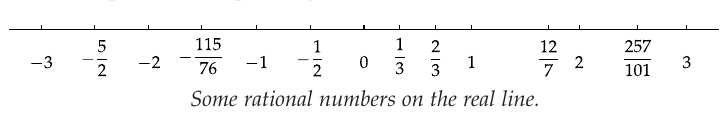
\includegraphics[scale=0.35]{real-line.png}
\end{figure}
\begin{itemize}
    \item if \( n\) is a positive integer then \( \frac{1}{n}\) is to the right of 0 by the length obtained by dividing the segment from \( 1 to 0\) in to \( n \) segments of equal length
\end{itemize}

\section{Is every Real Number a Rational}
\begin{figure}[h]
    \centering
    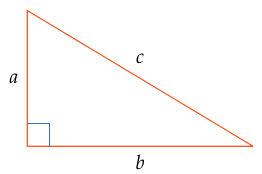
\includegraphics[scale=0.35]{irrational-geometry.png}
\end{figure}
\begin{itemize}
    \item \( c^{2} = a^{2} + b^{2} \). If \( a = 1, b = 1\) then \(c^{2} = 2 \). Then what rational number is \( c \)
    \item By trial and error, \( c = \left( \frac{99}{70} \right)^{2}  = \frac{9801}{4900}\) where the numerator just misses twice the denominator by 1. But this is not 2 but close to 2. Another number is \( \left( \frac{9369319}{6625109} \right)^{2} = 1.999999999999977\) , but not 2
    \item Greeks proved that it is impossible to find any rational number whose square is 2
\end{itemize}

\section{Proof: No rational number has a square equal to 2}
Let m and n are two integers
\[
    \left( \frac{m}{n} \right)^{2} = 2  
\]
By canceling any common factors, m and n are reduces to its lowest terms 

\[
    m^{2} = 2n^{2}
\]

this makes \(m^{2}\) even, hence \(m\) is an even. (The square of even is even and odd is odd). So \(m = 2k\) for some integer \(k\)

Substituting \(m = 2k\) in the equation gives, \(4k^{2} = 2n^{2} \), which results in 
\[
    2k^{2} = n^{2}
\]
which means \( n^{2}\) is even and therefore \(n \) is even
\\
\(\frac{m}{n} \) has common factors which contradicts the earlier assumption

\section{Irrational Number}

\begin{tcolorbox}[colback=yellow!5,
colframe=orange!80!black,
title=Irrational Number]
A real number that is not rational is \textbf{irrational number}
\end{tcolorbox}
\begin{itemize}
    \item \( \sqrt{2}\)
    \item \(3+\sqrt{2}\)
    \item \(8\sqrt{2}\)
\end{itemize}
% \chapter{Algebra of Real Numbers}
\author{Nithin}

\section{Properties of Real Numbers}
\begin{itemize}
    \item \textbf{Commutative Properties}
    \begin{itemize}
        \item Addition: $a + b = b + a$
        \item Multiplication: $a \cdot b = b \cdot a$
    \end{itemize}
    \vspace{5pt}

    \item \textbf{Associative Properties}
    \begin{itemize}
        \item Addition: $(a + b) + c = a + (b + c)$
        \item Multiplication: $(a \cdot b) \cdot c = a \cdot (b \cdot c)$
    \end{itemize}
    \vspace{5pt}
    \item \textbf{Distributive Property}
    \begin{itemize}
        \item $a \cdot (b + c) = (a \cdot b) + (a \cdot c)$
    \end{itemize}
    \vspace{5pt}
    \item \textbf{Identity Elements}
    \begin{itemize}
        \item Additive Identity: $a + 0 = a$
        \item Multiplicative Identity: $a \cdot 1 = a$
    \end{itemize}
    \vspace{5pt}
    \item \textbf{Inverse Elements}
    \begin{itemize}
        \item Additive Inverse: $a + (-a) = 0$
        \item Multiplicative Inverse (if $a \neq 0$): $a \cdot \frac{1}{a} = 1$
    \end{itemize}
\end{itemize}

\begin{itemize}
    \vspace{5pt}
    \item \textbf{Closure Property}
    \begin{itemize}
        \item Real numbers are closed under addition, subtraction, multiplication, and division (except division by zero).
    \end{itemize}
\end{itemize}

\section{Inequalities,Intervals and Absolute Value}
\subsection{Inequalities}
\subsubsection{Transitivity}
\begin{itemize}
    \item If $a < b$ and $b < c$, then $a < c$
    \end{itemize}
\subsubsection{Multiplication}
Suppose $a < b$
\begin{itemize}
    \item If $c > 0$, then $ac < bc$
    \item If $c <  0$, then $ ac > bc$
\end{itemize}

\subsection{Exercise}
Find all number \( x \) such that 
\[\frac{x-8}{x-4} < 3 \]
Our first step  is to multiply by \(x-4\)
Here there are two conditions:
\begin{enumerate}
    \item \( x-4 > 0 \)
    \[ x -8 < 3(x-4)  \implies x-8 < 3x-12 \implies 2x > 4  \implies x > 2\]
    But our initial assumption is \(x-4 > 0 \implies x > 4 \). As \( 4 > 2 \), original inequality holds if \( x > 4\)
    \item \( x-4 < 0 \)
    \[ x-8 > 3(x-4) \implies  x < 2 \]
    Initial assumption is \( x<4 \). As \( 2 < 4\), inequality holds for \( x < 2 \)
\end{enumerate}
The original inequality holds true for \( [x < 2 ,  x > 4 ] \)
or 
\[  (-\infty, 2) \cup (4,\infty) \]

\subsection{Inequalities}
\subsubsection{Additive Inverse}
If \( a < b \) then \( -a > -b \)
Direction of inequalities has to be reversed when taking additive inverses on both sides 
\subsubsection{Multiplicative Inverse}
If \( a < b \)
\begin{itemize}
    \item If \(a > 0, b > 0\), then \(\frac{1}{a} > \frac{1}{b} \)
    \item If \(a < 0 < b\), then \(\frac{1}{a} < \frac{1}{b} \)
\end{itemize} 

\subsection{What is a Set?}
A \textbf{set} is a well-defined collection of distinct objects, called \textbf{elements} or \textbf{members} of the set.
\textbf{Representation of a Set:}
\begin{itemize}
    \item \textbf{Roster Form:} List elements inside curly braces:
    \[
    A = \{1, 2, 3, 4\}
    \]
    \item \textbf{Set-Builder Notation:} Describe properties of elements:
    \[
    A = \{x \mid x \text{ is a positive integer less than 5}\}
    \]
\end{itemize}
\subsubsection{Membership}
\begin{itemize}
    \item If \(x\) belongs to \(A\), write \(x \in A\).
    \item If \(x\) does not belong to \(A\), write \(x \notin A\).
\end{itemize}

\subsection{Types of Sets}
\begin{itemize}
    \item \textbf{Finite Set:} A set with a countable number of elements. \\
    Example: \(A = \{1, 2, 3, 4\} \)
    
    \item \textbf{Infinite Set:} A set with an uncountable or infinite number of elements. \\
    Example: \(\mathbb{N} = \{1, 2, 3, \dots\} \)

    \item \textbf{Null Set:} A set with no elements, denoted as \(\emptyset\) or \(\{\}\).

    \item \textbf{Subset:} \(A \subseteq B\) if every element of \(A\) is in \(B\).

    \item \textbf{Universal Set:} A set containing all objects under consideration, usually denoted by \(U\).

    \item \textbf{Power Set:} The set of all subsets of \(A\), denoted as \(P(A)\). \\
    Example: If \(A = \{1, 2\}\), then \(P(A) = \{\emptyset, \{1\}, \{2\}, \{1, 2\}\} \)
\end{itemize}

\subsection{Set Operations}
\subsubsection{Union (\(\cup\))}
Combines elements of two sets:
\[
    A \cup B = \{x \mid x \in A \text{ or } x \in B\}
\]
\subsubsection{Intersection (\(\cap\))}
Elements common to both sets:
\[
    A \cap B = \{x \mid x \in A \text{ and } x \in B\}
\]
\subsubsection{Difference (\(A - B\))}
Elements in \(A\) but not in \(B\):
\[
    A - B = \{x \mid x \in A \text{ and } x \notin B\}
\]
\subsubsection{Complement (\(A^c\))}
Elements not in the set \(A\):
\[
    A^c = \{x \mid x \notin A\}
\]
\subsubsection{Examples}
\begin{itemize}
    \item The set of natural numbers: \(\mathbb{N} = \{1, 2, 3, \dots\} \)
    \item The set of integers: \(\mathbb{Z} = \{\dots, -3, -2, -1, 0, 1, 2, 3, \dots\} \)
    \item The set of even numbers: \(\{2, 4, 6, \dots\} \)
\end{itemize}

\subsection{What is an Interval?}
An \textbf{interval} is a set of real numbers that includes all the numbers between two given endpoints.
Intervals describe ranges of values on the real number line and are widely used in mathematics.

\subsection{Types of Intervals}
\begin{itemize}
    \item \textbf{Closed Interval (\([a, b]\))}: Includes both endpoints \(a\) and \(b\).
    \[
    [a, b] = \{x \in \mathbb{R} \mid a \leq x \leq b\}
    \]
    Example: \([2, 5] = \{x \mid 2 \leq x \leq 5\} \).
    \vspace{5pt}

    \item \textbf{Open Interval (\((a, b)\))}: Excludes both endpoints \(a\) and \(b\).
    \[
    (a, b) = \{x \in \mathbb{R} \mid a < x < b\}
    \]
    Example: \((2, 5) = \{x \mid 2 < x < 5\} \).
\end{itemize}

\subsection{Half-Open or Half-Closed Intervals}
\begin{itemize}
    \item \textbf{Left-Closed, Right-Open (\([a, b)\))}:
    \[
    [a, b) = \{x \in \mathbb{R} \mid a \leq x < b\}
    \]
    Example: \([2, 5) = \{x \mid 2 \leq x < 5\} \).
    \vspace{5pt}

    \item \textbf{Left-Open, Right-Closed (\((a, b]\))}:
    \[
    (a, b] = \{x \in \mathbb{R} \mid a < x \leq b\}
    \]
    Example: \((2, 5] = \{x \mid 2 < x \leq 5\} \).
\end{itemize}

\subsection{Infinite Intervals}
\begin{itemize}
    \item \((a, \infty)\): All numbers greater than \(a\).
    \[
    (a, \infty) = \{x \in \mathbb{R} \mid x > a\}
    \]
    Example: \((3, \infty)\) includes all numbers greater than 3.

    \item \((-\infty, b)\): All numbers less than \(b\).
    \[
    (-\infty, b) = \{x \in \mathbb{R} \mid x < b\}
    \]
    Example: \((-\infty, 4)\) includes all numbers less than 4.

    \item \((-\infty, \infty)\): The entire real number line.
    \[
    (-\infty, \infty) = \mathbb{R}
    \]
\end{itemize}

\subsection{Summary of Interval Types}
\begin{tabular}{|c|c|c|}
    \hline
    \textbf{Type} & \textbf{Interval Notation} & \textbf{Description} \\
    \hline
    Closed         & \([a, b]\)      & Includes both endpoints \(a, b\) \\
    Open           & \((a, b)\)      & Excludes both endpoints \(a, b\) \\
    Half-Open Left & \([a, b)\)      & Includes \(a\), excludes \(b\) \\
    Half-Open Right & \((a, b]\)     & Excludes \(a\), includes \(b\) \\
    Infinite Left  & \((-\infty, b)\)& All \(x < b\) \\
    Infinite Right & \((a, \infty)\) & All \(x > a\) \\
    Entire Line    & \((-\infty, \infty)\) & All real numbers \\
    \hline
\end{tabular}

\subsection{What is Absolute Value?}
The \textbf{absolute value} of a number is its distance from zero on the number line, regardless of direction. It is always non-negative.
For a real number \(x\), the absolute value, denoted as \(|x|\), is defined as:
\[
|x| =
\begin{cases} 
x, & \text{if } x \geq 0, \\
-x, & \text{if } x < 0.
\end{cases}
\]
Breaking the absolute value: 
\begin{itemize}
    \item \( |f(x)| \leq c \quad \implies \quad -c \leq f(x) \leq c \)
    \item \( |f(x)| \geq c \quad \implies \quad f(x) \leq -c \quad \text{or} \quad f(x) \geq c \)
\end{itemize}

\subsection{Examples of Absolute Value}
\begin{itemize}
    \item \(|3| = 3\) \quad (because \(3 \geq 0\))
    \item \(|-5| = -(-5) = 5\) \quad (because \(-5 < 0\))
    \item \(|0| = 0\) \quad ( because \(0\) is neither positive nor negative)
\end{itemize}

\subsection{Properties of Absolute Value}
\begin{itemize}
    \item \textbf{Non-Negativity:} \(|x| \geq 0\) for all \(x\).
    \item \textbf{Identity Property:} \(|x| = 0 \quad \text{if and only if } x = 0\)
    \item \textbf{Multiplicative Property:} \(|x \cdot y| = |x| \cdot |y|\).
    \item \textbf{Triangle Inequality:} \( |x + y| \leq |x| + |y| \).
    \item \textbf{Distance Interpretation:} \(|x - y|\) represents the distance between \(x\) and \(y\).
\end{itemize}

\subsection{Exercises}
\subsubsection{Ball Bearings}
Ball bearings need to have extremely accurate sizes to work correctly. The ideal diameter of a particular ball bearing is 0.8 cm, but a ball bearing is declared acceptable if the error in the diameter size is less than 0.001 cm. Write the inequality for acceptance criteria
\subsubsection{Solution}
The ball bearings are acceptable if the diameter \(d\) satisfies:
\[
|d - 0.8| < 0.001
\]

\subsection{Exercises}
Find all numbers \(t \) such that \( |3t-4| = 10\)
Solution :
\[ 3t -4  = 10  \; or \; 3t-4 = -10  \implies t = \frac{14}{3}, t = -2 \]

\subsection{Exercise}
Find all numbers \(x\) such that \( \left| \frac{3x-5}{x-1} \right|< 2 \)
Solution :
\[ |3x-5| < 2 |x-1| \]
\begin{enumerate}
    \item \(x-1 > 0 \)
\end{enumerate}
Breaking the absolute value:
\begin{flalign}
    &\implies -2(x-1) < 3x-5 < 2(x-1) = -2x + 7 < 3x < 2x + 3  \ 
    &\implies 3x > -2x+7   \; \& \; 3x < 2x + 3  
\end{flalign}

\subsection{Exercise}
Solving for \( 3x < 2x + 3\)
\begin{flalign}
    &\implies x < 3 \\
\end{flalign}
Solving for \(3x > -2x+7 \)
\begin{flalign}
    &\implies 3x > -2x+7 \implies 5x > 7 \implies x > 7/5 \\
    &\implies x \in (7/5,3) 
\end{flalign}

\subsection{Exercise} 
\begin{enumerate}
    \setcounter{enumi}{1}
    \item \(x-1 < 0 \implies x < 1 \)
\end{enumerate}
\begin{flalign}
    &\implies |3x-5| < 2 |x-1| == |3x-5| < -2(x-1) \\
    &\implies         3x-5 < -2(x-1) \; \text{ and } \; -(3x-5) < -2(x-1) \\
    &\implies  3x-5 < -2(x-1)  \; \text{ and } \; 3x-5 > 2(x-1) 
\end{flalign}
\begin{flalign}
    &3x-5 < -2(x-1) \implies  3x < -2x+7 \implies 5x < 7 \implies x < 7/5 \\
    &\implies 3x-5 > 2(x-1) \implies 3x > 2x + 3 \implies x > 3 
\end{flalign}
Here \( x > 3\) is inconsistent with our assumption \(x < 1\). So for \(x<1\) there are no values of \(x\) satisfying the inequality
% \chapter{Introduction to Functions}
\author{Nithin}

\section{Domain,Range and Equality}

\subsection{What is a Function ?}
A function associates every number in some set of real numbers, called the domain of the function, with exactly one real number.

\subsection{Domain}
If a function is defined by a formula, with no domain specified, then the domain is assumed to be the set of all real numbers for which the formula makes sense and produces a real number.

\subsubsection{Example 3}
Find the domain of the function \(f\)  defined by \[f (x) = (3x-1)^2 \]

\subsubsection{Example 4}
Find the domain of the function \(f\) defined by \[h (t) = \frac{t^2 + 3t + 7}{t-4} \]

\subsubsection{Example 6}
Find the domain of the function g defined by \[g(x) = \sqrt{|x|-5}\]

\subsection{Range}
The range of a function \(f\) is the set of all numbers \(y\) such that \(f (x) = y\) for at least one \(x\) in the domain of \(f\).

\subsubsection{Example 4}
The domain of \(f\) is the interval \( [2, 5] \), with \(f\) defined on this interval by the equation \(f (x) = 3x + 1\).
Solution:
\[ y = f(x) = 3x+1 \]
\[ 2 \leq \frac{y-1}{3} \leq 5. \]
\[ 7 \leq y \leq 16. \]

\subsubsection{Example 5}
The domain of \(g\) is the interval \([1,20]\), with \(g\) defined on this interval by the equation
\[ g(x) = |x - 5|. \]
Is \(2\) in the range of \(g\)?
Solution:
\[ y =  |x-5| \]
for \(x-5>0 \),\(y = x-5 \implies x = y+5 \)
\[ 5 < y+5 \leq 20  \implies  0 < y \leq 15 \]
for \(x-5<0 \), \(y = -(x-5) \implies y = -x+5 \implies 5-y = x \)
\[ 1 \leq 5-y \leq 5  \implies -4 \leq -y \leq 0 \implies  4 \geq y \geq 0 \]

\subsection{Equality of Functions}
Two functions are equal if and only if they have the same domain and the same value at every number in that domain.

\subsubsection{Example}
Suppose \(f\) is the function whose domain is the set of real numbers, with \(f\) defined on this domain by
\[f (x) = x^2\]
Suppose \(g\) is the function whose domain is the set of positive numbers, with \(g\) defined on this domain by
\[g(x) = x^2\]
Are \(f\) and \(g\) equal functions?

\subsubsection{Example 2}
Suppose \(f\) and \(g\) are functions whose domain is the set consisting of the two numbers \(\{1, 2\}\) with \(f\) and \(g\) defined on this domain by the formulas
\[f (x) = x^2\] and \(g(x) = 3x-2\).
Are \(f\) and \(g\) equal functions?

\section{Analytical Geometry}
\subsection{What is Analytic Geometry?}
\begin{itemize}
    \item \textbf{Analytic Geometry} (also called \textit{coordinate geometry} or \textit{Cartesian geometry}) bridges algebra and geometry.
    \item It uses a coordinate system to study geometric shapes and properties.
    \item Geometric objects are represented as algebraic equations.
\end{itemize}

\subsection{Co-ordinate Plane}
\begin{figure}[h]
    \centering
    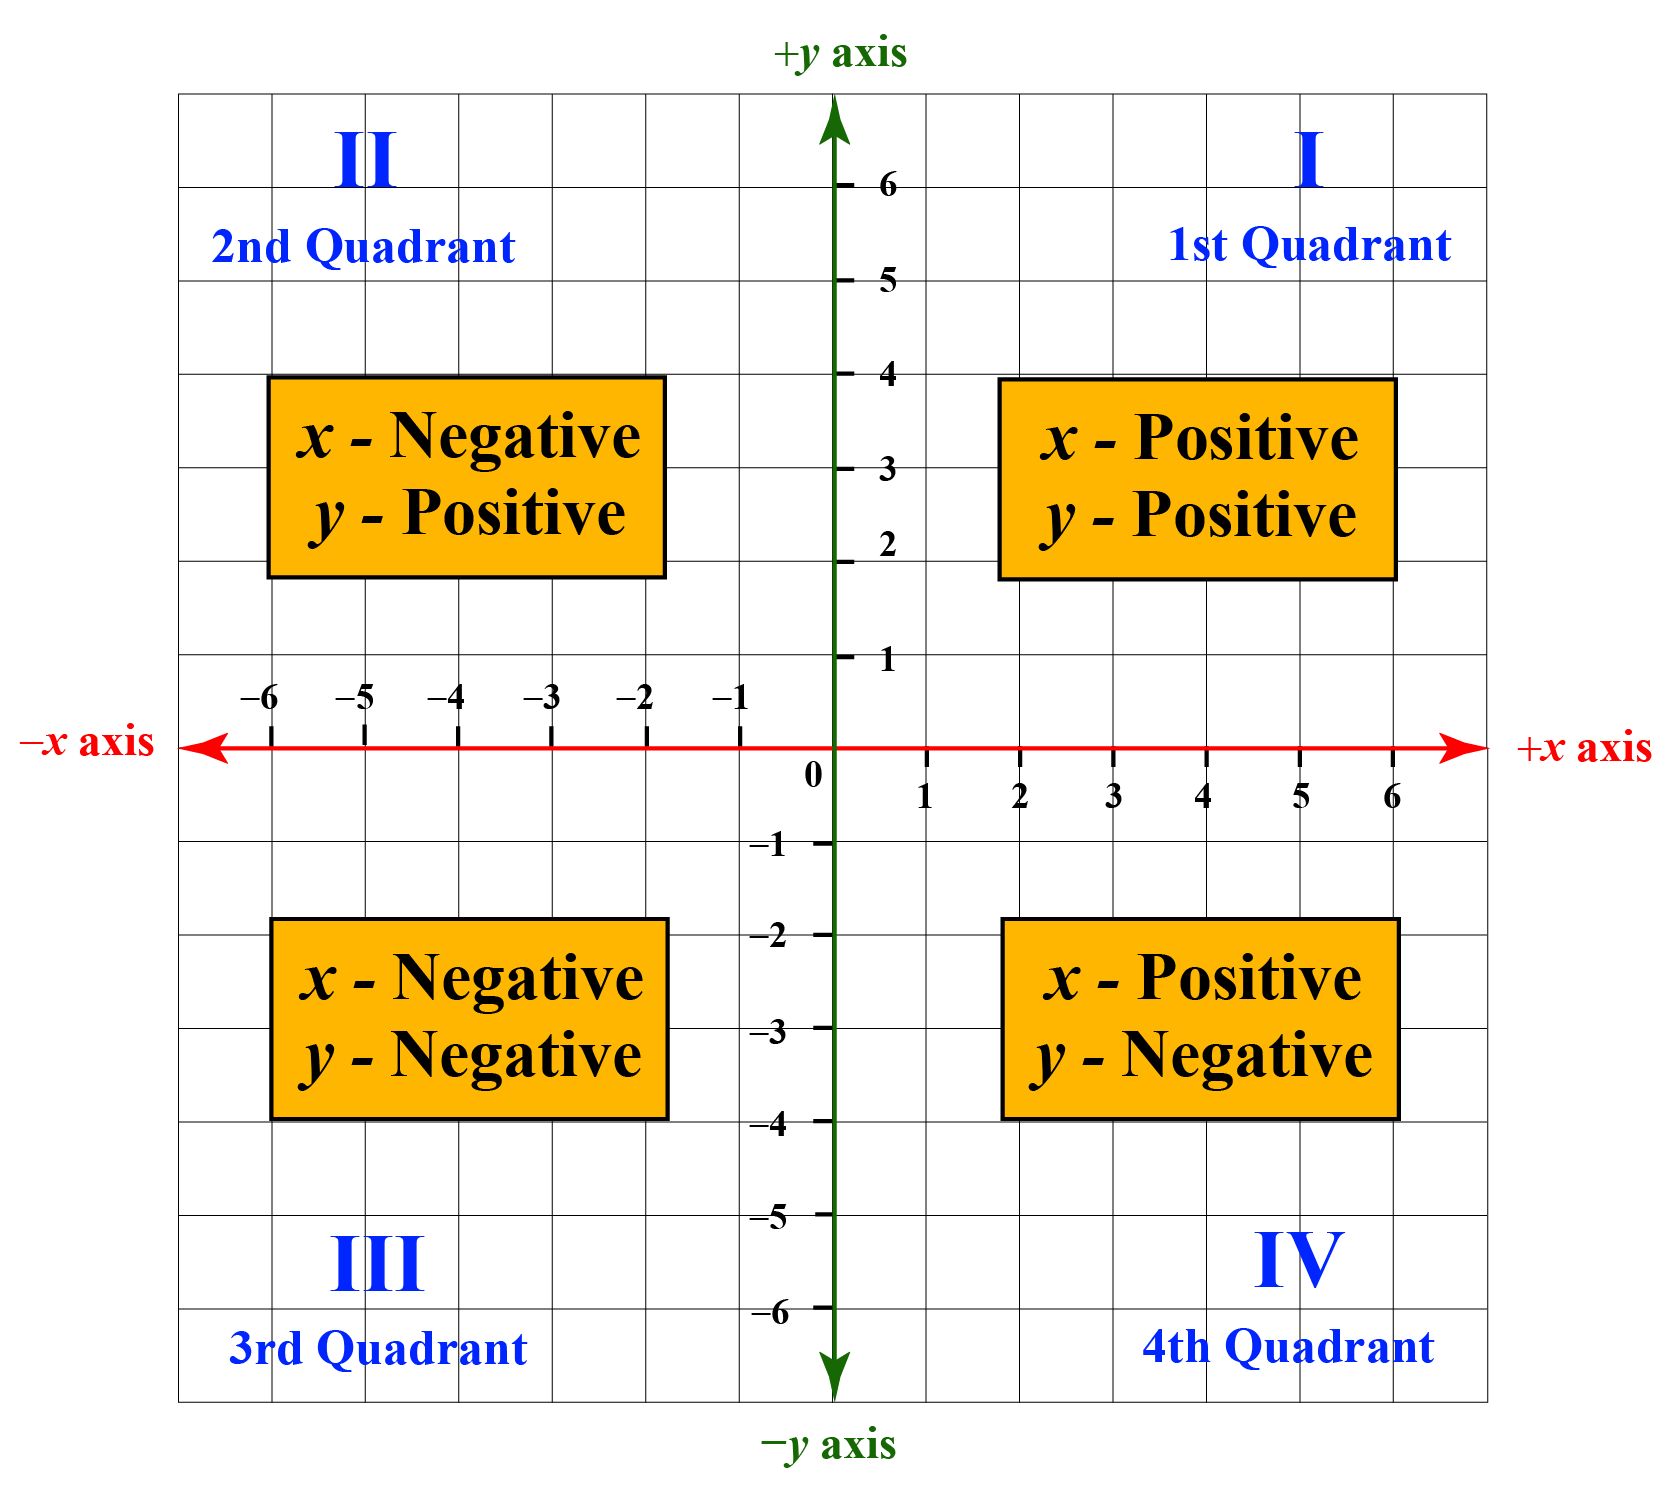
\includegraphics[scale=0.23]{cartesian.png}
\end{figure}
The plane with this system of labeling is often called the \textbf{Cartesian plane} in honor of the French mathematician Rene Descartes(1596-1650), who described this technique in his 1637 book Discourse on Method.

\subsection{Graph Functions}
The graph of a function \(f\) is the set of points of the form \(x, f (x)\) as x varies over the domain of \(f\).

\subsubsection{Graphs}
\begin{figure}[h]
  \centering
  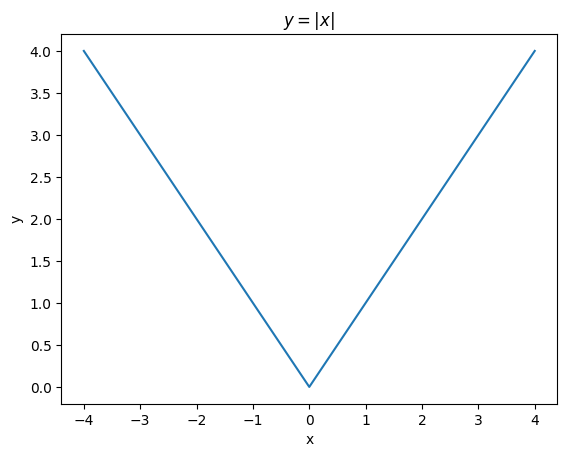
\includegraphics[scale=0.3]{graph.png}
\end{figure}
\begin{figure}[h]
  \centering
  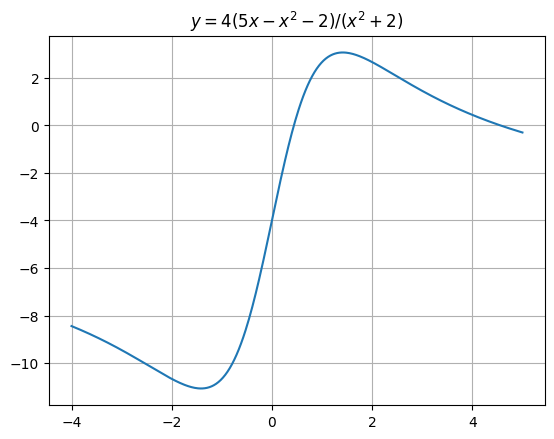
\includegraphics[scale=0.3]{graph2.png}
\end{figure}

\subsection{Checking for a function: Vertical line test}
The line \(x=1\) intersects the curve at two points. That is that for each \(x\) value there are multiple \(y\) values which is contradicting to definition of a function.
\subsubsection{Vertical Line Test}
A set of points in the coordinate plane is the graph of some function if and only if every vertical line intersects the set in at most one point.

\section{Average Rate of change}
The rate of change describes how an output quantity changes relative to the change in the input quantity. The unit on a rate of change.
The \textbf{average rate of change} of a function \(f\) over an interval \([x_{1}, x_{2}]\) is given by
\[ =\frac{\Delta y}{\Delta x} =\frac{f(x_{2}) - f(x_{1})}{x_{2} - x_{1}} \]

\subsection{Increasing, Decreasing and Constant Functions}
\begin{figure}
  \centering
  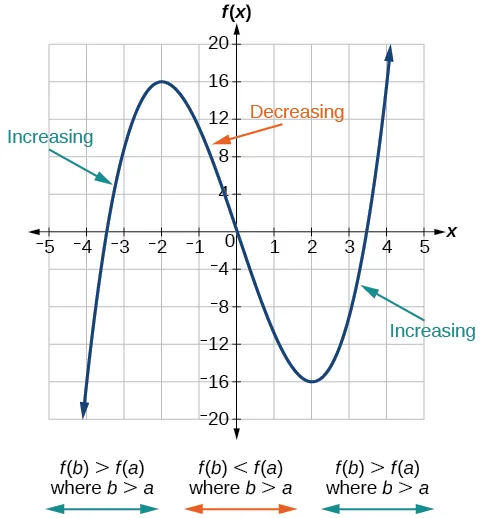
\includegraphics[scale=0.3]{inc-dec.png}
\end{figure}

\subsubsection{Increasing Function}
A function \(f\) is said to be increasing on an interval \((a, b)\) if for any \(x_{1}, x_{2}\) in \((a, b)\) with \(x_{1} < x_{2}\), we have \(f(x_{1}) < f(x_{2})\) or it has a positive rate of change over the interval.

\subsubsection{Decreasing Function}
A function \(f\) is said to be decreasing on an interval \((a, b)\) if for any \(x_{1}, x_{2}\) in \((a, b)\) with \(x_{1} < x_{2}\), we have \(f(x_{1}) > f(x_{2})\) or it has a negative rate of change over the interval.

\subsubsection{Constant Function}
A function \(f\) is said to be constant on an interval \((a, b)\) if for any \(x_{1}, x_{2}\) in \((a, b)\) with \(x_{1} < x_{2}\), we have \(f(x_{1}) = f(x_{2})\) or it has a zero rate of change over the interval.

\subsection{Local Maxima and Local Minima}
\begin{figure}
  \centering
  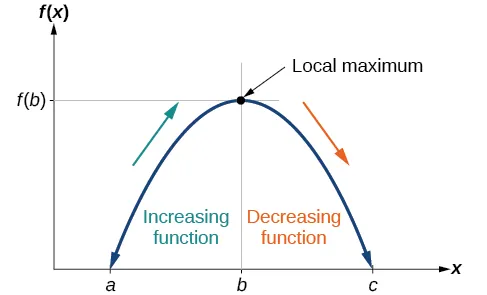
\includegraphics[scale=0.5]{max-min.png}
\end{figure}

\subsubsection{Local Maximum}
A function \(f\) has a \textbf{local maximum} at \(x = c\) if there exists an interval \((a, b)\) containing \(c\) such that
\[ f(c) \geq f(x) \quad \text{for all } x \in (a, b) \]

\subsubsection{Local Minimum}
A function \(f\) has a \textbf{local minimum} at \(x = c\) if there exists an interval \((a, b)\) containing \(c\) such that
\[ f(c) \leq f(x) \quad \text{for all } x \in (a, b) \]

\section{Function Transformation}
\subsection{Vertical Transformations}
\subsubsection{Shifting a graph up or down}
Suppose \(f \) is a function and \(a > 0\). Upshift \(g\) and  Downshift \(h\) by
\[g(x) = f (x) + a \;\; h(x) = f (x) - a \]
\begin{figure}[h]
  \centering
  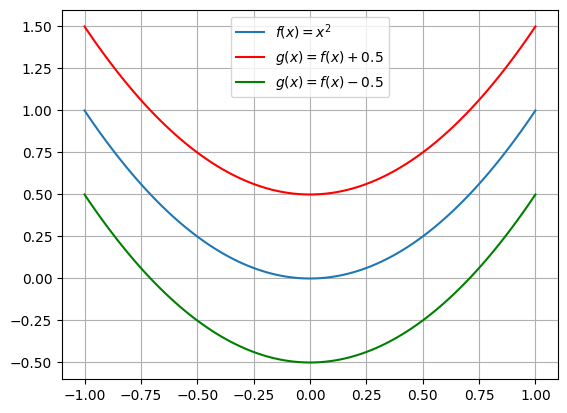
\includegraphics[scale=0.4]{vertical_shift.png}
\end{figure}

\subsubsection{Vertical Stretch}
Suppose \(f\) is a function and \(c > 0\). Define a function \(g\) by
\[g(x) = c f (x)\]
\begin{figure}[h]
  \centering
  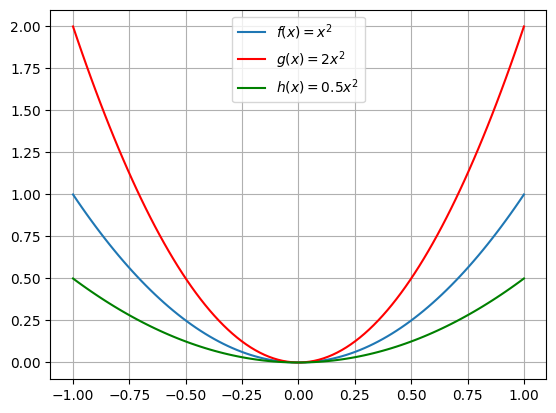
\includegraphics[scale=0.5]{vertical_stretch.png}
\end{figure}

\subsubsection{Flipping along the Vertical Axis}
Vertical fliiping of \(f(x) \) is
\[g(x) = - f (x) \]
\begin{figure}[h]
  \centering
  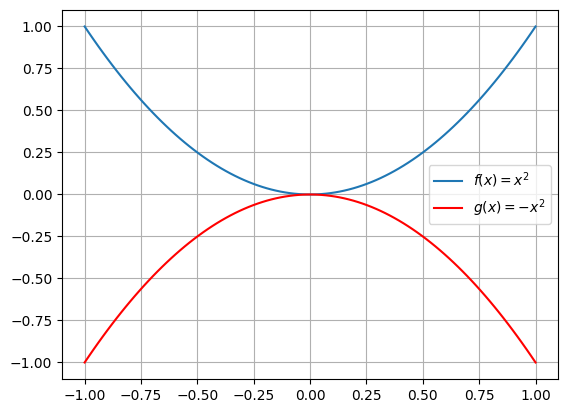
\includegraphics[scale=0.5]{vertical_flip.png}
\end{figure}

\subsection{Horizontal Transformation}
\subsubsection{Horizontal Shift}
\[g(x) = f(x+a), h(x) = f(x-a)\]
\begin{figure}[h]
  \centering
  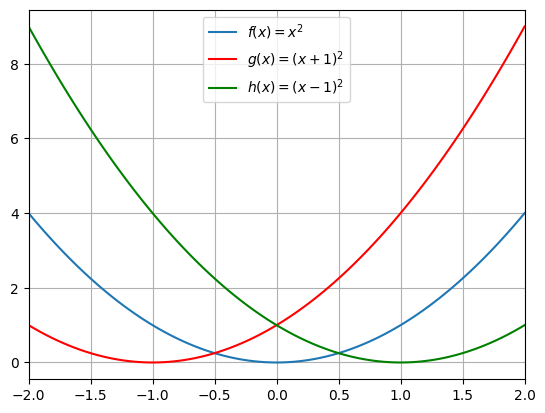
\includegraphics[scale=0.5]{horizontal-shift.png}
\end{figure}

\subsubsection{Horizontal Stretching}
\[g(x) = f(cx)\]
\begin{figure}[h]
  \centering
  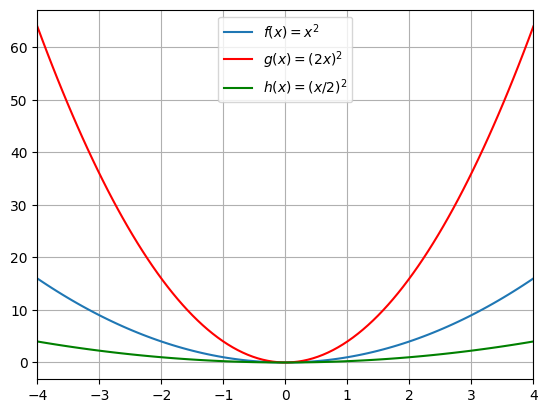
\includegraphics[scale=0.55]{horizontal-stretch.png}
\end{figure}

\subsection{Flipping ac the Vertical Axis}
\subsubsection{Horizontal Stretching}
\[g(x) = f(-x)\]
\begin{figure}[h]
  \centering
  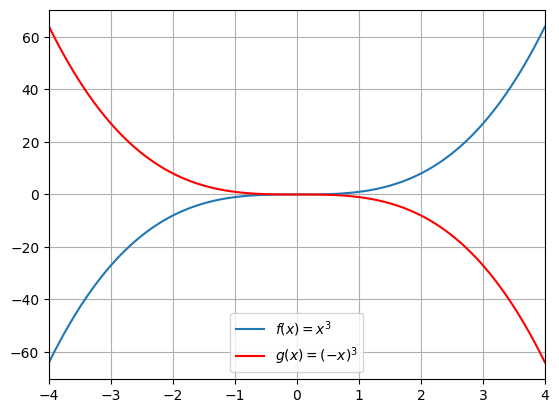
\includegraphics[scale=0.55]{vertical-axis-flip.png}
\end{figure}

\subsection{Combinations of vertical Transformation}
\begin{figure}[h]
  \centering
  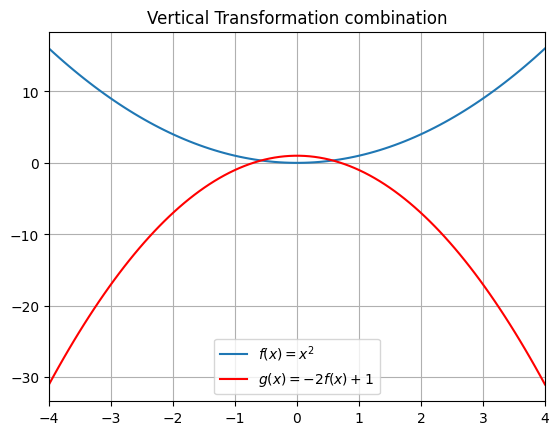
\includegraphics[scale=0.55]{vertical_combination.png}
\end{figure}

\subsection{Even Functions}
\[ f(-x) = f(x) \quad \text{for all } x \text{ in the domain} \]
Example: \( f(x) = x^2, \quad f(x) = \cos x \)
The graph of an even function is symmetric across the vertical axis.
\begin{figure}
\centering
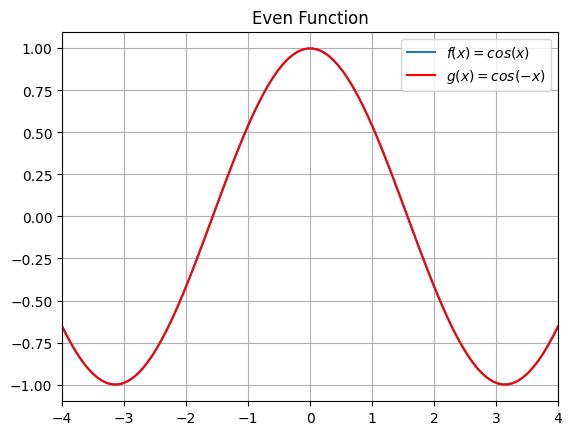
\includegraphics[width=0.45\linewidth]{even.png}
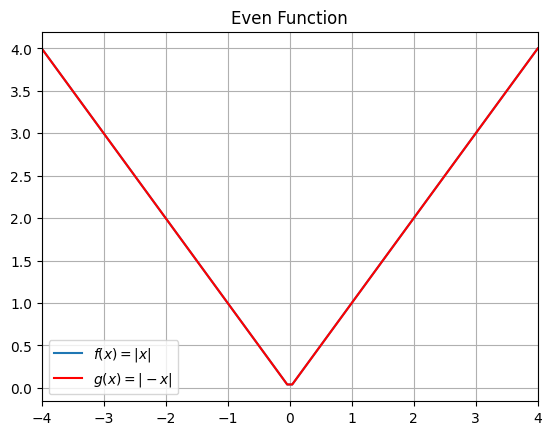
\includegraphics[width=0.45\linewidth]{even2.png}
\end{figure}

\subsection{Odd Function}
\[ f(-x) = -f(x) \quad \text{for all } x \text{ in the domain} \]
Example: \( f(x) = x^3, \quad f(x) = \sin x \)
The graph of an even function is symmetric if flipped or rotated 18 across the origin.
\begin{figure}
\centering
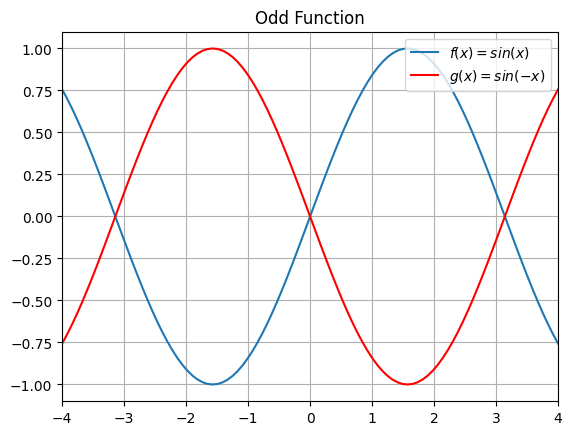
\includegraphics[width=0.45\linewidth]{odd.png}
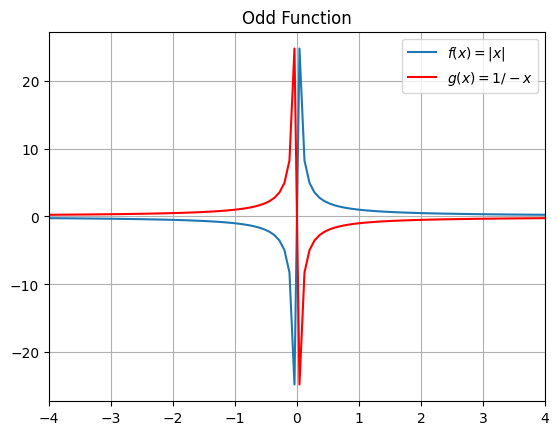
\includegraphics[width=0.45\linewidth]{odd2.png}
\end{figure}

\section{Function Composition}
\subsection{Algebra of Functions}
Suppose \(f\) and \(g\) are functions. We can define new functions from \(f\) and \(g\) as follows: \\
\textbf{Sum:}
\[ (f+g)(x) = f(x) + g(x) \]
\textbf{Difference:}
\[ (f-g)(x) = f(x) - g(x) \]
\textbf{Product:}
\[ (f\cdot g)(x) = f(x) \cdot g(x) \]
\textbf{Quotient:}
\[ \left(\frac{f}{g}\right)(x) = \frac{f(x)}{g(x)} \quad \text{provided } g(x) \neq 0. \]
\textbf{Note:} If \(f\) and \(g\) have domains \(D_f\) and \(D_g\), then these operations are defined on the intersection \(D_f \cap D_g\). In the case of the quotient, it is defined on
\[ \{x \in D_f \cap D_g : g(x) \neq 0\}. \]

\subsection{Exercise}
\( f(x)  = \sqrt{x-3}\) and \(g(x) = \sqrt{8 - x } \)
Evaluate
\begin{enumerate}
  \item[a.] \((f+g)(x)\)
  \item[b.]  \((fg)(x)\)
  \item[c.] Find the domain of above
\end{enumerate}
Sol:
\begin{enumerate}
  \item[a.] \(\sqrt{x-3} + \sqrt{8-x} \)
  \item[b.] \(\sqrt{(x-3)(8-x)} \)
  \item[c.]  Domian of \begin{enumerate}
    \item[a.] \(x\geq 3 \)
    \item[b.] \(x \leq 8 \)
    \item[c.] \( 3 \leq x \leq 8 \)
  \end{enumerate}
\end{enumerate}

\subsection{Function Composition}
\subsubsection{Definition:}
If \( f(x) \) and \( g(x) \) are functions, then the composition of \( f \) and \( g \), denoted by \( f \circ g \), is defined by
\[ (f \circ g)(x) = f(g(x)). \]
\textbf{Example:}
Consider the function
\[ h(x) = \sqrt{x+3}. \]
We can express \( h(x) \) as a composition of two functions \( f \) and \( g \) where:
\[ f(x) = \sqrt{x} \quad \text{and} \quad g(x) = x+3. \]
Then,
\[ h(x) = f(g(x)) = f(x+3) = \sqrt{x+3}. \]

\subsection{Exercise}
\( f(x) = \frac{1}{x-4} \) and \( g(x) = x^{2} \)
\begin{enumerate}
  \item \(f \circ g \)
  \item \( g \circ f \)
  \item domian of \(f \circ g \)
  \item domain of \( g \circ f \)
\end{enumerate}
Sol:
\begin{enumerate}
  \item  \(f(g(x)) = \frac{1}{x^{2} - 4}\)
  \item \(g(f(x)) = (\frac{1}{x-4})^{2}\)
  \item \(R - \{-2,2\} \)
  \item \(R - \{4\} \)
\end{enumerate}

\subsection{Composition Machine}
\begin{figure}
  \centering
  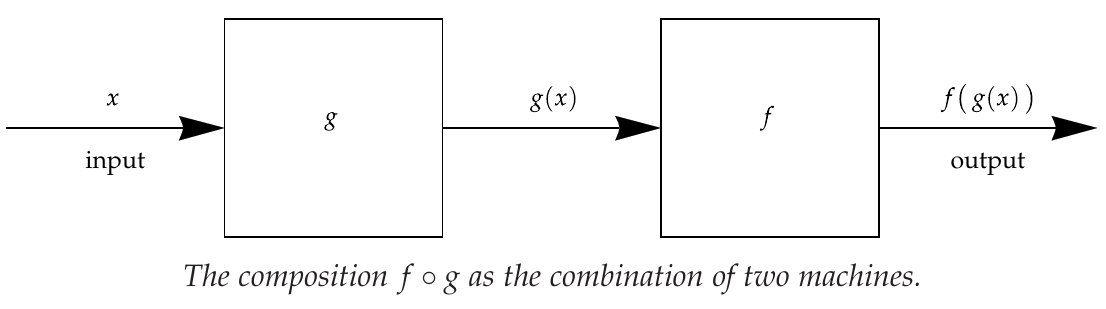
\includegraphics[scale=0.3]{composition.png}
\end{figure}

\subsection{Excersise}
\textbf{Problem:} Suppose your cell phone company charges \(\$0.05\) per minute plus \(\$0.47\) for each call to China.
\begin{enumerate}
  \item[(a)] Find a function \(p\) that gives the amount charged by your cell phone company for a call to China as a function of the number of minutes \(m\).
  \item[(b)] Suppose the tax on cell phone bills is 6\% plus \(\$0.01\) for each call. Find a function \(t\) that gives your total cost, including tax, for a call to China as a function of the amount charged by your cell phone company.
  \item[(c)] Explain why the composition \(t \circ p\) gives your total cost, including tax, of making a cell phone call to China as a function of the number of minutes.
  \item[(d)] Compute a formula for \(t \circ p\).
  \item[(e)] What is your total cost for a ten-minute call to China?
\end{enumerate}

\subsection{Solution}
\textbf{(a)} The company charges \(\$0.05\) per minute plus a fixed charge of \(\$0.47\) per call. Hence, the pre-tax charge function is
\[ p(m)=0.05m+0.47. \]
\textbf{(b)} The tax on the cell phone bill is 6\% of the pre-tax amount plus an additional \(\$0.01\) per call. Thus, if the pre-tax charge is \(x\), the total cost function (including tax) is
\[ t(x)=1.06x+0.01. \]
\textbf{(c)} The composition \(t \circ p\) means we first compute the pre-tax charge \(p(m)\) for a call of \(m\) minutes, and then we apply the tax function \(t\) to this amount. In other words, \(t(p(m))\) gives the total cost, including tax, as a function of the number of minutes.
\textbf{(d)} To compute the composition, substitute \(p(m)\) into \(t\):
\[ (t \circ p)(m)=t(p(m))=1.06\bigl(0.05m+0.47\bigr)+0.01. \]
Distribute \(1.06\):
\[ 1.06(0.05m)=0.053m \quad \text{and} \quad 1.06(0.47)=0.4982. \]
Thus,
\[ (t \circ p)(m)=0.053m+0.4982+0.01=0.053m+0.5082. \]
\textbf{(e)} For a ten-minute call (\(m=10\)):
\[ (t \circ p)(10)=0.053(10)+0.5082=0.53+0.5082=1.0382. \]
Rounded to the nearest cent, the total cost is approximately \(\$1.04\).

\subsection{Identity Function}
The identity function is defined by
\[ I(x) = x \quad \text{for every number } x. \]
The function \(I\) is the identity for composition. If \(f\) is any function, then
\[ f \circ I = I \circ f = f. \]

\subsection{Decomposing the Functions}
\subsubsection{Function Decomposition}
\[ T(y) = \frac{|y^{2} -3|}{|y^{2} - 7|} \]
Sol:
\[f(y) = |y|, g(y) = \frac{y^{2}-3}{y^{2}-7} \]
\[ f(y) = \frac{|y-3|}{|y-7|}, g(y) = y^{2}\]
Composition is associative if \(f,g, h\) are functions then
\[(f \circ g) \circ h  = f \circ (g \circ h) \]

\subsection{Example}
\subsubsection{Composition of three functions}
\[T(x) = \left| \frac{x^{2}-3}{x^{2} - 7}  \right| \]
Sol:
\[f(x) = |x|, g(x) = \frac{x-3}{x-7}, h(x) = x^{2}\]

\subsection{Linear Functions}
A linear function is a function \(h\) of the form
\[h(x) = mx + b\]
where \(m\) and \(b\) are numbers.

\subsection{Linear Functions as Composition}
\subsubsection{Vertical Transformations as Compositions}
A funtion \(g(x)\) is defined by
\[g(x)= -2f(x)+1\]
Write \(g(x)\) as a the composition of a linear function with \(f(x)\)
\[h(x) = -2x + 1 \]
\[\implies g(x) = h(f(x)) \implies g = h \circ f \]

\subsubsection{Horizontal Transformations as Compositions}
A funtion \(g(x)\) is defined by
\[g(x)= f(2x)+1\]
Write \(g(x)\) as a the composition of a linear function,  \(f(x)\) and other linear function
\[h(x) = x + 1, p(x) = 2x \]
\[\implies g(x) = h(f(p(x))) \implies g = h \circ f \circ p \]

\section{Inverse Functions}
\subsection{Inverse Function: Example}
Consider the function \( f: \mathbb{R} \to \mathbb{R} \) defined by
\[ y = \frac{9}{5}x + 32, \]
which converts a temperature \( x \) in Celsius to Fahrenheit \( y \). 
The inverse function \( f^{-1} \) converts Fahrenheit back to Celsius:
\[ f^{-1}(y) = \frac{5}{9}(y - 32). \]
Verifying that these functions are inverses:
\[ f^{-1}(f(x)) = \frac{5}{9}\Bigl(\frac{9}{5}x + 32 - 32\Bigr) = x, \]
\[ f(f^{-1}(f)) = \frac{9}{5}\Bigl(\frac{5}{9}(y - 32)\Bigr) + 32 = y. \]

\subsection{One-to-One Function}
A function \(f\) is called one-to-one if for each number \(y\) in the range of \(f\) there is
exactly one number \(x\) in the domain of \(f\) such that \(f (x) = y\).

\subsection{Inverse Function}
\subsubsection{Definition}
Suppose \( f \) is a one-to-one function.
\begin{itemize}
  \item If \( y \) is in the range of \( f \), then \( f^{-1}(y) \) is defined to be the number \( x \) such that \( f(x) = y \).
  \item The function \( f^{-1} \) is called the \emph{inverse function} of \( f \).
\end{itemize}
\textbf{Short version:}
\begin{itemize}
  \item \( f^{-1}(y) = x \) means \( f(x) = y \).
\end{itemize}

\begin{figure}
  \centering
  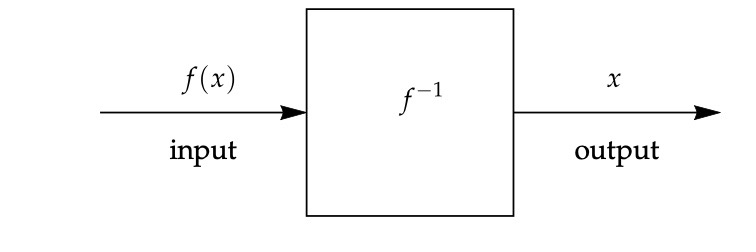
\includegraphics[scale=0.4]{inverse.jpeg}
\end{figure}

\subsection{Domain and Range of an Inverse Function}
If \( f \) is a one-to-one function, then:
\begin{itemize}
  \item The domain of \( f^{-1} \) equals the range of \( f \).
  \item The range of \( f^{-1} \) equals the domain of \( f \).
\end{itemize}

\subsection{Increasing and Decreasing Function}
\subsubsection{Increasing}
A function \(f\) is called increasing if \(f (a) < f (b)\) whenever \(a < b\) and \(a, b \) are in
the domain of \(f\).

\subsubsection{Decreasing}
A function \(f\) is called decreasing if \(f (a) >  f (b)\) whenever \(a < b\) and \(a, b \) are in
the domain of \(f\).

\subsubsection{Increasing and decreasing functions are one-to-one}
\begin{itemize}
  \item Every increasing function is one-to-one
  \item Every decreasing function is one-to-one.
\end{itemize}

\subsection{Exercise}
\begin{figure}
  \centering
  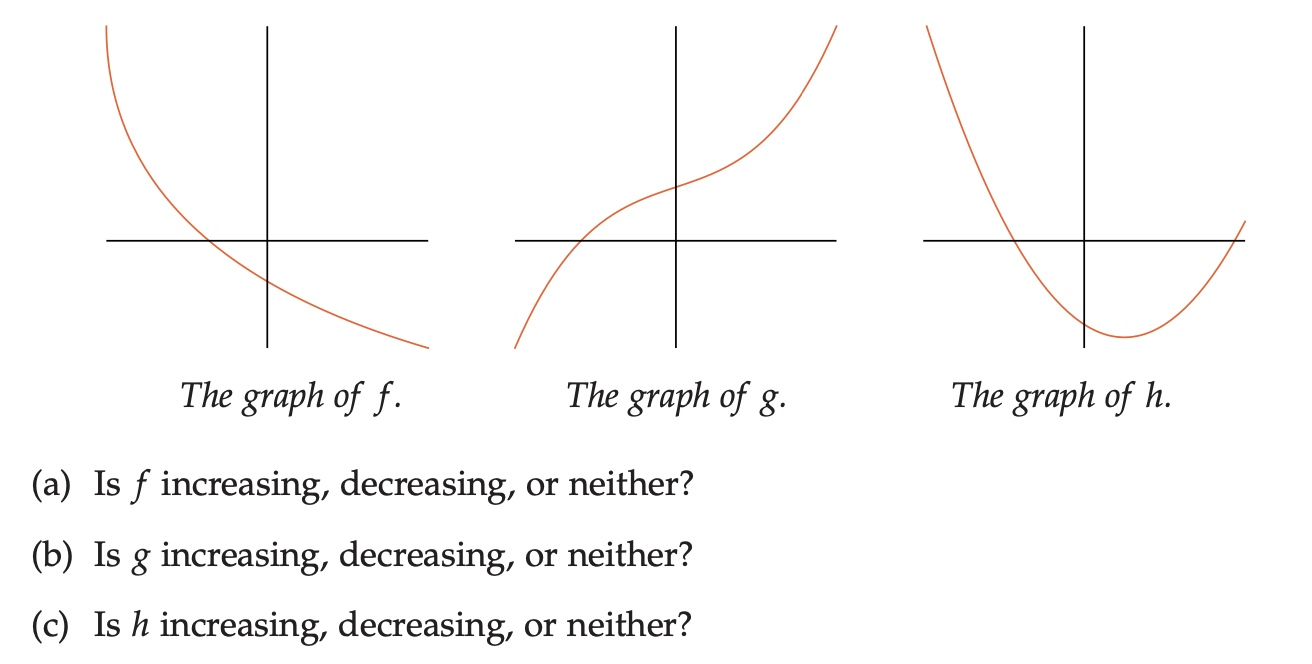
\includegraphics[scale=0.2]{increase.jpeg}
\end{figure}
\begin{enumerate}
  \item[a.] Decreasing
  \item[b.] Increasing
  \item[c.] Neither
\end{enumerate}

\subsection{Do all one-to-one maps are increasing or decreasing ?}
% \begin{figure}
%   \centering
%   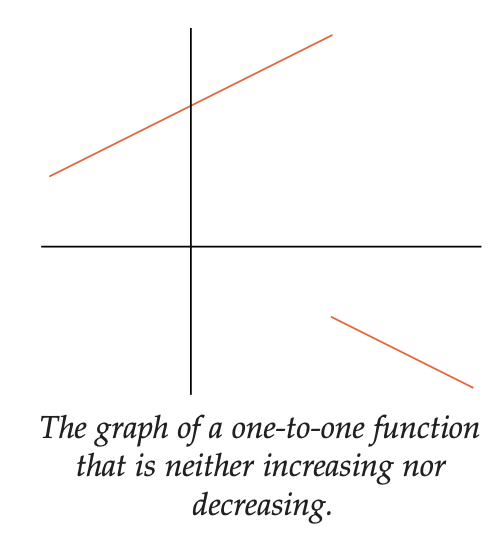
\includegraphics[scale=0.6]{non-increse-decrese.png}
% \end{figure}

\subsection{Increasing and Decreasing Functions}
\subsubsection{Inverses of increasing and decreasing functions}
\begin{itemize}
  \item The inverse of an increasing function is increasing.
  \item The inverse of a decreasing function is decreasing.
\end{itemize}

% \chapter{Linear,Quadratic, Polynomial and Rational Functions}
\author{Nithin}

\section{Lines and Linear Function}
\subsection{Slope}
\begin{figure}
  \centering
  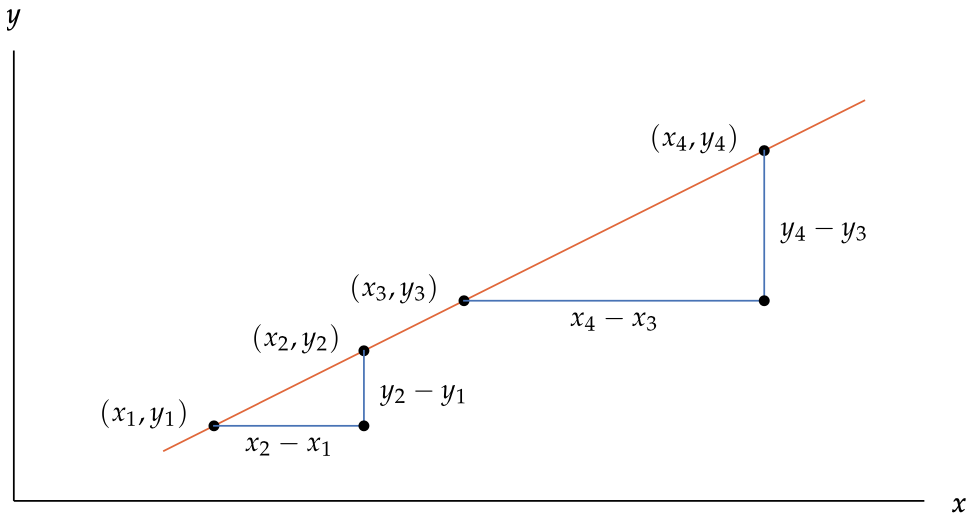
\includegraphics[scale=0.25]{slope.png}
\end{figure}
\[\frac{y_{2} - y_{1}}{x_{2} - x_{1}} = \frac{y_{4} - y_{3}}{x_{4} - x_{3}}\]

If \(x_{1},y_{1}\) and \(x_{2},y_{2}\) are any two points on a line with \(x_{1} \neq x_{2}\), then the \textbf{slope} of the line is
\[\frac{y_{2} - y_{1}}{x_{2} - x_{1}}\]

\begin{figure}
  \centering
  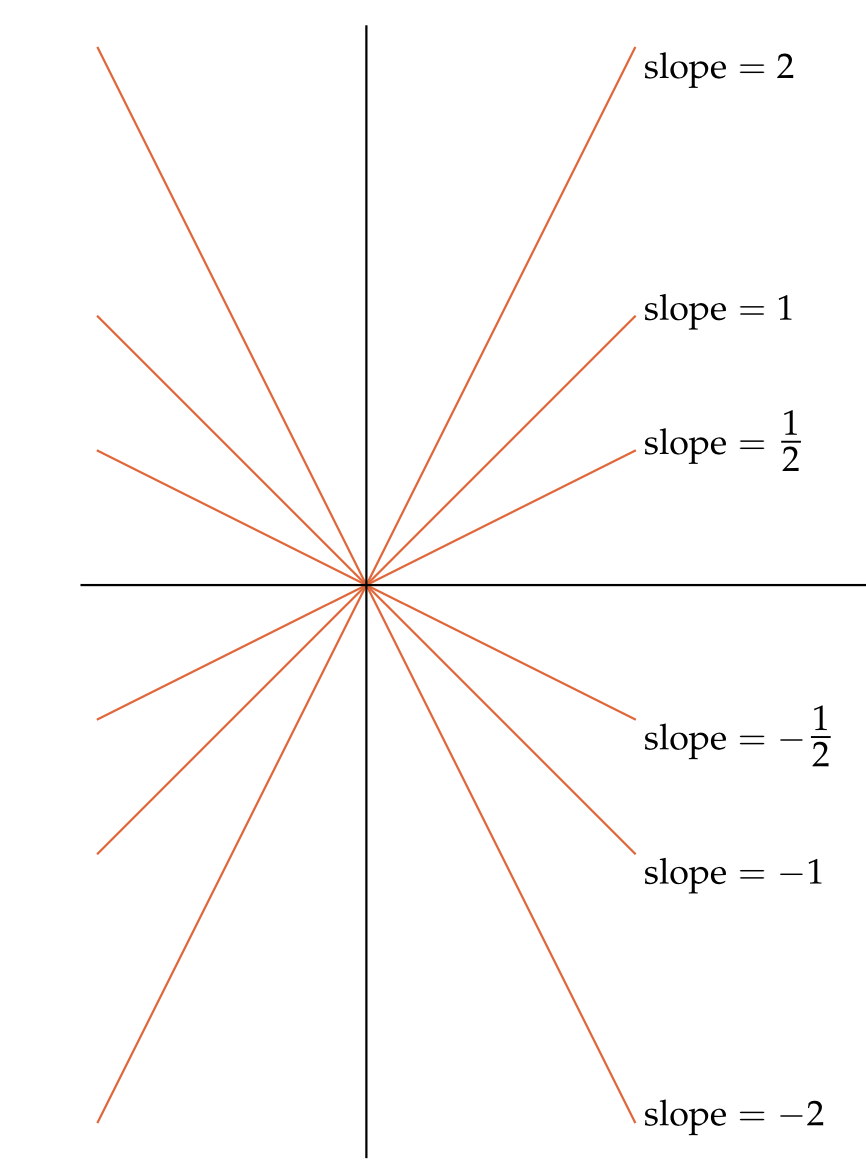
\includegraphics[width=0.5\linewidth]{slope2.png}
\end{figure}
\textbf{Key Points:}
\begin{itemize}
    \item Positive slope slands up from left to right
    \item Negative slope slands down from left to right
    \item Horizontal line has slope = 0
    \item Vertical line has no slope
\end{itemize}

\subsection{Line Equation}
\subsubsection{Slope and one point on it}
The line in the xy-plane that has slope \(m\) and contains the point \((x1, y1)\) is given by the equation
\[y - y_{1} = m(x  -  x_{1})\]
\begin{figure}
  \centering
  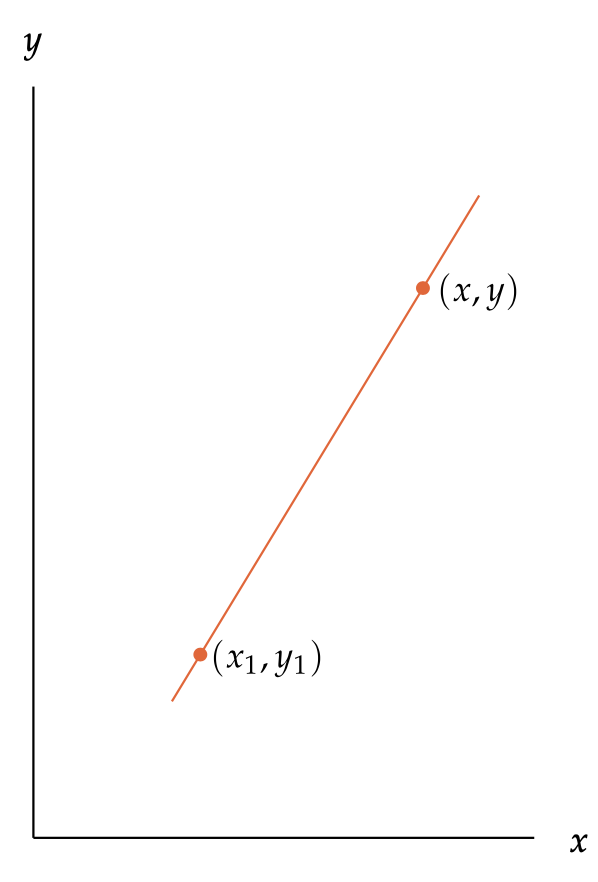
\includegraphics[width=0.5\linewidth]{line1.png}
\end{figure}

\subsubsection{Slope and \(y\) intercept}
The line in the xy-plane with slope \(m\) that intersects the \(y\) axis at \(0,b\) is given by the equation
\[y = mx+b\]
\begin{figure}
  \centering
  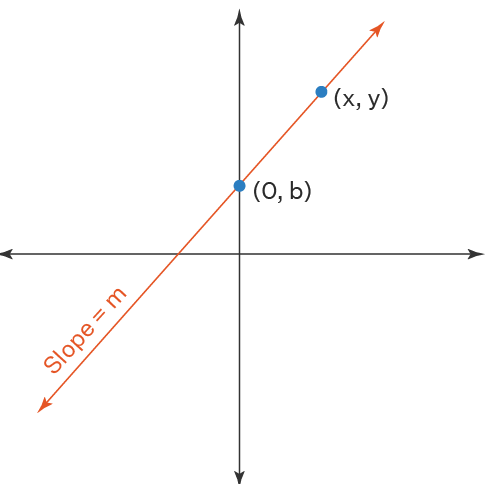
\includegraphics[width=0.5\linewidth]{line2.png}
\end{figure}

The line in the xy-plane that contains the points \(x_{1},y_{1}\) and \(x_{2}, y_{2}\) where \(x_{1} \neq x_{2}\), is
\[y-y_{1} = \left( \frac{y_{2} - y_{1}}{x_{2} - x_{1}} \right) (x-x_{1})\]

\subsection{Linear Function}
A \textbf{linear function} is a function \(f\) of the form
\[f(x) = mx + b\]
where \(m\) and \(b\) are numbers.

\subsubsection{Linear Functions: Origin vs Y-Intercept}
\textbf{Example 1: Temperature Conversion}
\begin{itemize}
    \item Correct formula: \( F = 1.8C + 32 \) (Starts at 32°F)
    \item Incorrect direct proportion: \( F' = 1.8C \) (Wrong assumption)
\end{itemize}
\textbf{Example 2: Weight Conversion}
\begin{itemize}
    \item True conversion: \( lb = 2.205 \times kg \) (Passes through origin)
    \item Shipping charge model: \( lb' = 5 + 2.205 \times kg \) (Has minimum billable weight or fixed cost markup)
\end{itemize}
\begin{figure}
\centering
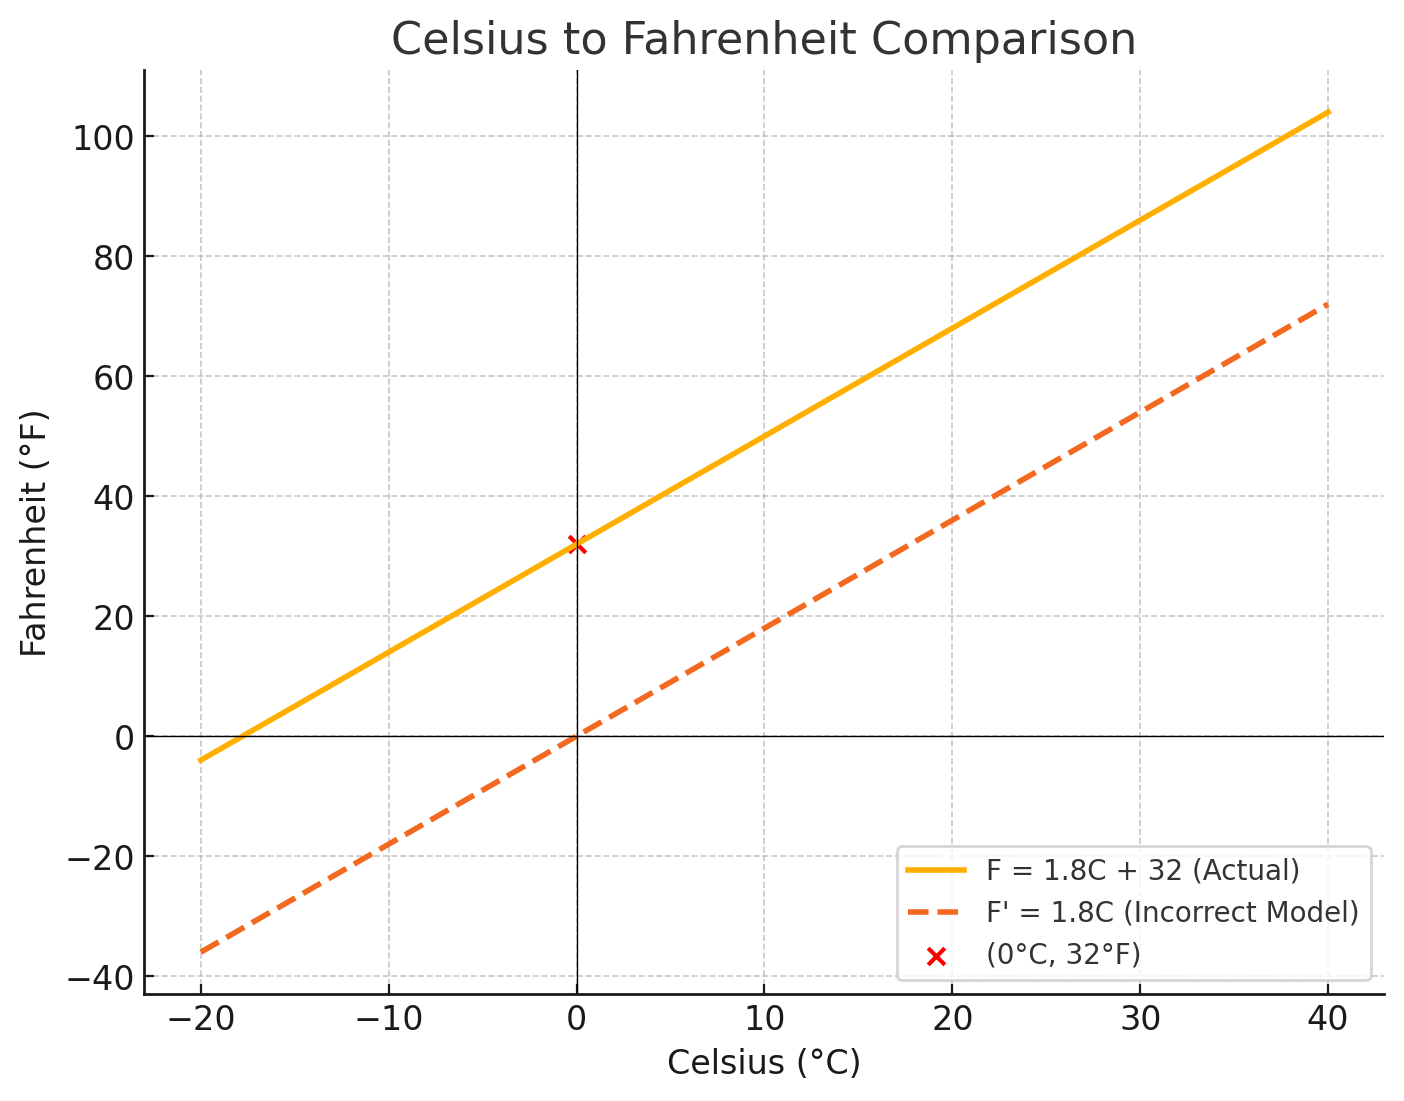
\includegraphics[width=0.45\linewidth]{Celsius to Fahrenheit Comparison.png}
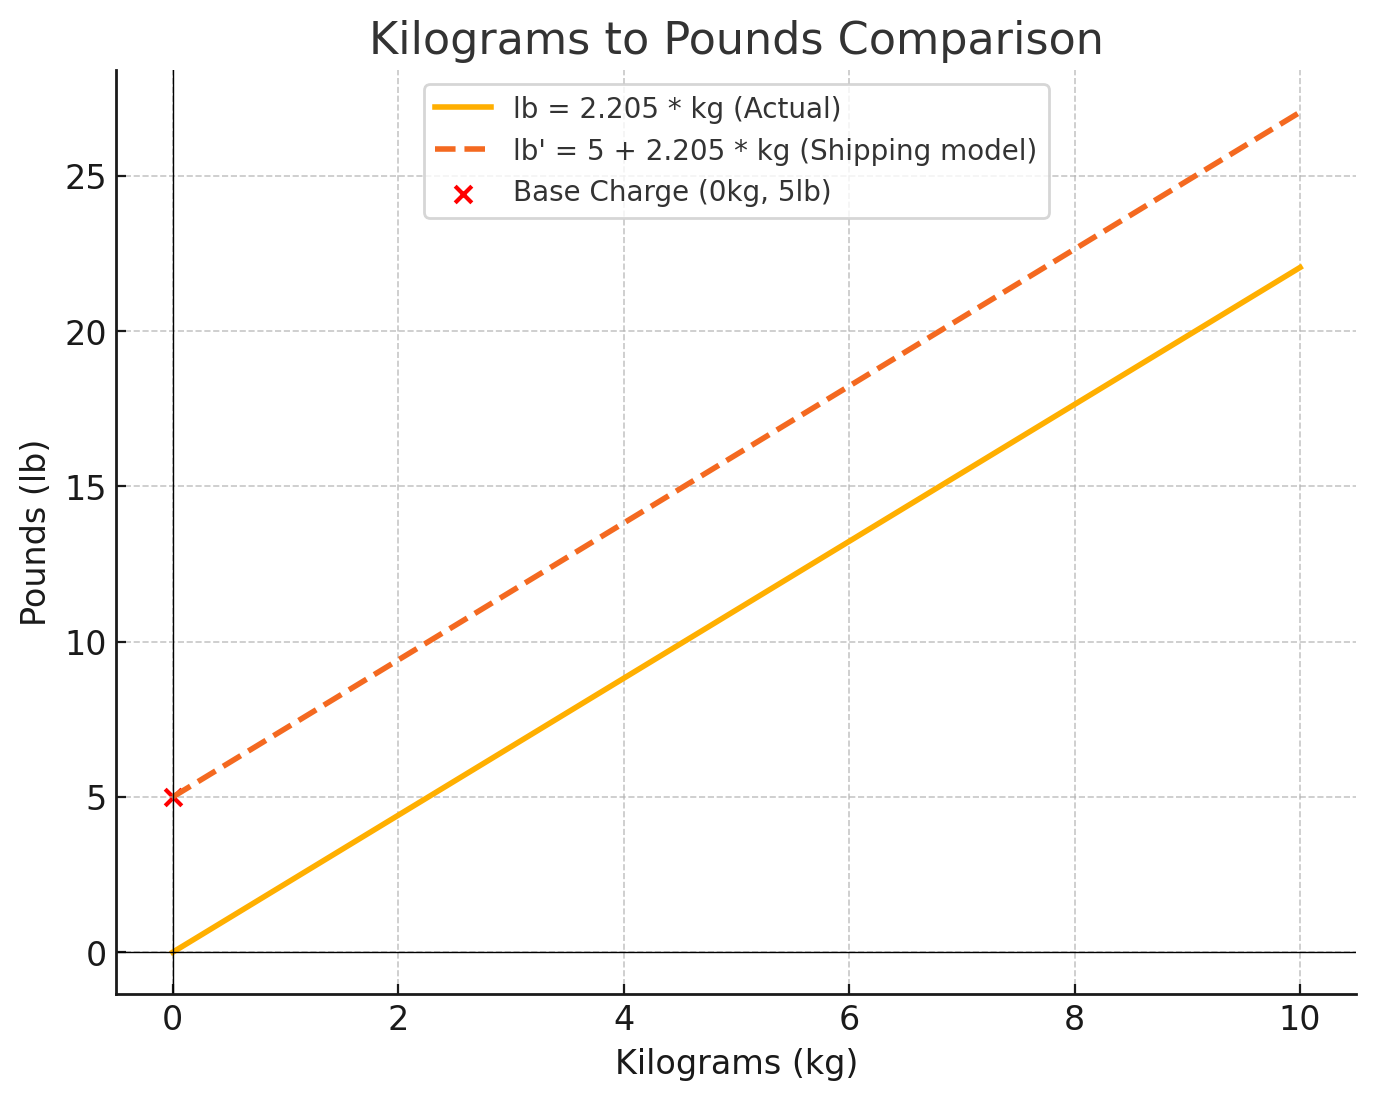
\includegraphics[width=0.45\linewidth]{Kilograms to Pounds Comparison.png}
\end{figure}

\subsection{Constant Function}
A constant function is a function \(f\) of the form \(f (x) = b\),  where \(b\) is a number.
\begin{figure}
\centering
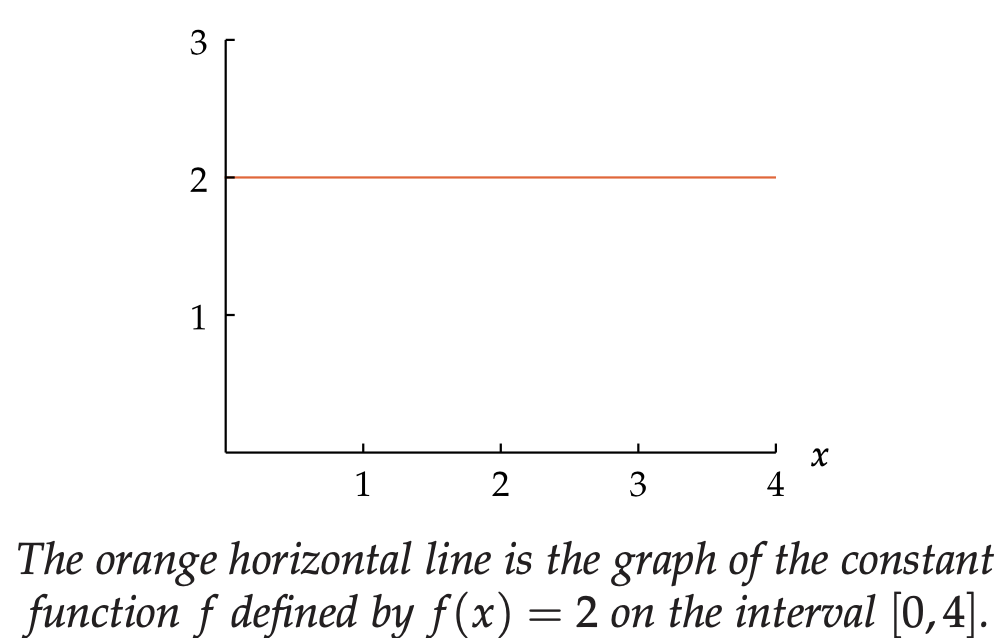
\includegraphics[width=0.6\linewidth]{constant.png}
\end{figure}

\subsection{Parallel Lines}
\begin{figure}
  \centering
  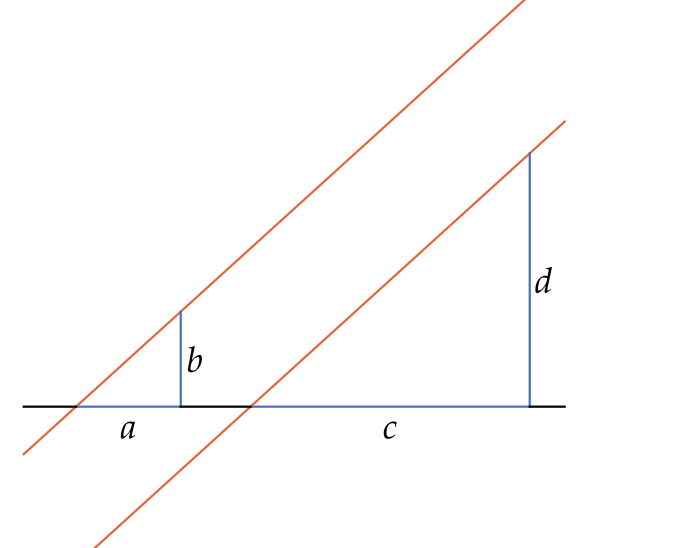
\includegraphics[scale=0.2]{parallel.png}
\end{figure}
As two lines are parallel, the corresponding angles are concurent and so two triangles are similar so
\[\frac{a}{c} = \frac{b}{d} \implies \frac{b}{a} = \frac{d}{c}  \]
it has same slope.

\subsection{Negative Slope}
\begin{figure}
  \centering
  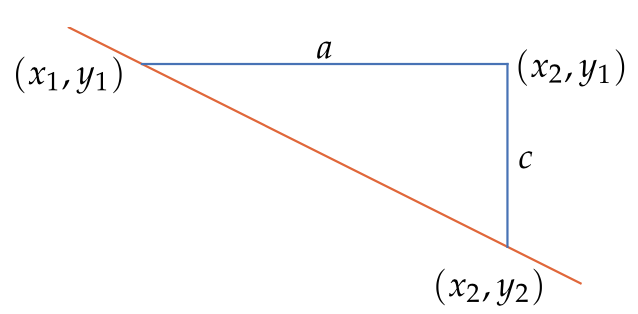
\includegraphics[scale=0.3]{negative-slope.png}
\end{figure}
As lengths are positive \(a = x_{2} - x_{1}\) and \(c = y_{1} - y_{2} \)
Slope  = \(\frac{y_{2} - y_{1}}{x_{2} - x_{1}} = -\frac{c}{a} \

\subsection{Perpendicular Lines}
\begin{figure}
  \centering
  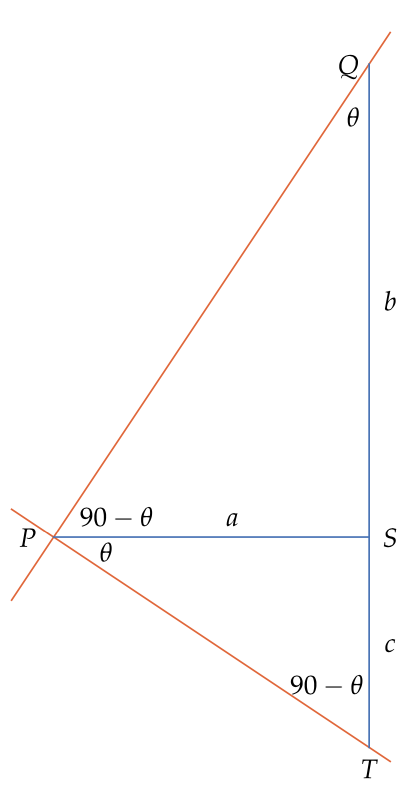
\includegraphics[width=0.5\linewidth]{perpendicular.png}
\end{figure}
\(\triangle PSQ \) and \( \triangle TSP \) are similar
\(\frac{QS}{SP} = \frac{PS}{ST} \implies \frac{b}{a} = \frac{a}{c} \
Multiplying by \(-\frac{c}{a} \implies \frac{b}{a} \cdot \left( - \frac{c}{a} \right) = -1  \

\subsection{Unequal Scales}
Angles are distorted by unequal scales on coordinate axes. In graphs with unequal scales on the two coordinate axes, angles are not accurately represented.
\begin{figure}
  \centering
  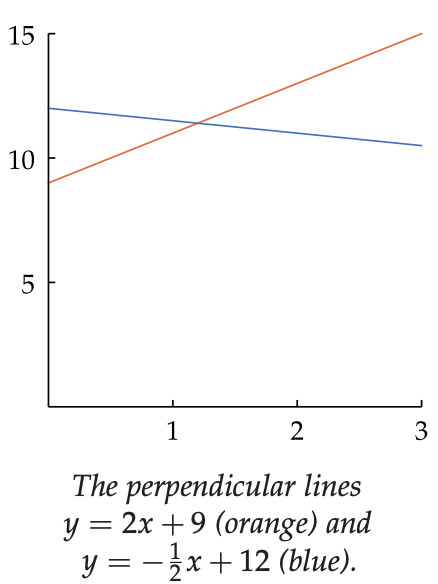
\includegraphics[scale=0.25]{unequal-scale.png}
\end{figure}

\section{Quadratic Functions and Conics}
\subsection{Conics}
\begin{figure}
  \begin{center}
    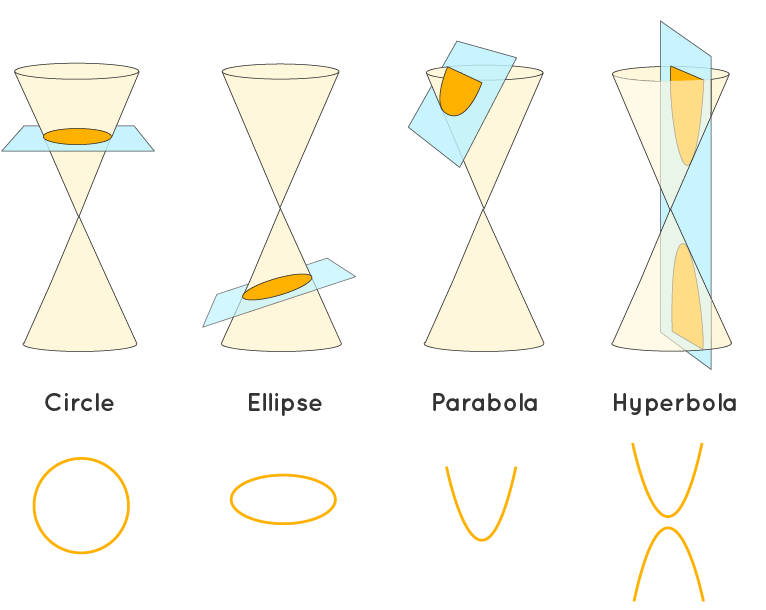
\includegraphics[scale = 0.3]{conic-section.png}
  \end{center}
\end{figure}

\subsection{Quadratic Function}
The function of the form
\[ax^{2} + bx + c = 0\]
where \(a,b,c\) are real numbers with \(a \neq 0\)
\begin{itemize}
    \item if \(b^{2} - 4ac < 0\), then equation have no real solutions
    \item if \(b^{2} - 4ac = 0\), then equation has one solution, \(x = -\frac{b}{2a}\)
    \item if \(b^{2} - 4ac  > 0\), then equation has two solutions \(x = \frac{-b \underset{-}{+}\sqrt{b^{2} - 4ac}}{2a}
\end{itemize}

\subsection{Parabola}
A \textbf{parabola} is the graph of a quadratic function. The \textbf{vertex} of the parabola is the where the line of symmetry of the parabola, intersects the parabola.
Suppose \(f\) is a quadratic function. Complete the square to write \(f\) in the form
\[ f(x) = a(x-h)^{2} + k \
\begin{itemize}
    \item If \(a > 0\) then \(f(x)\) attains its minimum value \(k\) when \(x=h\) and the graph of \(f\) is a parabola that opens upward.
    \item If \(a < 0 \) then \(f(x) \) its maximum value \(k\) when \(x=h\) and the graph of \(f\) is a parabola that opens downward
    \item The vertex of the graph is \(h,k\)
\end{itemize}

\subsubsection{Example}
\[f(x) = -3x^{2} + 12x - 8 \
\begin{enumerate}
  \item For what value of \(x\) does \(f (x) \) attain its maximum value?
  \item What is the maximum value of \(f (x)\)?
  \item Find the vertex
\end{enumerate}
Sol:
\[f(x) = -3x^{2} + 12x - 8 \implies -3(x^{2} - 4x + 4) + 4 \implies -3(x-2)^{2} + 4 \
\begin{enumerate}
\item \(x = 2\
\item \(f(x=2) = 4\
\item \( (2,4) \
\end{enumerate}

\begin{figure}
\centering
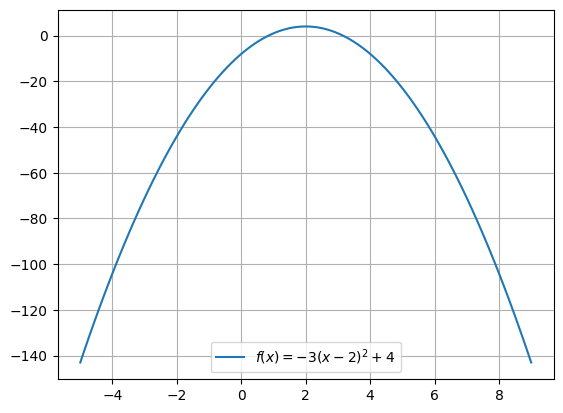
\includegraphics[scale=0.6]{parabola.png}
\end{figure}

\subsection{Distance Between Points}
\begin{figure}
\centering
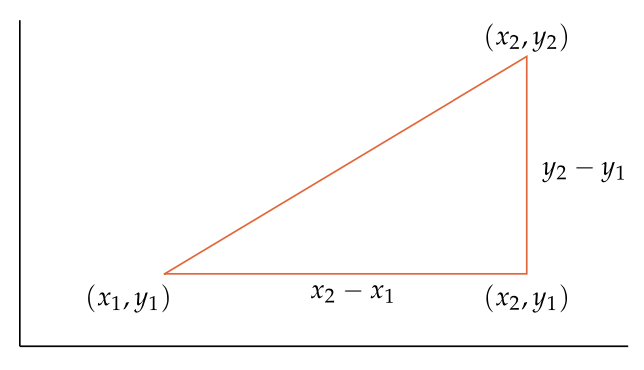
\includegraphics[scale=0.3]{distance-between-points.png}
\end{figure}
The distance between points \(x_{1}, y_{1}\) and \(x_{2}, y_{2}\) is given by
\[\sqrt{ \left(x_{2} - x_{1} \right)^{2}  + \left( y_{2} - y_{1} \right)^{2} }\]

\subsection{Circle}
The circle with center \(h,k\) and radius \(r\) is the set of the points \(x,y\) that satisfy the equation
\[\left(x-h\right)^{2} + \left(y-k\right)^{2} = r^{2}\]

\subsection{Ellipse}
\begin{figure}
\centering
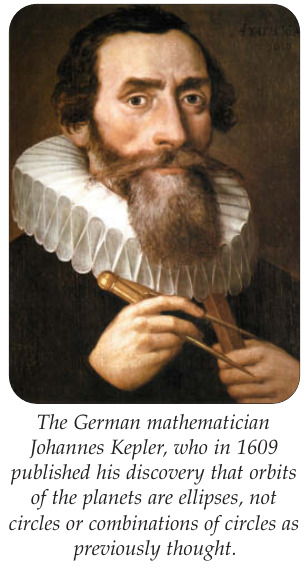
\includegraphics[scale=0.38]{ellipse0.png}
\end{figure}

Stretching the circle horizontally and/or vertically produces a curve called an \textbf{ellipse}.
\begin{figure}
\centering
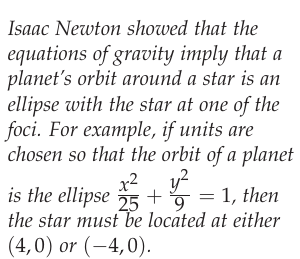
\includegraphics[scale=0.4]{ellipse1.png}
\end{figure}

\subsubsection{Example}
Equation of the circle is given by \(u^{2} + v^{2} = 1\).
By stretching \(x = 3u, y = 5v\),
Substituting for \(u,v\)
\[ \left( \frac{x}{3} \right)^{2} + \left(\frac{y}{5}\right)^{2} = 1 \

\subsubsection{Ellipse Equation}
\[\frac{x{2}}{a^{2}} + \frac{y^{2}}{b^{2}} = 1 \
The \textbf{foci} of an ellispe are two points with the property that the sum of the distances from the \textbf{foci} to any point on the ellipse is a constant independent of the point on the ellispe.

\begin{figure}
\centering
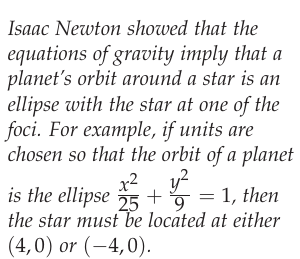
\includegraphics[scale=0.5]{ellipse1.png}
\end{figure}

\begin{figure}
\centering
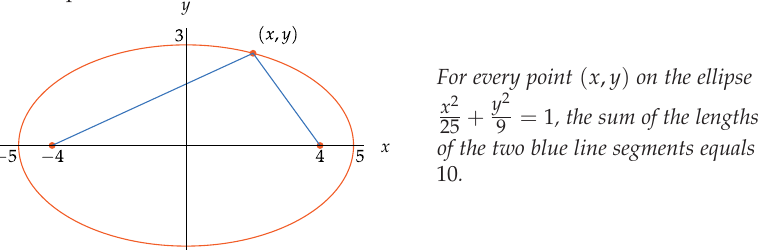
\includegraphics[scale=0.4]{foci.png}
\end{figure}

\subsection{Eccentricity of an Ellipse}
The \textbf{eccentricity} (\(e\)) of an ellipse is a measure of how much the ellipse deviates from being a circle. It is defined as
\[ e = \frac{c}{a} .
\qquad c^2 = a^2 - b^2, 
\qquad e = \sqrt{1 - \frac{b^2}{a^2}}\]
where:
\begin{itemize}
    \item \(c\) is the distance from the center to a focus.
    \item \(a\) is the length of the semi-major axis.
\end{itemize}
Additionally, the semi-minor axis \(b\) is related to \(a\) and \(c\) by:
\textbf{Key Points:}
\begin{itemize}
    \item If \(e = 0\), the ellipse is a circle.
    \item If \(0 < e < 1\), the ellipse is elongated, with greater elongation as \(e\) increases.
\end{itemize}

\subsection{Hyperbola}
The graph of the equation of the form
\[ \frac{y^2}{b^2} - \frac{x^2}{a^2} = 1 \
where \(a,b\) are non-zero numbers.
\begin{figure}
\centering
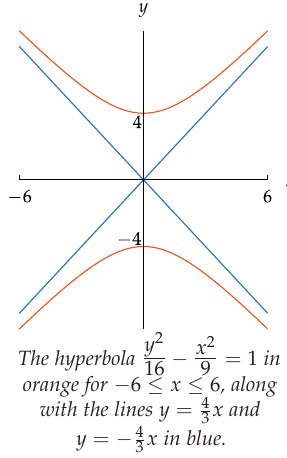
\includegraphics[scale=0.5]{hyperbola2.png}
\end{figure}

The foci of a hyperbola are two points with the property that the difference of the distances from the foci to a point on the hyperbola is a constant independent of the point on the hyperbola.
\begin{figure}
\centering
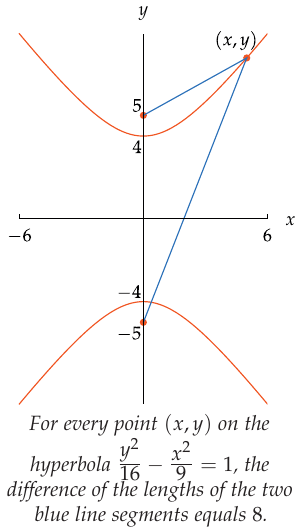
\includegraphics[scale=0.4]{hyperbola3.png}
\end{figure}
\begin{figure}
\centering
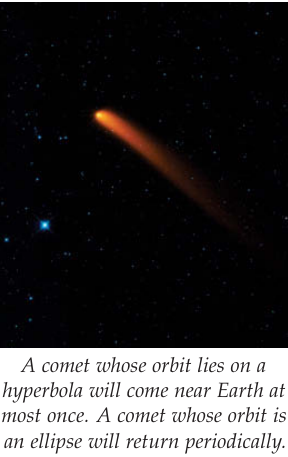
\includegraphics[scale=0.5]{hyperbola1.png}
\end{figure}

\section{Exponents}
\subsection{Positive Integer Exponent}
If \(x\) is a real number and \(m\) is a positive integer, then \(x^{m}\) is defined to be the product with \(x\) appearing \(m\) times
\[x^{m} = \underset{x \;	ext{appears}\;	ext{m} \;	ext{times}}{\underbrace{x \cdot x \cdots x }}\]

\subsubsection{Properties}
Suppose \(x\) and \(y\) are numbers and \(m\) and \(n\) are positive integers. Then
\[x^{m}x^{n} = x^{m+n} \
\left(x^{m}\right)^{n} = x^{mn} \
x^{m}y^{m} = \left(xy\right)^{m}\]

\subsection{\(x^{0}\)}
If  \(x^{m}x^{n} = x^{m+n}\) then we can write \(x^{0}x^{n} = x^{0+n} = x^{n} \implies x^{0} = 1\;for\;	ext{x} \neq 0\]

\subsubsection{What is \(0^{0}\)}
\begin{itemize}
  \item The rule \( x^0 = 1 \) (for \( x \neq 0 \)) suggests that \( 0^0 \) should be \(1\).
  \item The rule \( 0^m = 0 \) (for \( m > 0 \)) suggests that \( 0^0 \) should be \(0\).
  \item Since these two rules contradict each other, \( 0^0 \) is left undefined in general mathematics.
  \item However, in combinatorics and programming, \( 0^0 \) is often defined as \(1\) for convenience.
\end{itemize}

\subsection{Negative Integer Exponents}
If \(x^{m}x^{n} = x^{m+n}\), if we take \(m = -n \), then
\[x^{m}x^{-m} = x^{0} = 1 \implies x^{m}x^{-m} = 1\]
We have to define \(x^{-m}\) to equal the multiplicative inverse of \(x^{m}\).
If \(x \neq 0\) and \(m\) is a positive integer, then \(x^{-m}\) is defined to multiplicative inverse of \(x^{m}\)
\[x^{-m} = \frac{1}{x^{m}}\]

\subsubsection{Exponents: Some Graphs}
\begin{figure}
\centering
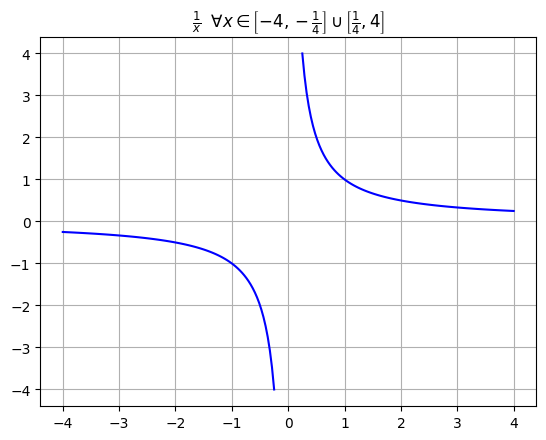
\includegraphics[scale=0.4]{exponent-graph1.png}
\caption{graph of \(\frac{1}{x}\)}
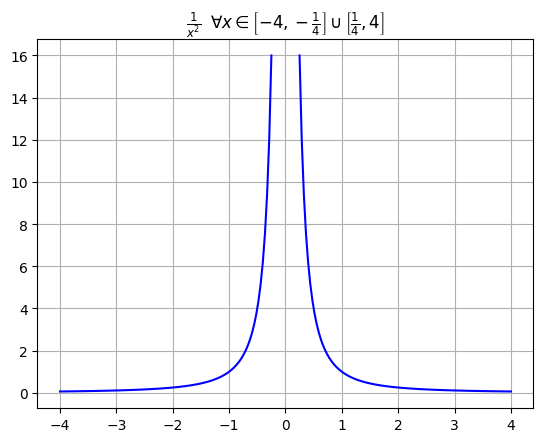
\includegraphics[scale=0.4]{exponent-graph2.png}
\caption{graph of \(\frac{1}{x^{2}}\)}
\end{figure}

\subsubsection{Graph of Negative Integer Exponents}
if \(m\) is  a positive integer then
\begin{itemize}
  \item \(\frac{1}{x^{m}}\) behaves like \(\frac{1}{x}\) if \(m\) is odd
  \item \(\frac{1}{x^{m}}\) behaves like \(\frac{1}{x^{2}}\) if \(m\) is even
  \item Larger values of \(m\) correspond to functions whose graphs get closer to the x-axis more rapidly for large values of \(x\) and closer to the vertical axis more rapidly for values of \(x\) near 0
\end{itemize}

\subsection{Roots}
\subsubsection{\(m^{th}\) root}
If \(m\) is a positive integer and \(x\) is a real number, then \(x^{m}\) is defined to be the real number satisfying the equation
\[\left(x^{m}\right)^{m} = x \
subject to the following conditions:
\begin{itemize}
\item  If \(x < 0\) and \(m\) is an even integer, then \(x^{m} \)is undefined
\item If \(x > 0\) and \(m\) is an even integer, then \(x^{m} \)is chosen to be the \textit{\textcolor{red}{positive number}} satisfying the equation above
\end{itemize}
The number \(x^{m}\) is called the \textbf{\(m^{th}\)} root of \(x\).

\subsubsection{Example}
\begin{itemize}
  \item \(8^{3}\) and \(-8^{3}\)
  \item \(9^{2}\) and \(-9^{2}\)
\end{itemize}
Solution:
\begin{enumerate}
  \item \( \left(8^{3}\right)^{3} = 8 \implies 2 \
  \item \( \left(-8^{3}\right)^{3} = -8 \implies -2 \). There is no other number other than \(-2\)
  \item \( \left( 9^{2} \right)^{2} = -3 \; or \;3\). But as per the rule, we have to choose positive possibility, that is \(3\
  \item \( \left( -9^{2} \right)^{2} \). No number real number exists so no solution
\end{enumerate}

\subsection{Rational Exponents}
Suppose \(\frac{n}{m}\) is a fraction in reduced form, where \(n\) and \(m\) are integers and \(m > 0\). Then, whenever it makes sense,
\[ x^{\frac{n}{m}} = \Bigl(x^{\frac{1}{m}}\Bigr)^n. \
\textbf{Note:} For the expression \(x^{\frac{1}{m}}\) to be defined, additional conditions on \(x\) may be required (for example, if \(m\) is even, then typically \(x \ge 0\)).

\subsection{Algebra of Exponents}
Let \(p, q\) be rational numbers and \(x, y\) be positive numbers. Then the following rules hold:
\begin{itemize}
  \item \(x^p \cdot x^q = x^{\,p+q}
  \item \(x^p \cdot y^p = (xy)^p
  \item \((x^p)^q = x^{\,pq}
  \item \(x^0 = 1
  \item \(x^{-p} = \dfrac{1}{x^p}
  \item \(\dfrac{x^p}{x^q} = x^{\,p-q}
  \item \(\left(\dfrac{x}{y}\right)^p = \dfrac{x^p}{y^p}
\end{itemize}

\section{Polynomials}
\subsection{Polynomial Definition}
A polynomial is a function \( p \) such that
\[ p(x) = a_0 + a_1 x + a_2 x^2 + \cdots + a_n x^n, \
where \( n \) is a nonnegative integer and \( a_0, a_1, a_2, \dots, a_n \) are numbers.

\subsection{Degree of a Polynomial}
Suppose \( p \) is a polynomial defined by
\[ p(x) = a_0 + a_1 x + a_2 x^2 + \cdots + a_n x^n. \
If \( a_n \neq 0 \), then we say that \( p \) has degree \( n \). The degree of \( p \) is denoted by \(\deg p\).

\subsection{Polynomial Graphs}
\begin{figure}
\centering
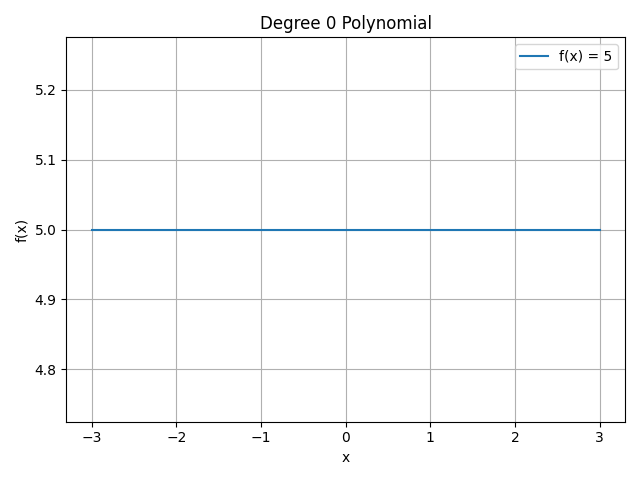
\includegraphics[width=0.45\linewidth]{polynomial_degree_0.png}
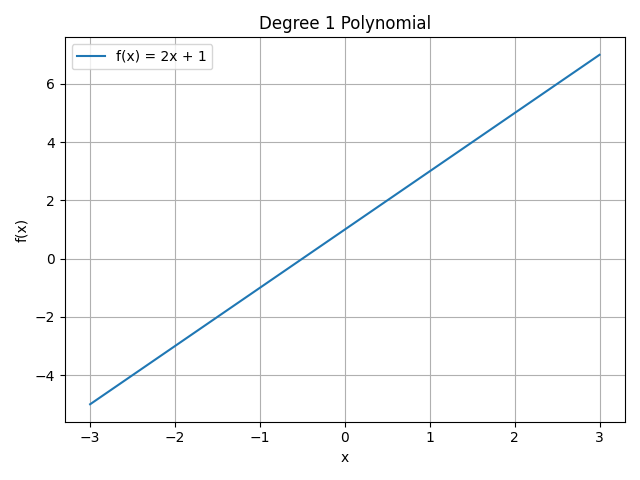
\includegraphics[width=0.45\linewidth]{polynomial_degree_1.png}
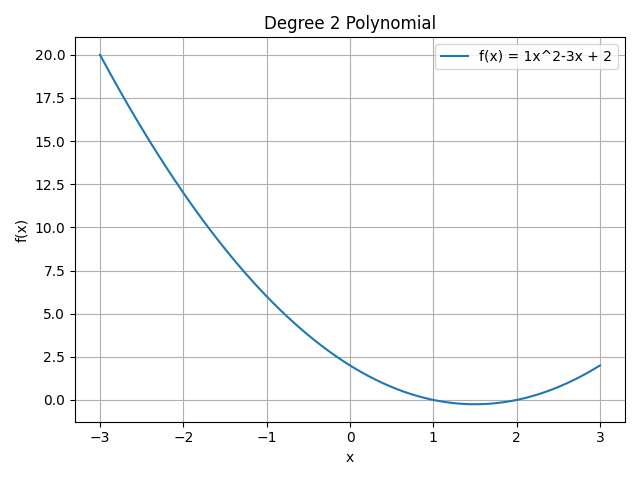
\includegraphics[width=0.45\linewidth]{polynomial_degree_2.png}
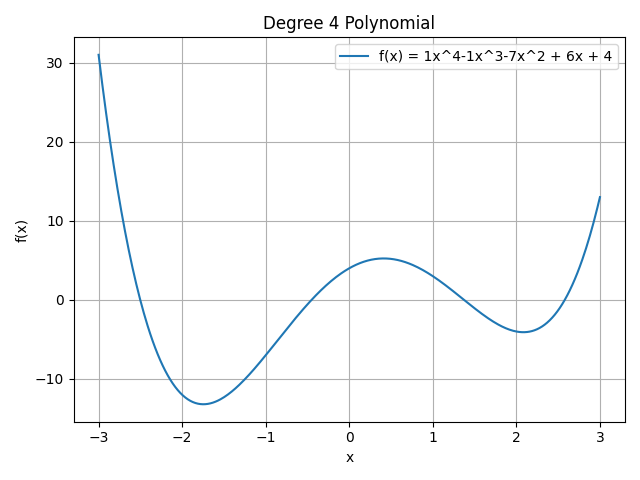
\includegraphics[width=0.45\linewidth]{polynomial_degree_4.png}
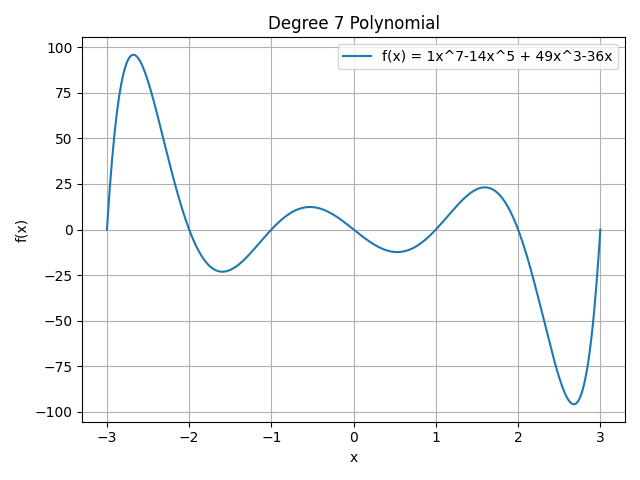
\includegraphics[width=0.45\linewidth]{polynomial_degree_7.png}
\end{figure}

\subsection{The Algebra of Polynomials}
Two functions can be added, subtracted, or multiplied, producing another function. Specifically, if \(p\) and \(q\) are functions, then the functions
\[ p+q,\quad p-q,\quad \text{and} \quad pq \
are defined by
\[ (p+q)(x) = p(x) + q(x), \
\[ (p-q)(x) = p(x) - q(x), \
\[ (pq)(x) = p(x) \, q(x). \

\subsection{Degree of the Sum and Difference of Two Polynomials}
If \(p\) and \(q\) are nonzero polynomials, then
\[ \deg(p+q) \leq \max\{\deg p,\, \deg q\}, \
and
\[ \deg(p-q) \leq \max\{\deg p,\, \deg q\}. \

\subsection{Degree of the Product of Two Polynomials}
If \(p\) and \(q\) are nonzero polynomials, then
\[ \deg(pq) = \deg p + \deg q. \

\subsection{Example: Polynomials \(p\) and \(q\)}
Suppose \(p\) and \(q\) are polynomials defined by
\[ p(x) = 2 - 3x^2 \quad \text{and} \quad q(x) = 4x + 7x^5. \
Answer the following:
\begin{enumerate}
    \item What is \(\deg p\)?
    \item What is \(\deg q\)?
    \item Find a formula for \(pq\).
    \item What is \(\deg(pq)\)?
\end{enumerate}
Solution:
\begin{enumerate}
    \item Since \(p(x) = 2 - 3x^2\) has the highest power \(x^2\), we have \(\deg p = 2\).
    \item For \(q(x) = 4x + 7x^5\), the highest power is \(x^5\), so \(\deg q = 5\).
    \item The product \(pq\) is computed as follows:
    \[ pq = (2-3x^2)(4x+7x^5) = 2\cdot 4x + 2\cdot 7x^5 - 3x^2\cdot 4x - 3x^2\cdot 7x^5, \
    which simplifies to:
    \[ pq = 8x - 12x^3 + 14x^5 - 21x^7. \
    \item The highest power in \(pq\) is \(x^7\), so \(\deg(pq) = 7\).
\end{enumerate}

\subsection{Roots of a Function}
A number \(t\) is called a zero of a function \(p\) if
\[ p(t) = 0. \

\subsection{Closed-Form Expression}
A closed-form expression is an explicit formula that can be written using a finite number of standard operations and functions (e.g., addition, multiplication, exponentiation, logarithms, trigonometric functions). It does not involve infinite series, integrals, or iterative processes.
\textbf{Example:} The quadratic formula,
\[ x = \frac{-b \pm \sqrt{b^2-4ac}}{2a}, \
is a closed-form expression.

\subsection{Zeros of Higher–Degree Polynomials}
\begin{itemize}
  \item The quadratic formula gives exact zeros for degree–2 polynomials.
  \item Although formulas exist for cubics and quartics, they are rarely used.
  \item No closed-form formula exists for polynomials of degree 5 or higher.
  \item Numerical methods can approximate zeros for any polynomial.
  \item \textbf{Example:} For
  \[ p(x)=x^5-5x^4-6x^3+17x^2+4x-7, \
  approximate zeros are:
  \[ -1.80,\; -0.73,\; 0.63,\; 1.48,\; 5.56. \
\end{itemize}

\subsubsection{Zeros on graph}
\begin{figure}
\centering
\includegraphics[scale=0.23]{zeros.png}
\end{figure}
\begin{figure}
\centering
\includegraphics[scale=0.3]{no-real-zeros.png}
\caption{The function \(x^{2}+1\) has no real zeros}
\end{figure}

\subsection{Factor of a Polynomial}
Suppose \(p\) is a polynomial and \(t\) is a real number. Then \(x-t\) is called a \emph{factor} of \(p(x)\) if there exists a polynomial \(G(x)\) such that
\[ p(x) = (x-t)\,G(x) \
for every real number \(x\).

\subsection{Example: Factors and Zeros of a Polynomial}
Let
\[ p(x) = (x-2)(x-5)(x^2+1). \
\begin{enumerate}[(a)]
  \item Explain why \(x-2\) is a factor of \(p(x)\).
  \item Explain why \(x-5\) is a factor of \(p(x)\).
  \item Show that \(2\) and \(5\) are zeros of \(p\).
  \item Show that \(p\) has no (real) zeros except \(2\) and \(5\).
\end{enumerate}
Solution:
\begin{enumerate}[(a)]
  \item The polynomial is given in factored form as \((x-2)(x-5)(x^2+1)\). Since \((x-2)\) appears as one of the factors, it is a factor of \(p(x)\).
  \item Similarly, \((x-5)\) appears explicitly in the factorization, so it is a factor of \(p(x)\).
  \item To show that \(2\) and \(5\) are zeros, substitute:
    \[ p(2) = (2-2)(2-5)(2^2+1) = 0\cdot(-3)\cdot5 = 0, \
    \[ p(5) = (5-2)(5-5)(5^2+1) = 3\cdot0\cdot26 = 0. \
    Thus, \(p(2)=0\) and \(p(5)=0\).
  \item The factor \(x^2+1\) yields \(x^2=-1\), which has no real solutions. Hence, aside from the zeros from \((x-2)\) and \((x-5)\), there are no other real zeros.
\end{enumerate}

\subsection{Zeros and Factors of a Polynomial}
Suppose \(p\) is a polynomial and \(t\) is a real number. Then \(t\) is a zero of \(p\) if and only if \(x-t\) is a factor of \(p(x)\).

\subsection{Number of Zeros of a Polynomial}
A nonzero polynomial \(p(x)\) of degree \(n\) has at most \(n\) zeros.
A polynomial of degree 15 has at most 15 zeros. This is because each (real) zero \(t_j\) of a polynomial \(p\) corresponds to a factor \((x-t_j)\) in a factorization of the form
\[ p(x) = (x-t_1)(x-t_2)\cdots(x-t_m) \, G(x), \
where \(G(x)\) is a polynomial with no (real) zeros. If \(p(x)\) had more than 15 zeros, then the right-hand side would represent a polynomial of degree higher than 15, contradicting the fact that \(p\) is of degree 15.

\subsection{Behavior of a Polynomial Near \(\pm\infty\)}
\begin{itemize}
  \item \textbf{\(x\) near \(+\infty\):} \(x\) is very large.
  \item \textbf{\(x\) near \(-\infty\):} \(x\) is very negative (i.e., \(|x|\) is very large).
  \item Our goal is to determine whether a polynomial \(p(x)\) is positive or negative in these extremes.
\end{itemize}
\begin{figure}
\centering
\includegraphics[scale=0.2]{at-infty.png}
\end{figure}
To analyze the behavior as \(x\to\pm\infty\), factor out the highest degree term.
If \(c\,x^n\) is the highest degree term in \(p(x)\), then for very large \(|x|\), \(p(x)\) behaves like \(c\,x^n\).

\subsection{Zero in an Interval}
\subsubsection{Intermediate Value Theorem}
Suppose \(p\) is a polynomial and \(a, b \in \mathbb{R}\) with \(a < b\). If \(p(a)\) and \(p(b)\) have opposite signs, then there exists a number \(c \in (a, b)\) such that \(p(c)=0\).

\subsection{Example 7: Zero in an Interval}
Let
\[ p(x) = x^5 + x^2 - 1. \
Explain why \(p\) has a zero in the interval \((0,1)\).
Solution:
Evaluate the polynomial at the endpoints:
\[ p(0) = 0^5 + 0^2 - 1 = -1 \quad \text{and} \quad p(1) = 1^5 + 1^2 - 1 = 1. \
Since \(p(0) < 0\) and \(p(1) > 0\), by the Intermediate Value Theorem, there exists a \(c \in (0,1)\) such that \(p(c)=0\).

\subsection{Zeros for Polynomials with Odd Degree}
Every polynomial with odd degree has at least one real zero.
For a polynomial \(p(x)\) of odd degree, as \(x \to -\infty\), \(p(x)\) tends to \(-\infty\) (or \(+\infty\)) and as \(x \to \infty\), \(p(x)\) tends to \(+\infty\) (or \(-\infty\)).
By the Intermediate Value Theorem, since \(p(x)\) changes sign, there exists at least one real number \(c\) such that \(p(c)=0\).

\section{Rational Function}
\subsection{Definition}
A \emph{rational function} is a function \(r\) defined by
\[ r(x) = \frac{p(x)}{q(x)}, \
where \(p(x)\) and \(q(x)\) are polynomials, with \(q(x) \neq 0\).

\subsection{Domain of a Rational Function & Example for \(r(x)\)}
The domain of a rational function
\[ \frac{p(x)}{q(x)} \
is the set of all real numbers where the expression makes sense. Since division by 0 is undefined, we exclude all zeros of \(q(x)\).

\subsubsection{Example}
\[r(x)=\frac{3x^5+x^4-6x^3-2}{x^2-9}\]
Factor the denominator:
\[ x^2-9=(x-3)(x+3). \
Thus, \(r(x)\) is undefined at \(x=3\) and \(x=-3\). Hence, its domain is
\[ \{x\in\mathbb{R}: x\neq 3 \text{ and } x\neq -3\}. \

\subsubsection{Example}
\[s(x)=\frac{x^3-6x+5}{x^4+9}\]
The denominator \(x^4+9\) is always positive (since \(x^4\ge 0\) and \(9>0\)). Therefore, \(s(x)\) is defined for every real number.
Domain of \(s(x)\) :
\( \mathbb{R} \

\subsection{Advantages of Mixed Representation}
Expressing a rational function as a polynomial plus a proper rational function (one where the numerator's degree is less than the denominator's) is analogous to writing an improper fraction as an integer plus a proper fraction.
\begin{itemize}
  \item \textbf{Simplification:} It makes further operations (such as integration, differentiation, and partial fraction decomposition) easier.
  \item \textbf{Asymptotic Insight:} The polynomial part reveals the behavior of the function as \(x\to\pm\infty\), while the proper fraction (the remainder) tends to zero for large \(|x|\).
  \item \textbf{Clarity:} It separates the "whole" part from the "fractional" part, making the function's structure more transparent.
\end{itemize}

\subsection{Mixed Rational Function Representation}
Express
\[ \frac{x^5 + 6x^3 + 11x + 7}{x^2+4} \
in the form
\[ G(x) + \frac{ax+b}{x^2+4}, \
where \(G(x)\) is a polynomial and \(a, b\) are constants.

\subsection{Procedure for Dividing Polynomials}
\begin{enumerate}
  \item \textbf{Rewrite:} Express the highest-degree term in the numerator as a single term times the denominator, plus the necessary adjustment.
  \item \textbf{Simplify:} Use the rewritten numerator to simplify the quotient.
  \item \textbf{Iterate:} Repeat steps (1) and (2) on the remaining rational function until the degree of the numerator is less than the degree of the denominator or the numerator becomes 0.
\end{enumerate}

\subsection{Mixed Representation Example}
Express
\[ \frac{x^5+6x^3+11x+7}{x^2+4} \
in the form
\[ G(x)+\frac{ax+b}{x^2+4}, \
where \(G(x)\) is a polynomial and \(a, b\) are constants.
\subsubsection{Step 1: Eliminate the \(x^5\) Term}
Notice that
\[ x^5=x^3(x^2+4)-4x^3. \
Therefore,
\[
\begin{aligned}
  x^5+6x^3 &= x^3(x^2+4)-4x^3+6x^3\\[1mm]
           &= x^3(x^2+4)+2x^3.
\end{aligned}
\]
So we can write:
\[ \frac{x^5+6x^3+11x+7}{x^2+4}=x^3+\frac{2x^3+11x+7}{x^2+4}. \

\subsubsection{Step 2: Eliminate the \(2x^3\) Term}
Write
\[ 2x^3=2x(x^2+4)-8x. \
Then,
\[
\begin{aligned}
  2x^3+11x+7 &= 2x(x^2+4)-8x+11x+7\\[1mm]
              &= 2x(x^2+4)+(3x+7).
\end{aligned}
\]
Thus,
\[ \frac{2x^3+11x+7}{x^2+4}=2x+\frac{3x+7}{x^2+4}. \

\subsubsection{Final Mixed Representation}
Combining the steps, we have:
\[ \frac{x^5+6x^3+11x+7}{x^2+4}=x^3+2x+\frac{3x+7}{x^2+4}. \

\subsection{Division Algorithm for Polynomials}
If \(p(x)\) and \(q(x)\) are polynomials with \(q(x) \neq 0\), then there exist unique polynomials \(G(x)\) and \(R(x)\) such that
\[ \frac{p(x)}{q(x)} = G(x) + \frac{R(x)}{q(x)}, \
where either \(R(x)=0\) or \(\deg R < \deg q\). Equivalently, we can write
\[ p(x)=q(x)G(x)+R(x). \

\subsection{Division by \(x-t\) and Zeros of a Polynomial}
Fix a real number \(t\) and let \(q(x)=x-t\). Since \(\deg q=1\), the remainder \(R(x)\) is a constant \(c\)(Because degree \(R < \)degree \(q\)). Thus, there exist a polynomial \(G(x)\) and a constant \(c\) such that
\[ p(x) = (x-t)G(x) + c. \
Evaluating at \(x=t\) yields \(p(t)=c\), so we can rewrite this as
\[ p(x) = (x-t)G(x) + p(t). \
\(t\) is a zero of \(p\) if and only if \(p(t)=0\), which happens precisely when
\[ p(x)=(x-t)G(x). \

\subsection{Behavior of a Rational Function Near \(\pm\infty\)}
To determine the behavior of a rational function as \(x\to\pm\infty\), factor out the highest power of \(x\) in the numerator and the denominator.
Consider
\[ r(x)=\frac{9x^5-2x^3+1}{x^8+x+1}. \
The highest degree in the numerator is \(x^5\) and in the denominator is \(x^8\). Factoring these out yields:
\[ r(x) \sim \frac{9x^5}{x^8}=\frac{9}{x^3}. \
As \(|x|\) becomes very large:
\begin{itemize}
  \item \(r(x)\to 0\) as \(x\to\infty\) (approaching \(0^+\)).
  \item \(r(x)\to 0\) as \(x\to-\infty\) (approaching \(0^-\)).
\end{itemize}

\subsection{Asymptote of a Rational Function}
A line is an asymptote of a graph if the graph becomes and stays arbitrarily close to the line as \(x\) tends to \(\pm\infty\).
Consider
\[ r(x)=\frac{3x^6-9x^4+6}{2x^6+4x+3}. \
Both the numerator and the denominator are degree 6. Therefore, the horizontal asymptote is the ratio of the leading coefficients:
\[ y=\frac{3}{2}. \
\begin{figure}
\centering
\includegraphics[scale=0.2]{asymptote1.png}
\end{figure}

\subsubsection{Example}
\[ r(x) = \frac{4x^{10}-2x^3+3x+15}{2x^6+x^5+1} \
Solution:
\[ \frac{4x^{10}}{2x^6} = 2x^4. \
Thus, as \(|x|\to\infty\), \(r(x)\) behaves like \(x^{4}\). That is, \(r(x)\) is very large and positive when \( x \to \infty\) and \( x \to -\infty\).

% \chapter{Exponential Functions, Logarithms and e}
\author{Nithin}

\section{Bacterial Growth on the Human Body}
\begin{itemize}
  \item Our skin (and other areas like the mouth, nose, and intestines) hosts hundreds of thousands of microscopic organisms.
  \item In fact, bacterial cells in our body outnumber our own cells.
  \item While some bacteria can cause illness, many are essential for our health.
  \item Bacteria reproduce through binary fission—each cell splits into two.
  \item Under ideal conditions, a single bacterium doubling every hour can lead to over 1,000 cells in 10 hours and more than 16 million in 24 hours.
\end{itemize}

\subsection{Bacterial Growth Over Time}
\begin{table}[ht]
  \centering
  \begin{tabular}{c|ccccccccccc}
    \textbf{Hour} & 0 & 1 & 2 & 3 & 4 & 5 & 6 & 7 & 8 & 9 & 10 \\ \hline
    \textbf{Bacteria} & 1 & 2 & 4 & 8 & 16 & 32 & 64 & 128 & 256 & 512 & 1024 \\
  \end{tabular}
  \caption{Bacterial cell count doubling every hour.}
\end{table}

\section{Population Growth in India}
\begin{itemize}
  \item India is the second most populous country, with about 1.39 billion people in 2021.
  \item Its population grows at an annual rate of roughly 1.2\%.
  \item If this trend continues, India's population is projected to exceed China’s by 2027.
  \item While rapid population increases are often described as "exponential," in mathematics the term has a very precise meaning.
\end{itemize}

\section{Defining Exponential Growth}
\begin{itemize}
  \item \textbf{Percentage Change:}
  \begin{itemize}
    \item refers to a change based on a percent of the original amount
  \end{itemize}
  \item \textbf{Exponential Growth:}
    \begin{itemize}
      \item refers to an increase based on a constant multiplicative rate of change over equal increments of time, that is, a percent increase of the original amount over time.
      \item For example, if a quantity doubles each period, that is a 100\% increase per period.
    \end{itemize}
  \item \textbf{Linear Growth:}
    \begin{itemize}
      \item The original value increases by a fixed \textbf{amount} (additive rate) over equal time intervals.
    \end{itemize}
    \item \textbf{Exponent Decay:}
    \begin{itemize}
      \item refers to a decrease based on a constant multiplicative rate of change over equal increments of time, that is, a percent decrease of the original amount over time.
    \end{itemize}
\end{itemize}

\section{Exponential Function and Its Behavior}
Suppose \(b>0\) with \(b\neq 1\). Then the \emph{exponential function} with base \(b\) is defined by
\[ f(x)=b^x. \]
For example, if \(b=2\), then \(f(x)=2^x\). (Note that \(2^x\) is different from \(x^2\).)

\subsection{Behavior (for \(b>1\))}
\begin{itemize}
  \item \textbf{Domain:} All real numbers, \(\mathbb{R}\).
  \item \textbf{Range:} All positive numbers, \((0,\infty)\).
  \item \(f(x)=b^x\) is an \emph{increasing} function.
  \item \(b^x\) becomes very large as \(x\) increases.
  \item \(b^x\) approaches \(0\) as \(x\) becomes very negative.
\end{itemize}

\section{Comparing Exponential and Linear Growth}
\begin{table}[ht]
  \centering
  \begin{tabular}{c|c|c}
    \(x\) & \(f(x)=2^x\) & \(g(x)=2x\) \\ \hline
    0 & 1 & 0 \\
    1 & 2 & 2 \\
    2 & 4 & 4 \\
    3 & 8 & 6 \\
    4 & 16 & 8 \\
  \end{tabular}
  \caption{Exponential vs. Linear Growth.}
\end{table}
\begin{itemize}
  \item Linear growth (e.g., \(g(x)=2x\)) increases by a constant amount (2) for each increase in \(x\), that is, it is adding or subtracting a constant value. A constant amount \( \rightarrow \) linear growth or additive growth.
  \item Exponential growth (e.g., \(f(x)=2^x\)) increases by a constant factor (2) for each increase in \(x\), that is, it is multiplying or dividing by a constant value. A constant factor \( \rightarrow \) exponential growth or multiplicative growth.
\end{itemize}

\section{Example: The Function \(f(x)=2^x\)}
\begin{table}[ht]
  \centering
  \begin{tabular}{|c|c|c|c|c|c|c|c|}
    \hline
    \(x\)      & -3 & -2 & -1 & 0 & 1 & 2 & 3 \\ \hline
    \(2^x\) & \(2^{-3}=\frac{1}{8}\) & \(2^{-2}=\frac{1}{4}\) & \(2^{-1}=\frac{1}{2}\) & \(2^0=1\) & \(2^1=2\) & \(2^2=4\) & \(2^3=8\) \\ \hline
  \end{tabular}
  \caption{Exponential values of \(2^x\) for \(x=-3,\dots,3\).}
\end{table}
\textbf{Observation:} As \(x\) increases by 1, the output of \(2^x\) doubles, clearly illustrating exponential growth.

\section{Algebraic Properties of Exponents}
Let \(a, b > 0\) and \(x, y \in \mathbb{R}\). Then:
\begin{itemize}
  \item \(b^x \cdot b^y = b^{x+y}\)
  \item \((b^x)^y = b^{xy}\)
  \item \(a^x \cdot b^x = (ab)^x\)
  \item \(b^0 = 1\)
  \item \(b^{-x} = \dfrac{1}{b^x}\)
  \item \(\dfrac{b^x}{b^y} = b^{x-y}\)
  \item \(\dfrac{a^x}{b^x} = \Bigl(\dfrac{a}{b}\Bigr)^x\)
\end{itemize}

\subsection{Exponent Graph}
\begin{figure}
\centering
\includegraphics[scale=0.3]{exp-vs-poly1.png}
\includegraphics[scale=0.2]{exp-vs-poly2.png}
\end{figure}

\section{Logarithm}
Suppose \(b\) and \(y\) are positive numbers with \(b\neq 1\).
\begin{itemize}
  \item The logarithm base \(b\) of \(y\), denoted \(\log_b y\), is defined as the unique number \(x\) such that
  \[ b^x = y. \]
  \item  Short Version
  \[ \log_b y = x \quad \text{means} \quad b^x = y. \]
\end{itemize}

\subsection{Logarithm of 1 and the Base}
Let \(b>0\) with \(b\neq 1\). Then:
\begin{itemize}
  \item \(\log_b 1 = 0\) because \(b^0 = 1\),
  \item \(\log_b b = 1\) because \(b^1 = b\).
\end{itemize}

\subsection{Logarithm as an Inverse Function}
Suppose \(b\) is a positive number with \(b \neq 1\) and the exponential function \(f\) is defined by
\[ f(x) = b^x. \]
Then the inverse function \(f^{-1}\) is given by
\[ f^{-1}(y) = \log_b y. \]

\subsection{Inverse Properties of Logarithms - Summary}
\begin{itemize}
  \item \textbf{Inverse Relationship:}
    \begin{itemize}
      \item \(\log_b x\) is the inverse of \(b^x\).
      \item Flipping the graph of \(b^x\) across the line \(y=x\) yields the graph of \(\log_b x\).
    \end{itemize}
  \item \textbf{Monotonicity:}
    \begin{itemize}
      \item For \(b>1\), \(b^x\) is increasing, so \(\log_b x\) is also increasing.
    \end{itemize}
  \item \textbf{Key Equations:}
    \begin{itemize}
      \item \(b^{\log_b y} = y\)
      \item \(\log_b (b^x) = x\)
    \end{itemize}
  \item \textbf{Function-Inverse Properties:}
    \begin{itemize}
      \item These can be written as \((f \circ f^{-1})(y) = y\) and \((f^{-1} \circ f)(x) = x\).
    \end{itemize}
  \item \textbf{Understanding:}
    \begin{itemize}
      \item These properties are fundamental to the relationship between exponential and logarithmic functions.
    \end{itemize}
\end{itemize}

\subsection{Logarithm of a Power}
If \(b\) and \(y\) are positive numbers, with \(b \neq 1\), and \(t\) is a real number, then
\[ \log_b\left(y^t\right) = t \log_b y. \]

\section{Radioactive Decay}
If a radioactive isotope has half-life \(h\), then the function modeling the number of atoms in a sample of this isotope is
\[ a(t) = a_{h}\]
where \(a_{0}\) is the number of atoms of the isotope in the sample at time \(0\).

\section{Exponential Growth}
\subsection{A story}
A mathematician in ancient India invented the game of chess. Filled with gratitude for the remarkable entertainment of this game, the king offered themathematician anything he wanted. The king expected the mathematician to ask for rare jewels or a majestic palace. But the mathematician asked only that he be given one grain of rice for the first square on a chessboard, plus two grains of rice for the next square, plus four grains for the next square, and so on, doubling the amount for each square, until the 64th square on an 8-by-8 chessboard had been reached. The king was pleasantly surprised that the mathematician had asked for such a modest reward. A bag of rice was opened, and first 1 grain was set aside, then 2, then 4, then 8, and so on. As the eighth square was reached, 128 grains of rice were counted out. The king was secretly delighted to be paying such a small reward and also wondering at the foolishness of the mathematician.

As the 16th square was reached, 32,768 grains of rice were counted out—this was a small part of a bag of rice. But the 21st square required a full bag of rice, and the 24th square required eight bags of rice. This was more than the king had expected. However, it was a trivial amount because the royal granary contained about 200,000 bags of rice to feed the kingdom during the coming winter. As the 31st square was reached, over a thousand bags of rice were required and were delivered from the royal granary. Now the king was worried. By the 37th square, the royal granary was two-thirds empty. The 38th square would have required more bags of rice than were left. The king then stopped the process and ordered that the mathematician's head be chopped off as a warning about the greed induced by exponential growth.

\subsection{Mathematical analysis}
\begin{itemize}
  \item \(64^{th}\) square requires \( 2^{63} \) grains \(\approx\) \(2^{3}* (2^{10})^{6} = 8*(10^{3})^{6} = 8*10^{18} \approx 10^{19} \)
  \item if one large bag = \(10^{10^{6} \)
  \item In 2025 India's population is \(\approx 1 * 10^{9} \)
\end{itemize}

A function \(f\) is said to have \textbf{exponential growth} if \(f(x) = cb^{kx} \) where
\(c\) and \(k\) are positive numbers and \(b > 1\).
\begin{itemize}
  \item \(f(x) > p(x)\)  where \(f\) is exponenetial and \(p\) is polynomial for sufficiently large \(x\)
  \item \(2^{x} > x^{1000} \)  \(\forall \;	kWidget x > 13747 \)
  \item A function \(f\) has exponential growth if and only if the graph of \(\log f(x)\) is a line with a positive slope
\end{itemize}

\section{Population Growth}
\[ p(t) = p_0\,e^{rt} \]
\begin{itemize}
  \item \(p_0\): initial population
  \item \(r\): constant per-capita growth rate
  \item Assumes unlimited resources \rightarrow population grows without bound
  \item Populations of various organisms, ranging from bacteria to humans, often exhibit exponential growth
\end{itemize}

\subsection{Population Growth: Example}
Suppose a colony of bacteria in a petri dish has 700 cells at 1 pm. These bacteria reproduce at a rate that leads to doubling every three hours. How many bacteria cells will be in the petri dish at 9 pm on the same day?
\[ p(t) = p_{3} \implies 700 \cdot 2^{3} \]

\subsection{Exponential growth and doubling}
If a population doubles every \( d \) time units, then the function \( p \) modeling this population growth is given by the formula
\[ p(t) = p_{d} \]
where \(p_{0}\) is the population at time \(t_{0}\).

\section{Compound Interest}
\begin{figure}
  \includegraphics[scale=0.3]{CI-comic.png}
\end{figure}

\subsection{Example}
Suppose you deposit \(8000\) in a bank account that pays \(5\%\) annual interest. Assume the bank pays interest once per year at the end of the year, and that each year you place the interest in a cookie jar for safekeeping.
\begin{enumerate}
  \item  How much will you have (original amount plus interest) at the end of two years?
  \item How much will you have (original amount plus interest) at the end of t years?
\end{enumerate}
Interest per year \( = 8000*0.05 = 400 \). For 2 years \( = 400*2 = 800\).
After \(t\) years \(= 8000 + 8000*0.05*t = 8000(1+0.05t)\).

\subsection{Simple Interest}
If interest is paid once per year at the annual rate of \(r\), with no interest paid on the interest, then after \(t\) years
an initial amount \(P\) grows to
\[ P(t) = P_{0}(1 + rt) \]

\subsection{Example}
Suppose you deposit \(8000\) in a bank account that pays \(5\%\) annual interest. Assume the bank pays interest once per year at the end of the year, and that each year the interest is deposited in the bank account.
\begin{enumerate}
  \item How much will you have at the end of one year?
  \item How much will you have at the end of two years?
  \item How much will you have at the end of t years?
\end{enumerate}
\begin{enumerate}
  \item  At the end of an year \( =  8000 + 8000*0.05  = 8400 \implies 8000(1+0.05)
  \item  At the end of 2 year \( = 8400 + 8400*0.05 \implies 8400( 1 + 0.05) = 8000(1.05)^{2} \)
  \item  At the end of \(t\) years \(= 8000(1.05)^{t}\)
\end{enumerate}

\subsection{SI vs CI}
\begin{figure}
  \includegraphics[scale=0.5]{SI_vs_CI.png}
\end{figure}

\subsection{Example}
\begin{itemize}
  \item Interest is often compounded more than once per year
  \item In the above example,if the interest is compunded twice an year means instead of \(5\%\) being paid every year the interest comes as two payments of \(2.5\%\) each year with each payment made at the end of every 6 months
\end{itemize}
Suppose you deposit \(8000\) in a bank account that pays \(5\%\) annual interest, compounded twice per year. How much will you have at the end of one year?
\begin{itemize}
  \item At the end of 6 months \(= 8000(1+.025) \)
  \item At the end of 1 year = \( (8000*1.025)(1.025) = (8000*1.05/2)^2 \)
  \item At the end of t years = \(8000*(1+\frac{0.05}{2})^{2*t} \)
\end{itemize}

\subsection{Compound Interest}
If the interest is compounded \(n\) times per year at annual interest rate \(r\) then after \(t\) years an initial amount of \(P_{0}\) grows to
\[P(t) = P_{0}(1+\frac{r}{n})^{nt}\]

\section{\( e \)}
\begin{figure}
  \includegraphics[scale=0.5]{e_1.png}
\end{figure}

\subsection{area\((\frac{1}{x},1,2) < 1 \) }
\begin{figure}
  \includegraphics[scale=0.8]{e_2.png}
\end{figure}
\begin{itemize}
  \item The area of the rectangle between \(x=1\) and \(x=2\) is \(1\)
  \item The yellow region lies inside the rectangle and the area of the yellow region is less than \(1\)
\end{itemize}

\subsection{area\((\frac{1}{x},1,3) > 1 \) }
\begin{figure}
  \includegraphics[scale=0.28]{e_3.png}
\end{figure}
\begin{itemize}
  \item Interval \([1, 3]\) divided into 8 equal parts; each has width \(\frac{1}{4}\).
  \item Heights are calculated using \(f(x) = \frac{1}{x}\) at left endpoints of subintervals.
  \item First three rectangles:
  \begin{itemize}
      \item 1st: Height = \(\frac{1}{\frac{5}{4}} = \frac{4}{5}\), Area = \(\frac{1}{4} \cdot \frac{4}{5} = \frac{1}{5}\)
      \item 2nd: Height = \(\frac{1}{\frac{7}{4}} = \frac{4}{7}\), Area = \(\frac{1}{4} \cdot \frac{4}{7} = \frac{1}{7}\)
      \item 3rd: Height = \(\frac{1}{\frac{9}{4}} = \frac{4}{9}\), Area = \(\frac{1}{4} \cdot \frac{4}{9} = \frac{1}{9}\)
  \end{itemize}
  \item Guess for all areas: \(\frac{1}{5}, \frac{1}{6}, \frac{1}{7}, \dots, \frac{1}{12}\)
  \item Total area: \(\sum_{k=5}^{12} \frac{1}{k} = \frac{28271}{27720} > 1\)
\end{itemize}

\subsection{Defining \(e\)}
\begin{itemize}
  \item Consider the area under \(y = \frac{1}{x}\) from \(1\) to \(c\).
  \item area\((\frac{1}{x},1,2^{2})\) = \(2*\text{area}(\frac{1}{x},1,2)\)
  \item area\((\frac{1}{x},1,3^{2})\) = \(2*\text{area}(\frac{1}{x},1,3)\)
  \item area\((\frac{1}{x},1,2^{3})\) = \(3*\text{area}(\frac{1}{x},1,2)\)
  \item In general, area\((\frac{1}{x},1,c^{t}) = t*\text{area}(\frac{1}{x},1,c)\) for every \(t>0\) and \(c>1\).
\end{itemize}
\begin{tabular}{|c|c|}
  \hline
  \( c \) & \( \text{Area }( \frac{1}{x},1, c )\) \\ \hline
  2 & 0.693147 \\
  3 & 1.098612 \\
  4 & 1.386294 \\
  5 & 1.609438 \\
  6 & 1.791759 \\
  7 & 1.945910 \\
  8 & 2.079442 \\
  9 & 2.197225 \\
  \hline
\end{tabular}

\begin{figure}
  \includegraphics[scale=0.5]{e_4.png}
\end{figure}

\subsection{Irrationality of \(e\)}
\begin{itemize}
  \item The number \(e\) is irrational.
  \item Here is a 40-digit approximation of \(e\):
  \item \(e \approx 2.718281828459045235360287471352662497757\)
\end{itemize}

\subsection{Defining the Natural Logarithm}
area\((\frac{1}{x},1,c^{t}) = t*\text{area}(\frac{1}{x},1,c) \)
\begin{itemize}
  \item The formula resembles the bhaviour of logarithms.
  \item Thus, area uner the curve \(y = \frac{1}{x}\) is connected with a logarithm
\end{itemize}
\[\text{area}(\frac{1}{x},1,e) = 1 \]
\[\text{area}(\frac{1}{x},1,e^{t}) = t \]
Assume \(t = \log_e c\) (the natural logarithm of \(c\)). Then we have
\[\text{area}(\frac{1}{x},1,c) = \text{area}(\frac{1}{x},1,e^{\log_e c}) = \log_e c\]

\subsection{Natural Logarithm}
The natural logarithm, denoted \(\ln\), is defined as follows:
\[ \ln c = \log_e c \]
for \(c > 1\).
\begin{figure}
  \centering
  \includegraphics[scale=0.35]{e_5.png}
\end{figure}

\subsection{The exponenetial function}
The \textbf{exponential function} is the function \(f\) defined by
\[ f(x) = e^{x} \]
for all \(x \in \mathbb{R}\).
\begin{itemize}
    \item The exponential function with base \( b \) is defined as \( b^x \).
    \item If no base is mentioned, assume the base is \( e \).
    \item The graph of \( e^x \) resembles \( 2^x \), \( 3^x \), etc., for \( b > 1 \).
    \item The function \(b^{x}\) is defined as \( b^{x} = e^{\ln b^{x}} \)
\end{itemize}

\subsection{Properties of the Natural Logarithm}
\begin{itemize}
  \item \(\ln 1 = 0\)
  \item \(\ln e = 1\)
  \item \(\ln e^{x} = x\)
  \item \(e^{\ln x} = x\) for \(x > 0\)
  \item \(\ln(ab) = \ln a + \ln b\)
  \item \(\ln\left(\frac{a}{b}\right) = \ln a - \ln b\)
  \item \(\ln(a^{b}) = b \cdot \ln a\)
  \item \(\ln\left(\frac{1}{a}\right) = -\ln a\)
  \item \(\ln a < \ln b\) if and only if \(a < b\) for \(a, b > 0\)
  \item \(\ln a = \ln b\) if and only if \(a = b\) for \(a, b > 0\)
  \item \(\ln a > 0\) if and only if \(a > 1\)
  \item \(\ln a < 0\) if and only if \(0 < a < 1\)
  \item \(\ln a = 0\) if and only if \(a = 1\)
\end{itemize}

\subsection{Values of \(t\) and \(\ln(1+t)\)}
\begin{table}[]
  \centering
  \begin{tabular}{|c|c|}
    \hline
    \(t\) & \(\ln(1+t)\) \\ \hline
    0.05 & 0.04879 \\
    0.005 & 0.00499 \\
    0.0005 & 0.00050 \\
    0.00005 & 0.00005 \\
    -0.05 & -0.05129 \\
    -0.005 & -0.00501 \\
    -0.0005 & -0.00050 \\
    -0.00005 & -0.00005 \\
    \hline
  \end{tabular}
  \caption{Table of \(t\) and \(\ln(1+t)\) for positive and negative values of \(t\).}
\end{table}

\subsection{\(y = \ln(1+t)\) as area under the curve \(y = \frac{1}{x}\)}
\begin{figure}
  \centering
  \includegraphics[scale=0.5]{e_6.png}
\end{figure}
\begin{itemize}
  \item for small values of \(t\), the area rectangle becomes very small and it approximates the curve \(y = \frac{1}{x}\) very closely.
\end{itemize}

\subsection{The Exponential Function and the Natural Logarithm}
\subsubsection{Approximation of the Natural Logarithm}
if \(t\) is a small positive number, then
\[ \ln(1+t) \approx t \]

\subsection{Inequalites Involving the Natural Logarithm}
\begin{figure}
  \centering
  \includegraphics[scale=0.5]{e_7.png}
\end{figure}
\begin{itemize}
  \item The area of the big rectangle is \( t * 1 = t \).
  \item Ther area of the smaller rectangle is \( t * \frac{1}{1+t} \).
  \item the area of the yellow region is \(   \frac{t}{1+t}  < \ln(1+t) < t \)
\end{itemize}

\subsection{Approximation of the exponential function for small \(x\)}
\begin{itemize}
  \item \(\ln(1+x) \approx x\ \implies e^{x} \approx e^{\ln(1+x)}  \implies e^{x} \approx 1 + x\)
\end{itemize}
If \(x\) is a small positive number, then
\[ e^{x} \approx 1 + x \]

\subsection{Approximation of the exponential function for large \(x\)}
\begin{itemize}
  \item If \(r << x\) then \(\frac{r}{x}\) is small \(\implies \left( e^{\frac{r}{x}}\right) \approx 1 + \frac{r}{x}\)
  \item \(e^{r} \approx \left(1+\frac{r}{x}\right)^{x} \)
\end{itemize}
If \(x\) is a large positive number and is much larger than \(|r|\), then
\[ \left(1+\frac{r}{x}\right)^{x} \approx e^{r} \]

\subsection{Estimate \(1.00002^{40}\)}
\[ 1.00002^{40} = \left(1 + 0.00002\right)^{40} = \left(1 + \frac{40*0.00002}{40} \right)^{40} = \left(1 + \frac{0.0008}{40} \right)^{40} \]\[ \approx e^{0.0008}\]
\[\approx 1 + 0.0008 = 1.0008 \]

\subsection{\( \left( 1 + t
ight)^{n}\)}
\( \left( 1 + t
ight)^{n} = \left(1 + \frac{nt}{n}\right)^{n} \approx e^{nt} \approx  1 + nt  \)
Suppose \(t\) and \(n\) are numbers such that \(|t|\) and \(|nt|\) are small. Then
\[ \left(1+t
ight)^{n} \approx 1 + nt \]

\subsection{Proof of area\( \left( \frac{1}{x}, 1, c^{t} \right) \) = \(t*\text{area}(\frac{1}{x}, 1, c)\)}
\begin{figure}
  \centering
  \includegraphics[scale=0.3]{e_8.png}
\end{figure}
\begin{itemize}
  \item Applying the Area Stretch Theorem:
  \begin{itemize}
    \item The area under the curve in the left  = \(2*\frac{1}{2}\) times the area of the curve in the centre because the center curve can be obtained by stretching horizontally by \(2\) and verticall y by \(\frac{1}{2}\) the curve in the left
  \item The area under the curve in the right  = \(\frac{1}{4}*4\) times the area of the curve in the left because the right curve can be obtained by stretching horizontally by \(\frac{1}{4}\) and vertically by \(4\) the curve in the left
\end{itemize}
\end{itemize}

\subsection{Proof : area\( \left( \frac{1}{x}, 1, 2^{3} \right) \) = \(3*\text{area}(\frac{1}{x}, 1, 2)\)}
\begin{figure}
  \centering
  \includegraphics[scale=0.4]{e_9.png}
\end{figure}
Each of these regions has the same area from the Area Stretch Theorem.
Generalizing the above in the case of \(2\) to \( c \)
\[ \text{area}\left(\frac{1}{x}, 1, c^{t}\right) = t*\text{area}\left(\frac{1}{x}, 1, c\right) \]

\subsection{Exponential Growth Revisited}
For compounding \(n\) times per year at an annual interest rate of \(r\), the amount after \(t\) years is given by
\[ P(t) = P_{0}\left(1+\frac{r}{n}\right)^{nt} \]
Assume \(n\) is large, let say once per hour \(n= 365*24 = 8760\), then we can use the approximation
\[ \left(1+\frac{r}{n}\right)^{n} \approx e^{r} \]
If we let \(n\) approach infinity, we get the formula for continuous compounding:
\[ P(t) = P_{0}e^{rt} \]

\subsection{Continuous growth rates}
If a population grows at a continuous rate of \(r\), then the population at time \(t\) is given by
\[ P(t) = P_{0}e^{rt} \]
where \(P_{0}\) is the initial population.

\subsection{Doubling Time}
The time it takes for a quantity to double in size is called the \textbf{doubling time}. For continuous growth, the doubling time \(T\) can be calculated using the formula:
\[ T = \frac{\ln(2)}{r}  \approx \frac{70}{R} \]
where \(R = 100*r \)  is the percentage continuous growth rate.
The annual interest rate needed for money to double in \(t\) years with continuous compounding is approximately
\[ r \approx \frac{\ln(2)}{t}   \implies R \approx \frac{70}{t} \]
percent.

% \chapter{Trignometry}
\author{Nithin}

\section{The Unit Circle}
The \textbf{unit circle} is the circle in the Cartesian plane with center at the origin and radius 1, defined by the equation:
\[ x^2 + y^2 = 1 \]

\subsection{Radius corresponding to a positive angle}
\begin{figure}
    \centering
    \includegraphics[scale=0.5]{1.png}
\end{figure}

\subsection{Radius corresponding to a negative angle}
\begin{figure}
    \centering
    \includegraphics[scale=0.5]{2.png}
\end{figure}

\subsection{Positive and Negative Angles}
\begin{itemize}
    \item Angle measurements for a radius on the unit circle are made from the positive horizontal axis.
    \item Positive angles correspond to moving counterclockwise from the positive horizontal axis.
    \item Negative angles correspond to moving clockwise from the positive horizontal axis.
\end{itemize}

\subsection{Angles more than 360 degrees}
A radius of the unit circle corresponding to $\theta$ degrees also corresponds to $\theta + 360n$ degrees for every integer n.
\begin{figure}[h]
    \centering
    \includegraphics[scale=0.4]{3.png}
\end{figure}

\subsection{Length of a Circular Arc}
\begin{figure}
    \centering
    \includegraphics[scale=0.5]{5.png}
\end{figure}
\[ 360^{\circ}   \rightarrow  2 \pi r \implies \theta^{\circ}  \rightarrow \frac{\theta}{360}.2\pi r  = \frac{\theta \pi r}{180}\]

\subsection{Radians}
For example an ant moving around a unit circle would travel a distance of $2\pi$ radians when it completes one full rotation.
Radians are a unit of measurement for angles such that $2\pi$ radians correspond to a rotation through an entire circle.
\[ 360^{\circ} = 2 \pi \text{ radians} \]
\[ \theta ^{\circ}  = \frac{\theta \pi}{180} \text{ radians} \]

\subsection{Arc Length}
If $0 < \theta \leq 2\pi$ , then a circular arc on the unit circle corresponding to $\theta$ radians has length $\theta$.

\subsection{Area of a Sector}
A sector/slice with angle $\theta$ radians inside a circle with radius $r$ has area $\frac{1}{2} \theta r^{2}$.
\begin{figure}[h]
    \centering
    \includegraphics[scale=0.25]{6.png}
\end{figure}
If no unit is specified, angles are assumed to be in radians.

\section{Cosine and Sine}
\begin{itemize}
    \item The \textbf{cosine} of an angle $\theta$ is the x-coordinate of the point on the unit circle corresponding to that angle.
    \item The \textbf{sine} of an angle $\theta$ is the y-coordinate of the point on the unit circle corresponding to that angle.
\end{itemize}
\begin{figure}[h]
    \centering
    \includegraphics[scale=0.22]{7.png}
    \caption{sine and cosine}
\end{figure}

\subsection{The Signs of Sine and Cosine}
\begin{figure}
    \centering
    \includegraphics[scale=0.2]{8.png}
    \caption{Signs of sine and cosine in different quadrants}
\end{figure}

\subsection{Key Equation Connecting Sine and Cosine}
\begin{itemize}
    \item By definition cosine and sine are the x and y coordinates of a point on the unit circle.
    \item The equation of the unit circle is $x^2 + y^2 = 1$.
    \item Therefore, for any angle $\theta$,
\end{itemize}
\[\cos^2(\theta) + \sin^2(\theta) = 1\]

\subsection{The limits of Sine and Cosine}
\begin{itemize}
    \item For each real number $\theta$, there is a radius of the unit circle corresponding to that angle.
    \item The co-ordinates of the end point of the radius are $(\cos(\theta), \sin(\theta))$.
    \item That is this function is defined for all real numbers because theta can take any real value.
    \item The domain of sine and cosine is all real numbers. $\(\mathbb{R}\)$
    \item For unit circle $ \cos \theta^{2} + \sin \theta^{2} = 1 $
    \item Because $ \cos \theta^{2} + \sin \theta^{2} = 1 $ for all $\theta$, the range of both sine and cosine is limited to $[-1, 1]$.
\end{itemize}

\subsection{Domain and Range of Sine and Cosine}
\[ -1 \leq \cos(\theta) \leq 1 \quad \text{and} \quad -1 \leq \sin(\theta) \leq 1 \] for all $\theta \in \mathbb{R}$
\begin{itemize}
    \item Domain of sine and cosine: $\(\mathbb{R}\)$
    \item Range of sine and cosine: $[-1, 1]$
\end{itemize}

\section{Tangent}
The \textbf{tangent} of an angle $\theta$ is defined as the ratio of the sine to the cosine of that angle:
\[\tan(\theta) = \frac{\sin(\theta)}{\cos(\theta)}\]
provided that $\(\cos(\theta) \neq 0\)$.

\subsection{Tangent as Slope}
\begin{figure}
    \centering
    \includegraphics[scale=0.2]{9.png}
    \caption{Tangent as slope of the radius}
\end{figure}
\[ \text{Slope} = \frac{y_{2} - y_{1}}{x_{2} - x_{1}} = \frac{\sin(\theta) - 0}{\cos(\theta) - 0} = \tan(\theta) \]
$\tan \theta$ is the slope of the radius corresponding to angle $\theta$ in the \textbf{unit circle}.
\textbf{Note:} The slope of the radius applies to any circle, not just the unit circle.

\subsection{Sign of Tangent}
\begin{figure}
    \centering
    \includegraphics[scale=0.2]{10.png}
    \caption{Signs of tangent in different quadrants}
\end{figure}

\subsection{Radius of unit circle corresponding to a positive angle}
\begin{figure}
    \centering
    \includegraphics[scale=0.25]{11.png}
    \caption{Radius of unit circle corresponding to angle $\theta$ such that $\tan(\theta) = \frac{1}{2}$}
\end{figure}

\subsection{Domain and Range of Tangent}
\begin{itemize}
    \item Tangent is defined for all angles except those where $\(\cos(\theta) = 0\)$, which occurs at odd multiples of $\frac{\pi}{2}$.
    \item The tangent of an angle is the slope of the corresponding radius in the unit circle.
    \item Every real number is the slope of some radius in the unit circle. So range of tangent is all real numbers.
    \item The domain of tangent is all real numbers except odd multiples of $\frac{\pi}{2}$:
    \[\text{Domain of } \tan(\theta) = \mathbb{R} \setminus \left\{ \theta \mid \theta = \frac{\pi}{2} + n\pi, n \in \mathbb{Z} \right\}\]
    \item The range of tangent is all real numbers:
    \[\text{Range of } \tan(\theta) = \mathbb{R}\]
\end{itemize}

\subsection{Graphing Tangent: Tangent near $\frac{\pi}{2}$}
\begin{figure}
    \centering
    \includegraphics[scale=0.28]{12.png}
\end{figure}

\section{Trigonometry in Right Triangles}
\subsection{Right Triangle Definitions}
For $0<\theta<\frac{\pi}{2}$ in a right triangle:
\begin{itemize}
    \item In a right triangle, the side opposite the right angle is the \textbf{hypotenuse}.
    \item The other two sides are referred to as the \textbf{adjacent} and \textbf{opposite} sides, depending on the angle of interest.
\end{itemize}
\begin{figure}
    \centering
    \includegraphics[scale=0.3]{13.png}
\end{figure}

\subsection{SOH-CAH-TOA}
\begin{itemize}
    \item \textbf{SOH}: $\sin(\theta) = \frac{\text{opposite}}{\text{hypotenuse}}$
    \item \textbf{CAH}: $\cos(\theta) = \frac{\text{adjacent}}{\text{hypotenuse}}$
    \item \textbf{TOA}: $\tan(\theta) = \frac{\text{opposite}}{\text{adjacent}}$
\end{itemize}

\subsection{Trigonometric Identities}
\begin{itemize}
    \item $\sin^2(\theta) + \cos^2(\theta) = 1$
    \item $\tan(\theta) = \frac{\sin(\theta)}{\cos(\theta)}$
    \item $\cot(\theta) = \frac{1}{\tan(\theta)} = \frac{\cos(\theta)}{\sin(\theta)}$
    \item $\sec(\theta) = \frac{1}{\cos(\theta)}$
    \item $\csc(\theta) = \frac{1}{\sin(\theta)}$
\end{itemize}

\subsection{Trigonometric Identities For Negative Angles}
\begin{figure}
    \centering
    \includegraphics[scale=0.4]{14.png}
    \caption{Trigonometric identities in a right triangle}
\end{figure}
\begin{itemize}
    \item $\sin(-\theta) = -\sin(\theta)$
    \item $\cos(-\theta) = \cos(\theta)$
    \item $\tan(-\theta) = -\tan(\theta)$
\end{itemize}

\subsection{Even and Odd Trigonometric Functions}
\begin{itemize}
    \item \textbf{Even Functions:} $\cos(-\theta) = \cos(\theta)$
    \item \textbf{Odd Functions:} $\sin(-\theta) = -\sin(\theta)$, $\tan(-\theta) = -\tan(\theta) $
\end{itemize}

\subsection{Trigonometric Identities with Right Triangles}
\begin{figure}
    \centering
    \includegraphics[scale=0.4]{15.png}
    \caption{Trigonometric identities in a right triangle}
\end{figure}
\begin{itemize}
    \item  $\sin(\pi/2 - \theta) = \cos(\theta)$
    \item $\cos(\pi/2 - \theta) = \sin(\theta)$
    \item $\tan(\pi/2 - \theta) = \frac{1}{\tan(\theta)} = \cot(\theta)$
\end{itemize}

\subsection{Trigonometric Identities involving multiples of $\pi$}
\begin{figure}
    \centering
    \includegraphics[scale=0.5]{16.png}
    \caption{Trigonometric identities involving multiples of $\pi$}
\end{figure}
\begin{itemize}
    \item $\sin(n\pi + \theta) = (-1)^n \sin(\theta)$
    \item $\cos(n\pi + \theta) = (-1)^n \cos(\theta)$
    \item $\tan(n\pi + \theta) = \tan(\theta)$
\end{itemize}
For example, if $n$ is even, $\sin(n\pi + \theta) = \sin(\theta)$ and if $n$ is odd, $\sin(n\pi + \theta) = -\sin(\theta)$.

\section{Trigonometric Algebra and Geometry}
\subsection{Inverse Trigonometric Functions}
\subsubsection{The Arccosine Function}
\begin{itemize}
    \item A function is called one-to-one if it maps distinct inputs to distinct outputs.
    \item The \textbf{cosine function} whose domain is entire real line $\(\mathbb{R}\)$ is not one-to-one because it takes the same value for different angles. For example, $\cos(0) = \cos(2\pi) = 1$.
    \item Thus the cosine function is not invertible. It fails in horixontal line test
    \item To make it invertible, we restrict the domain to $[0, \pi]$ where it is one-to-one.
\end{itemize}
\begin{figure}
    \centering
    \includegraphics[scale=0.3]{18.png}
    \caption{Graph of the cosine function restricted to $[0, \pi]$}
\end{figure}
The \textbf{arccosine function} is the inverse of the cosine function restricted to the interval $[0, \pi]$:
\[ \arccos(x) = \theta \quad \text{if and only if} \quad x = \cos(\theta) \text{ for } 0 \leq \theta \leq \pi \]
\begin{itemize}
    \item \textbf{Domain:} The domain of the arccosine function is $[-1, 1]$ because the cosine function takes values in this interval.
    \item \textbf{Range:} The range of the arccosine function is $[0, \pi]$ because it outputs angles in this interval.
\end{itemize}

\subsubsection{The Arcsine Function}
\begin{figure}
    \centering
    \includegraphics[scale=0.3]{19.png}
    \caption{Graph of the sine function restricted to $[- \frac{\pi}{2}, \frac{\pi}{2}]$}
\end{figure}
\begin{itemize}
    \item The \textbf{sine function} is also not one-to-one over the entire real line because it takes the same value for different angles. For example, $\sin(0) = \sin(\pi) = 0$.
    \item To make it invertible, we restrict the domain to $[- \frac{\pi}{2}, \frac{\pi}{2}]$ where it is one-to-one.
\end{itemize}
The \textbf{arcsine function} is the inverse of the sine function restricted to the interval $[- \frac{\pi}{2}, \frac{\pi}{2}] $:
\[ \arcsin(x) = \theta \quad \text{if and only if} \quad x = \sin(\theta) \text{ for } -\frac{\pi}{2} \leq \theta \leq \frac{\pi}{2} \]
\begin{itemize}
    \item \textbf{Domain:} The domain of the arcsine function is $[-1, 1]$ because the sine function takes values in this interval.
    \item \textbf{Range:} The range of the arcsine function is $[- \frac{\pi}{2}, \frac{\pi}{2}]$ because it outputs angles in this interval.
\end{itemize}

\subsubsection{The Arctangent Function}
\begin{itemize}
    \item The \textbf{tangent function} is not one-to-one over the entire real line because it takes the same value for different angles. For example, $\tan(0) = \tan(\pi) = 0$.
    \item To make it invertible, we restrict the domain to $(- \frac{\pi}{2}, \frac{\pi}{2})$ where it is one-to-one.
\end{itemize}
\begin{figure}
    \centering
    \includegraphics[scale=0.4]{20.png}
    \caption{Graph of the tangent function restricted to $(- \frac{\pi}{2}, \frac{\pi}{2})$}
\end{figure}
The \textbf{arctangent function} is the inverse of the tangent function restricted to the interval $(- \frac{\pi}{2}, \frac{\pi}{2})$:
\[ \arctan(x) = \theta \quad \text{if and only if} \quad x = \tan(\theta) \text{ for } -\frac{\pi}{2} < \theta < \frac{\pi}{2} \]

\subsection{Inverse Trigonometric Identities}
\begin{itemize}
    \item $\arccos(\cos(x)) = x$ for $0 \leq x \leq \pi$
    \item $\arcsin(\sin(x)) = x$ for $-\frac{\pi}{2} \leq x \leq \frac{\pi}{2}$
    \item $\arctan(\tan(x)) = x$ for $-\frac{\pi}{2} < x < \frac{\pi}{2}$
\end{itemize}
\textbf{Note:}
\begin{itemize}
    \item The inverse trigonometric functions return angles in their respective ranges.
    \item For example, $\arccos(0.5) = \frac{\pi}{3}$ because $\cos(\frac{\pi}{3}) = 0.5$ and $\frac{\pi}{3}$ is in the range of the arccosine function.
    \item Similarly, $\arcsin(0.5) = \frac{\pi}{6}$ because $\sin(\frac{\pi}{6}) = 0.5$ and $\frac{\pi}{6}$ is in the range of the arcsine function.
    \item $\arctan(1) = \frac{\pi}{4}$ because $\tan(\frac{\pi}{4}) = 1$ and $\frac{\pi}{4}$ is in the range of the arctangent function.
\end{itemize}

\subsection{Inverse of $f(x)=3+4\cos x$}
Suppose $f(x)=3+4\cos x$, where the domain of $f$ is $[0,\pi]$.
\begin{enumerate}[]
  \item Find a formula for $f^{-1}(y)$.
  \item What is the domain of $f^{-1}$?
  \item What is the range of $f^{-1}$?
\end{enumerate}
Solution:
\begin{itemize}
  \item $f^{-1}(y)=\arccos\left(\frac{y-3}{4}\right)$.
  \item $\operatorname{dom}(f^{-1})=[-1,7]$.
  \item $\operatorname{range}(f^{-1})=[0,\pi]$.
\end{itemize}

\subsection{Find the $\arccos(-t)$}
\begin{figure}
    \centering
    \includegraphics[scale=0.4]{21.png}
    \caption{Graph of the arccosine function}
\end{figure}
\textbf{Solution:}
\[ x = -t \implies \arccos(-t) = \pi - \arccos(t) \]

\subsection{Find the $\arcsin(t)$}
\begin{figure}
    \centering
    \includegraphics[scale=0.4]{22.png}
    \caption{Graph of the arcsine function}
\end{figure}
\textbf{Solution:}
\[ y = -t \implies \arcsin(-t) = -\sin(\theta) \]

\subsection{Inverse trigonometric identities for $-t$}
\begin{itemize}
    \item $ \cos^{-1}(-t) = \pi - \cos^{-1}(t) $
    \item $ \sin^{-1}(-t) = - \sin^{-1}(t) $
    \item $ \tan^{-1}(-t) = -\tan^{-1}(t) $
\end{itemize}

\subsection{Find the $\arctan(-t)$}
\begin{figure}
    \centering
    \includegraphics[scale=0.4]{23.png}
    \caption{Graph of the arctangent function}
\end{figure}

\subsection{arcsin plus arccosine}
\[ \arcsin(t) + \arccos(t) = \frac{\pi}{2} \]
\begin{itemize}
    \item This identity holds for all $t$ in the domain of both functions, which is $[-1, 1]$.
    \item The identity reflects the complementary nature of the sine and cosine functions.
    \item Geometrically, it represents the relationship between the angles in a right triangle where one angle is $\arcsin(t)$ and the other is $\arccos(t)$.
\end{itemize}
\begin{figure}
    \centering
    \includegraphics[scale=0.4]{24.png}
    \caption{right angle triangle involving arcsine and arccosine functions}
\end{figure}

\section{Trignometry to Compute Area}
\subsection{Area of a Triangle}
The area $A$ of a triangle with base $b$ and height $h$ is given by:
\[ A = \frac{1}{2} b h = \frac{1}{2} b c \sin(\theta) \]
where $\theta$ is the angle between the two sides of length $b$ and $c$.
\begin{figure}
    \centering
    \includegraphics[scale=0.4]{25.png}
    \caption{Area of a triangle using sine function}
\end{figure}

\subsection{Ambiguous Angles}
\begin{figure}
    \centering
    \includegraphics[scale=0.3]{26.png}
    \caption{$\sin(\pi - \theta) = \sin(\theta)$}
\end{figure}
\begin{itemize}
    \item  $A = \frac{1}{2} b c \sin(\theta) \implies \theta = \arcsin\left(\frac{2A}{bc}\right) $
    \item Assume $ \frac{2A}{bc} = \frac{1}{2} $
    \item Then $ \theta = \arcsin\left(\frac{1}{2}\right) = \frac{\pi}{6} $ or $ \frac{5\pi}{6} $
    \item That is given any number $t \in [-1,1]$ there are two possible angles $\theta$ that satisfy the equation.
    \item $\sin (\pi - \theta) = \sin(-(\theta - \pi )) = - \sin(\theta - \pi) = -(-\sin \theta) = \sin \theta $
\end{itemize}

\subsection{Area of a parallelogram}
The area $A$ of a parallelogram with base $b$ and height $h$ is given by:
\[ A = b h \]
Alternatively, if we know the lengths of two sides $a$ and $b$ and the angle $\theta$ between them, we can use:
\[ A =  bc \sin(\theta) \]
\begin{figure}
    \centering
    \includegraphics[scale=0.3]{27.png}
    \caption{Area of a parallelogram using sine function}
\end{figure}

\subsection{Area of Polygon}
\begin{figure}
    \centering
    \includegraphics[scale=0.3]{28.png}
    \caption{Area of a regular polygon using sine function}
\end{figure}
\begin{itemize}
    \item Area of one triangle = $\frac{1}{2} \cdot 1 \cdot 1 \sin(\frac{2\pi}{8})$
    \item Total Area of polygon = $8 \cdot \frac{1}{2} \cdot 1 \cdot 1 \sin(\frac{2\pi}{8})$
    \item Total area of regular polygon with $n$ sides = $\frac{n}{2} \cdot 1 \cdot 1 \sin(\frac{2\pi}{n})$
\end{itemize}

\subsection{Example: Area of a Regular Pentagon}
Each side of the Pentagon that houses the U.S. Department of Defense has a length of 921 feet.
\begin{figure}
    \centering
    \includegraphics[scale=0.3]{29.png}
    \caption{Area of a regular pentagon}
\end{figure}
Solution:
\begin{itemize}
    \item $h = \frac{460.5}{\tan (\frac{\pi}{5})}$
    \item $\frac{1}{2} \cdot 921 \cdot h$
    \item $5 \cdot \frac{1}{2} \cdot 921 \cdot h$
\end{itemize}

\subsection{Trignometric Approximation}
\begin{table}[h]
    \centering
    \begin{tabular}{|c|c|c|}
        \hline
        $q$ & $\sin q$ & $\tan q$ \\
        \hline
        0.5 & 0.47943 & 0.54630 \\
        0.05 & 0.04998 & 0.05004 \\
        0.005 & 0.00499998 & 0.00500004 \\
        0.0005 & 0.00049999998 & 0.00050000004 \\
        0.00005 & 0.00004999999998 & 0.00005000000004 \\
        \hline
    \end{tabular}
    \caption{Values of $\sin q$ and $\tan q$ for small $q$}
\end{table}
If $| \theta | << 1$, then $\sin \theta \approx \theta$ and $\tan \theta \approx \theta$.
This approximation is applicable only for radians. For small angles in degrees, the approximation is not valid.

\subsection{\(\\sin \theta\) for small angles}
\begin{figure}
    \centering
    \includegraphics[scale=0.4]{30.png}
    \caption{Graph of $\sin \theta$ for small angles}
\end{figure}
\begin{itemize}
    \item The blue vertical line and the blue circular arc have nearly the same length if $|\theta| << 1$.
    \item The blue vertical line represents $\sin \theta$, and the blue circular arc represents $\theta$.
    \item From the figure, we see that $\sin \theta < \theta$ for small angles.
\end{itemize}

\subsection{\(\\tan \theta\) for small angles}
\begin{figure}
    \centering
    \includegraphics[scale=0.4]{31.png}
    \caption{Graph of $\tan \theta$ for small angles}
\end{figure}
\begin{itemize}
    \item The yellow region has the area = $\frac{1}{2} \cdot \theta$
    \item The blue vertical line has the length $\tan \theta$
    \item The right triangle which has the base 1 and height $\tan \theta$ has area = $\frac{1}{2} \cdot 1 \cdot \tan \theta$
    \item As the yellow region lies inside the triangle, we have $\frac{1}{2} \cdot \theta < \frac{1}{2} \cdot 1 \cdot \tan \theta$
    \item Thus $\theta < \tan \theta$
\end{itemize}

\subsection{Trignometric Inequality}
If $ 0 < \theta < \frac{\pi}{2} $, then $\sin \theta < \theta < \tan \theta $.
\begin{displaymath}
    \theta < \tan \theta \implies \theta < \frac{\sin \theta}{\cos \theta} \implies \theta \cos \theta < \sin \theta \implies \cos \theta < \frac{\sin \theta}{\theta}
\end{displaymath}
\begin{displaymath}
    \sin \theta < \theta \implies \frac{\sin \theta}{\theta} < 1
\end{displaymath}
If $ 0 < |\theta| < \frac{\pi}{2} $, then
\[ \cos \theta <  \frac{\sin \theta}{\theta} < 1 \]

\subsection{Approximations}
As $ \theta $ approaches 0, $ \frac{\sin \theta}{\theta} $ approaches 1.
As $ |\theta| $ is small, $ \cos \theta $ approaches to  $1 - \frac{\theta^2}{2} $.
\begin{displaymath}
    1 - \cos \theta = 1 - \cos \theta * (\frac{1 + \cos \theta}{1 + \cos \theta}) = \frac{(1 - \cos^2 \theta)}{1 + \cos \theta} = \frac{\sin^2 \theta}{1 + \cos \theta}
\end{displaymath}
If $ \theta$ is small then :
\begin{displaymath}
  \approx  \frac{\theta ^{2}}{1+ \cos \theta}
\end{displaymath}

\subsection{The Law of Sines and Cosines}
\begin{figure}
    \centering
    \includegraphics[scale=0.5]{32.png}
    \caption{The Law of Sines}
\end{figure}
\begin{itemize}
    \item $ \frac{1}{2} ab \sin C = \frac{1}{2}bc\sin A = \frac{1}{2}ac\sin B$
    \item $ \frac{a}{\sin A} = \frac{b}{\sin B} = \frac{c}{\sin C}$
\end{itemize}
The Law of Sines states that in any triangle, the ratio of the sine of the angle to the length of the opposite side is constant:
\[ \frac{\sin A}{a} = \frac{\sin B}{b} = \frac{\sin C}{c} \]

\subsection{Law of Cosines}
\begin{figure}
    \centering
    \includegraphics[scale=0.3]{33.png}
    \includegraphics[scale=0.3]{34.png}
    \caption{The Law of Cosines}
\end{figure}
\begin{align}
    h &= a\sin C\
    t &= a \cos C \
    r &= b - t = b - a \cos C \
    c^2  &= a^2 \sin^2 C + (b - a \cos C)^2 \
    c^2 &= a^2 + b^2 - 2ab \cos C
\end{align}
The Law of Cosines relates the lengths of the sides of a triangle to the cosine of one of its angles:
\[ c^2 = a^2 + b^2 - 2ab \cos C \]
where $a$, $b$, and $c$ are the lengths of the sides opposite to angles $A$, $B$, and $C$ respectively.

\subsection{When to use which law?}
\begin{itemize}
    \item Use the Law of Sines when you have two angles and one side (AAS or ASA) or two sides and a non-included angle (SSA).
    \item Use the Law of Cosines when you have two sides and the included angle (SAS) or all three sides (SSS).
\end{itemize}

\section{Double Angles and Half Angle Formulas}
\subsection{The $\cos 2\theta$}
\begin{figure}
    \centering
    \includegraphics[scale=0.3]{35.png}
    \includegraphics[scale=0.3]{36.png}
    \caption{The cosine of double angle}
\end{figure}
Applying law of cosines:
\begin{align}
    (2\sin \theta)^2 &= 1^2 + 1^2 - 2\cos(2\theta) \\
    4\sin^2 \theta &= 2 - 2\cos(2\theta) \\
    2\cos(2\theta) &= 2 - 4\sin^2 \theta
\end{align}
The double angle formulas for cosine are:
\[ \cos(2\theta)  = 1 - 2\sin^2(\theta) = 2\cos^2(\theta) - 1= \cos^2(\theta) - \sin^2(\theta) \]

\subsection{The $\sin 2\theta$ Formula}
\begin{figure}
    \centering
    \includegraphics[scale=0.3]{36.png}
    \caption{The sine of double angle}
\end{figure}
Applying law of sines:
\begin{align}
    \frac{\sin(2\theta)}{2\sin \theta} &= \sin(\frac{\pi}{2} - \theta) \\
    \frac{\sin(2\theta)}{2\sin \theta} &= \cos(\theta) \\
    \sin(2\theta) &= 2\sin \theta \cos(\theta)
\end{align}
The double angle formula for sine is:
\[ \sin(2\theta) = 2\sin(\theta)\cos(\theta) \]

\subsection{The $\tan 2\theta$ Formula}
The double angle formula for tangent is:
\begin{align}
    \tan(2\theta) &= \frac{\sin(2\theta)}{\cos(2\theta)} \\
    &= \frac{2\sin(\theta)\cos(\theta)}{\cos^2(\theta) - \sin^2(\theta)} \\
    &=\frac{\frac{2\sin(\theta)\cos(\theta)}{\cos^{2}(\theta)}}{\frac{\cos^{2}\theta - \sin^2\theta}{\cos^2 \theta}} \\
    &= \frac{2\tan(\theta)}{1 - \tan^2(\theta)}
\end{align}

\subsection{The Half Angle Formulas}
The half angle formulas are derived from the double angle formulas:
\begin{align}
    \sin\left(\frac{\theta}{2}\right) &= \sqrt{\frac{1 - \cos(\theta)}{2}} \\
    \cos\left(\frac{\theta}{2}\right) &= \sqrt{\frac{1 + \cos(\theta)}{2}} \\
    \tan\left(\frac{\theta}{2}\right) &= \frac{\sin(\theta)}{1 + \cos(\theta)} = \frac{1 - \cos(\theta)}{\sin(\theta)}
\end{align}
\begin{itemize}
    \item These formulas are useful for simplifying trigonometric expressions and solving equations involving half angles.
    \item The choice of the square root sign depends on the quadrant in which the angle lies.
\end{itemize}

\subsection{The Cosine of a Sum and Difference}
\begin{figure}
    \centering
    \includegraphics[scale=0.4]{37.png}
    \caption{The cosine of a sum and difference}
\end{figure}
\begin{itemize}
    \item The idea is to compute $c^2$ via eucledian distance and then equate the same with the law of cosines.
    \item The distance between the points $(\cos(\alpha), \sin(\alpha))$ and $(\cos(\beta), \sin(\beta))$ is given by:
    \[ c = \sqrt{(\cos(\alpha) - \cos(\beta))^2 + (\sin(\alpha) - \sin(\beta))^2} \]
    \item Squaring both sides gives:
    \[ c^2 = (\cos(\alpha) - \cos(\beta))^2 + (\sin(\alpha) - \sin(\beta))^2 \]
    \item Expanding the squares and using the Pythagorean identity $\sin^2(\theta) + \cos^2(\theta) = 1$, we can derive the cosine of a sum and difference formulas.
    \item The distance $d$ can also be expressed in terms of the angle $\theta = \alpha - \beta$:
    \[ d^2 = 2 - 2\cos(\theta) = 2(1 - \cos(\theta)) \]
    \item Thus, we can relate the cosine of the sum and difference to the distance between the points on the unit circle.
\end{itemize}
The cosine of a sum and difference is given by:
\[ \cos( u \pm v) = \cos(u)\cos(v) \mp \sin(u)\sin(v) \]

\subsection{Addtition formula for Tangent}
The addition formula for tangent is:
\[ \tan(u \pm v) = \frac{\tan(u) \pm \tan(v)}{1 \mp \tan(u)\tan(v)} \]
This formula is derived from the sine and cosine addition formulas.

\section{transformation of Trigonometric Functions}
\subsection{Amplitude}
The \textbf{amplitude} of a function is one-half the distance between the maximum and minimum values of the function.

\subsection{Period}
Suppose $f(x)$ is a periodic function with period $T$. This means that for all $x$:
\[ f(x + T) = f(x) \]
The smallest positive value of $T$ is called the \textbf{period} of the function.

\subsection{Phase Shift}
The \textbf{phase shift} of a function is the horizontal shift of the graph of the function. It is determined by the value of $c$ in the function $f(x) = a \sin(b(x - c)) + d$ or $f(x) = a \cos(b(x - c)) + d$.
\begin{itemize}
    \item If $c > 0$, the graph shifts to the right.
    \item If $c < 0$, the graph shifts to the left.
\end{itemize}

% \chapter{Polar Coordinates, Vectors and Complex Numbers}
\author{Nithin}

\section{Polar Coordinates}
\begin{figure}
    \centering
    \includegraphics[width=0.5\textwidth]{polar1.png}
\end{figure}
The polar coordinates of a point in the plane are given by the ordered pair \((r, \theta)\), where:
\begin{itemize}
    \item \(r\) is the distance from the point to the origin (the pole).
    \item \(\theta\) is the angle measured from the positive x-axis to the line connecting the point to the origin.
\end{itemize}

\subsection{Polar to Rectangular Coordinates}
\begin{figure}
    \centering
    \includegraphics[width=0.5\textwidth]{polar2.png}
\end{figure}
The conversion from polar coordinates \((r, \theta)\) to rectangular coordinates \((x, y)\) is given by:
\[ x = r \cos(\theta), \quad y = r \sin(\theta) \]
The conversion from rectangular coordinates \((x, y)\) to polar coordinates \((r, \theta)\) is given by:
\[ r = \sqrt{x^2 + y^2}, \quad \theta = \tan^{-1}\left(\frac{y}{x}\right) \]

\subsection{Ambiguity in Polar Coordinates: Case 1}
Find polar coordinates for the point \((1, 1)\):
\begin{figure}
    \centering
    \includegraphics[width=0.5\textwidth]{polar3.png}
\end{figure}
\begin{itemize}
    \item \(r = \sqrt{2}, \theta = \frac{\pi}{4}\)
    \item Polar coordinates are not unique. For example, the point at \( (\sqrt{2}, \frac{\pi}{4}) \) can also be represented as \( (\sqrt{2}, \frac{\pi}{4} + 2k\pi) \)  for any integer \( k \).
\end{itemize}

\subsection{Ambiguity in Polar Coordinates: Case 2}
Find polar coordinates for the point \((1, -1)\):
\begin{figure}
    \centering
    \includegraphics[width=0.5\textwidth]{polar4.png}
\end{figure}
\begin{itemize}
    \item \(r = \sqrt{2}, \theta = -\frac{\pi}{4}\)
    \item The point can also be represented as \( (\sqrt{2}, -\frac{\pi}{4} + 2k\pi) \) for any integer \( k \).
\end{itemize}

\subsection{Ambiguity in Polar Coordinates: Case 3}
Find polar coordinates for the point \((-1, 1)\):
\begin{figure}
    \centering
    \includegraphics[width=0.5\textwidth]{polar5.png}
\end{figure}
\begin{itemize}
    \item \(r = \sqrt{2}, \theta = \tan^{-1} \left(\frac{1}{-1}\right) = -\frac{\pi}{4}\)
    \item For the above polar co-ordinates the point is \((1,-1)\) not \((-1, 1)\).
    \item From the figure the correct choice is \(\frac{3\pi}{4}\) or \(\frac{3\pi}{4} + 2k\pi\) for any integer \( k \).
    \item arctan failed in this case because the point is in the second quadrant while arctan is defined only for the first and fourth quadrants.That is \((\frac{\pi}{2},\frac{-\pi}{2})\)
\end{itemize}

\subsection{Converting Polar Coordinates to Rectangular Coordinates}
A point with rectangular coordinates \((x, y)\), with \(x \neq 0\) has polar coordinates \(r,\theta\) that satisfy the equations
\begin{align*}
    r = \sqrt{x^2 + y^2} \\
    \tan(\theta) = \frac{y}{x}
\end{align*}
where \(\theta\) must be chosen so that \(\cos \theta \) has the same sign as \(x\) and \(\sin \theta\) has the same sign as \(y\).

\subsection{Exercise}
Find the polar co-ordinates for the point with rectangular coordinates \((-3, 4)\).
Solution:
\begin{align*}
    r &= \sqrt{(-3)^2 + 4^2} = \sqrt{9 + 16} = \sqrt{25} = 5 \\
    \theta &= \tan^{-1}\left(\frac{4}{-3}\right) = \tan^{-1}\left(-\frac{4}{3}\right) + \pi
\end{align*}

\subsection{Graphs of Polar Equations}
\subsubsection{Circle}
If \(C\) is a positive number, then the polar equation \(r = C\) represents a circle centered at the origin with radius \(C\).
\subsubsection{Ray}
If \(C\) is a real number, Then polar equation \(\theta = C\) represents a ray starting from the origin at angle \(C\).

\section{vectors}
\subsection{What is a Vector?}
A vector is a quantity that has both magnitude and direction. Vectors are often represented graphically as arrows.
\begin{itemize}
    \item The length of the arrow represents the magnitude of the vector.
    \item The direction of the arrow indicates the direction of the vector.
    \item Two vectors are equal if they have the same magnitude and direction, regardless of their position in space.
\end{itemize}

\subsection{Points vs. Vectors: Notation}
If \(a\) and \(b\) are real numbers, then \((a, b)\) can denote either a point or a vector, depending on the context:
\begin{itemize}
    \item \textbf{Point:} The point in the coordinate plane whose first coordinate is \(a\) and whose second coordinate is \(b\).
    \item \textbf{Vector:} The vector whose initial point is the origin and whose endpoint has first coordinate \(a\) and second coordinate \(b\).
\end{itemize}
It is important to distinguish between these two uses based on context.
\begin{figure}
    \centering
    \includegraphics[width=0.3\textwidth]{vector1.png}
    \caption{Vector Representation}
    \label{fig:vector_representation}
\end{figure}

\subsection{Magnitude and Direction of a Vector}
Suppose a vector \(\vec{u}\) is positioned so that its initial point is at origin. If the endpoint of \(\vec{u}\) has polar coordinates \((r, \theta)\)
\begin{itemize}
    \item the magnitude of \(\vec{u}\) is given by \(r\).
    \item the direction of \(\vec{u}\) is given by \(\theta\).
\end{itemize}
\begin{figure}
    \centering
    \includegraphics[width=0.3\textwidth]{vector2.png}
    \caption{Vector with Magnitude and Direction}
    \label{fig:vector_magnitude_direction}
\end{figure}

\subsection{Computing the Magnitude and Direction of a Vector}
if \(\vec u = (a,b)\) then
\begin{itemize}
    \item \(|u| = \sqrt{a^2 + b^2}\)
    \item An angle \(\theta\) that determines the direction of \(\vec{u}\) satisfies the equation \(\tan \theta = \frac{b}{a}\), where \(\theta\) must be chosen so that \(\cos \theta\) has the same sign as \(a\) and \(\sin \theta\) has the same sign as \(b\).
\end{itemize}

\subsection{Vector Addition}
\begin{itemize}
\item If the endpoint of a vector \(\vec u\) coinicides with the initial point of a vector \(\vec v\), then the vector \(\vec u + \vec v\) has the same initial point as \(\vec u\) and the same endpoint as \(\vec v\).
\item If \(u = (a,b)\) and \(v = (c,d)\), then \(\vec u + \vec v = (a+c, b+d)\).
\end{itemize}
\begin{figure}
    \centering
    \includegraphics[width=0.4\textwidth]{vector3.png}
    \caption{Vector Addition}
    \label{fig:vector_addition}
\end{figure}

\subsection{Vector Addtition: Commutative and Associative Properties}
\begin{itemize}
    \item Vector addition is commutative: \(\vec u + \vec v = \vec v + \vec u\)
    \item Vector addition is associative: \((\vec u + \vec v) + \vec w = \vec u + (\vec v + \vec w)\)
\end{itemize}
\begin{figure}
    \centering
    \includegraphics[width=0.4\textwidth]{vector4.png}
    \caption{Vector Addition Properties}
    \label{fig:vector_subtraction}
\end{figure}

\subsection{Vector Subtraction}
\subsubsection{Additive Inverse}
\begin{itemize}
    \item If \(\vec u \) is a vector, then the vector \(-\vec u\) is called the additive inverse of \(\vec u\). The vector \(-\vec u\) has the same magnitude as \(\vec u\) but points in the opposite direction
    \item If \(\vec u\) has polar coordinates \((r, \theta)\), then the polar coordinates of \(-\vec u\) are \((r, \theta + \pi)\).
    \item If \(\vec u = (a,b)\), then \(-\vec u = (-a,-b)\).
\end{itemize}

\subsection{Scalar Multiplication of Vectors}
Suppose \(t\) is a real number and \(\vec{u}\) is a vector.
\begin{itemize}
    \item The vector \(t\vec{u}\) has magnitude \(|t|\) times the magnitude of \(\vec{u}\); that is, \(|t\vec{u}| = |t||\vec{u}|\).
    \begin{itemize}
        \item If \(t > 0\), then \(t\vec{u}\) has the same direction as \(\vec{u}\).
        \item If \(t < 0\), then \(t\vec{u}\) has the opposite direction of \(\vec{u}\).
    \end{itemize}
    \item Suppose \(\vec{u}\) has polar coordinates \((r, \theta)\).
    \begin{itemize}
        \item If \(t > 0\), then \(t\vec{u}\) has polar coordinates \((tr, \theta)\).
        \item If \(t < 0\), then \(t\vec{u}\) has polar coordinates \((|t|r, \theta + \pi)\).
    \end{itemize}
    \item If \(\vec{u} = (a, b)\), then \(t\vec{u} = (ta, tb)\).
\end{itemize}

\subsection{Dot Product}
The dot product of two vectors \(\vec{u} = (a, b)\) and \(\vec{v} = (c, d)\) is defined as:
\[ \vec{u} \cdot \vec{v} = ac + bd \]
\begin{itemize}
    \item The dot product is a scalar quantity.
    \item Geometrically, the dot product can be expressed in terms of the magnitudes of the vectors and the cosine of the angle \(\theta\) between them:
    \[ \vec{u} \cdot \vec{v} = |\vec{u}||\vec{v}|\cos\theta \]
\end{itemize}

\subsection{Algebraic Properties of the Dot Product}
\begin{itemize}
    \item Commutative Property: \(\vec{u} \cdot \vec{v} = \vec{v} \cdot \vec{u}\)
    \item Distributive Property: \(\vec{u} \cdot (\vec{v} + \vec{w}) = \vec{u} \cdot \vec{v} + \vec{u} \cdot \vec{w}\)
    \item Scalar Multiplication: \((k\vec{u}) \cdot \vec{v} = k(\vec{u} \cdot \vec{v})\) for any scalar \(k\)
    \item Identity Property: \(\vec{u} \cdot \vec{u} = |\vec{u}|^2\)
\end{itemize}

\subsection{Geometric Interpretation of the Dot Product}
\begin{itemize}
    \item The dot product \(\vec{u} \cdot \vec{v}\) can be interpreted geometrically as a measure of how much one vector extends in the direction of another.
    \item If \(\theta\) is the angle between \(\vec{u}\) and \(\vec{v}\), then:
    \[ \vec{u} \cdot \vec{v} = |\vec{u}||\vec{v}|\cos\theta \]
    \item This means that the dot product is maximized when the vectors are in the same direction (\(\theta = 0\)) and minimized when they are orthogonal (\(\theta = 90^\circ\)).
\end{itemize}
\begin{figure}
    \centering
    \includegraphics[width=0.3\textwidth]{vector5.png}
    \caption{Geometric Interpretation of the Dot Product}
    \label{fig:dot_product}
\end{figure}

\subsection{Geometric Interpretation of the Dot Product: Proof}
\begin{align*}
    | \vec{u} - \vec{v}|^2 &= (\vec{u} - \vec{v}) \cdot (\vec{u} - \vec{v}) \\
    &= \vec{u} \cdot (\vec{u} - \vec{v} ) - \vec{v} \cdot (\vec{u} - \vec{v}) \\
    &= \vec{u} \cdot \vec{u} - \vec{u} \cdot \vec{v} - \vec{v} \cdot \vec{u} + \vec{v} \cdot \vec{v} \\
    &= |\vec{u}|^2 - 2\vec{u} \cdot \vec{v} + |\vec{v}|^2 \\
    &= |\vec{u}|^2 + |\vec{v}|^2 - 2\vec{u} \cdot \vec{v}
\end{align*}
\begin{figure}
    \centering
    \includegraphics[width=0.2\textwidth]{vector6.png}
    \caption{Geometric Interpretation of the Dot Product: Proof}
    \label{fig:dot_product_proof}
\end{figure}
Using the law of cosines
\begin{align*}
    |\vec{u} - \vec{v}|^2 &= |\vec{u}|^2 + |\vec{v}|^2 - 2|\vec{u}||\vec{v}|\cos\theta \\
    |\vec{u}|^2 - 2\vec{u} \cdot \vec{v} + |\vec{v}|^2 &= |\vec{u}|^2 + |\vec{v}|^2 - 2|\vec{u}||\vec{v}|\cos\theta \\
    \vec{u} \cdot \vec{v} &= |\vec{u}||\vec{v}|\cos\theta
\end{align*}

\subsection{Perpendicular Vectors}
Two vectors \(\vec{u}\) and \(\vec{v}\) are said to be perpendicular (or orthogonal) if their dot product is zero:
\[ \vec{u} \cdot \vec{v} = 0 \]
\begin{itemize}
    \item Geometrically, this means that the angle \(\theta\) between the vectors is \(90^\circ\).
    \item If \(\vec{u} = (a, b)\) and \(\vec{v} = (c, d)\), then the condition for perpendicularity can be expressed as:
    \[ ac + bd = 0 \]
\end{itemize}

\section{Complex Numbers}
\subsection{Why Complex Numbers?}
\begin{itemize}
    \item The real number system provides a powerful context for solving a broad array of problems.
    \item Calculus takes place mostly within the real number system.
    \item However, some important mathematical problems cannot be solved within the real number system.
    \item Complex numbers extend the idea of one-dimensional number lines to two dimensions.
    \item They are useful in representing and solving problems in physics, engineering, and applied mathematics.
    \item The complex plane allows for a geometric interpretation of complex numbers.
\end{itemize}

% \chapter{Sequences and Series}
\label{sec:sequence-series}

\section{Sequence}
A \textbf{sequence} is an ordered list of numbers, typically defined by a function \( a_n \) where \( n \) is a natural number.
\begin{itemize}
    \item For example, \(7,\, \sqrt{3},\, \frac{5}{2}\) is a sequence. The first term of this sequence is 7, the second term is \(\sqrt{3}\), and the third term is \(\frac{5}{2}\).
    \item Sequences differ from sets in that order matters and repetitions are allowed in a sequence.
    \item For example, \(\{2,\, 3,\, 5\}\) and \(\{5,\, 3,\, 2\}\) are the same set, but the sequences \(2,\, 3,\, 5\) and \(5,\, 3,\, 2\) are not the same.
\end{itemize}

\subsection{Finite and Infinite Sequences}
A \textbf{finite sequence} is a sequence that has a specific number of terms, while an \textbf{infinite sequence} continues indefinitely.
\begin{itemize}
    \item For example, the sequence \(1, 2, 3, 4, 5\) is finite because it has 5 terms.
    \item In contrast, the sequence \(1, 2, 3, \ldots\) is infinite because it goes on forever.
\end{itemize}

\subsection{Examples of Sequences}
\begin{enumerate}
    \item \(a_n = n\) (the sequence of natural numbers) : \(1, 2, 3, 4, \ldots\)
    \item \(a_n = 2n - 1\) (the sequence of odd numbers) : \(1, 3, 5, 7, \ldots\)
    \item \(a_n = (-1)^n\) (the alternating sequence) : \(1, -1, 1, -1, \ldots\)
    \item \(a_n = \frac{1}{n}\) (the sequence of reciprocals) : \(1, \frac{1}{2}, \frac{1}{3}, \frac{1}{4}, \ldots\)
    \item \(a_n = n^2\) (the sequence of squares) : \(1, 4, 9, 16, \ldots\)
    \item \(a_n = 2^n\) (the sequence of powers of 2) : \(2, 4, 8, 16, \ldots\)
\end{enumerate}

\subsection{Examples of Sequences (continued)}
\begin{itemize}
    \item What is the fifth term of the sequence \(1, 4, 9, 16, \ldots\)?
\end{itemize}
Solution:
\begin{align*}
    a_{n} &= \frac{n^{4} - 10n^{3}+ 39n^{2} - 50n + 24}{4} \\
    a_{5} &= \frac{5^{4} - 10 \cdot 5^{3} + 39 \cdot 5^{2} - 50 \cdot 5 + 24}{4} = 31 \\
\end{align*}

\subsection{Arithmetic Sequences}
An \textbf{arithmetic sequence} is a sequence of numbers in which the difference between consecutive terms is constant. This difference is called the \textbf{common difference} and is usually denoted by \(d\).
\begin{itemize}
    \item The general form of an arithmetic sequence can be expressed as:
    \[ a_n = a_1 + (n-1)d \]
    where \(a_1\) is the first term and \(d\) is the common difference.
\end{itemize}
Examples of Arithmetic Sequences:
\begin{itemize}
    \item \(2, 5, 8, 11, \ldots\) (common difference \(d = 3\))
    \item \(10, 7, 4, 1, \ldots\) (common difference \(d = -3\))
    \item \(1, 1.5, 2, 2.5, \ldots\) (common difference \(d = 0.5\))
\end{itemize}
The \(n\)-th term of an arithmetic sequence can be found using the formula:
\[ a_n = a_1 + (n-1)d \]
where:
\begin{itemize}
    \item \(a_n\) is the \(n\)-th term,
    \item \(a_1\) is the first term,
    \item \(d\) is the common difference, and
    \item \(n\) is the term number.
\end{itemize}

\subsection{Geometric Sequences}
A \textbf{geometric sequence} is a sequence of numbers in which the ratio between consecutive terms is constant. This ratio is called the \textbf{common ratio} and is usually denoted by \(r\).
\begin{itemize}
    \item The general form of a geometric sequence can be expressed as:
    \[ a_n = a_1 \cdot r^{n-1} \]
    where \(a_1\) is the first term and \(r\) is the common ratio.
\end{itemize}
Examples of Geometric Sequences:
\begin{itemize}
    \item \(2, 6, 18, 54, \ldots\) (common ratio \(r = 3\))
    \item \(100, 50, 25, 12.5, \ldots\) (common ratio \(r = 0.5\))
    \item \(1, -2, 4, -8, \ldots\) (common ratio \(r = -2\))
\end{itemize}
The \(n\)-th term of a geometric sequence can be found using the formula:
\[ a_n = a_1 \cdot r^{n-1} \]
where:
\begin{itemize}
    \item \(a_n\) is the \(n\)-th term,
    \item \(a_1\) is the first term,
    \item \(r\) is the common ratio, and
    \item \(n\) is the term number.
\end{itemize}

\subsection{Compound Interest Sequence Example}
Suppose at the beginning of the year \$1000 is deposited in a bank account that pays 5\% interest per year, compounded once per year at the end of the year. Consider the sequence whose \(n\)-th term is the amount in the bank account at the beginning of the \(n\)-th year.
Solution:
\begin{enumerate}
    \item[(a)] \textbf{First four terms:}
    \begin{itemize}
        \item The sequence is geometric with first term \(a_1 = 1000\) and common ratio \(r = 1.05\).
        \item The terms are:
        \begin{align*}
            a_1 &= 1000 \\
            a_2 &= 1000 \times 1.05 = 1050 \\
            a_3 &= 1000 \times (1.05)^2 = 1102.5 \\
        \end{align*}
    \end{itemize}
    \item[(b)] \textbf{20th term:}
    \begin{itemize}
        \item The formula for the \(n\)-th term is \(a_n = 1000 \times (1.05)^{n-1}\).
        \item The 20th term is:
        \[ a_{20} = 1000 \times (1.05)^{19} \approx 1000 \times 2.527 \approx 2527 \]
        So, at the beginning of the 20th year, there will be approximately \$2527 in the account.
    \end{itemize}
\end{enumerate}

\subsection{Recursively Defined Sequences}
A \textbf{recursively defined sequence} is a sequence in which each term is defined as a function of one or more of the preceding terms.
\begin{itemize}
    \item A common example is the Fibonacci sequence, defined as follows:
    \[ F_n = F_{n-1} + F_{n-2} \quad \text{for } n \geq 3 \]
    with initial conditions \(F_1 = 1\) and \(F_2 = 1\).
    \item All arithmetic and geometric sequences can also be defined recursively
\end{itemize}
Example of a Recursively Defined Sequence:
\begin{itemize}
    \item \textbf{Fibonacci Sequence:}
    \begin{align*}
        F_1 &= 1 \\
        F_2 &= 1 \\
        F_3 &= F_2 + F_1 = 1 + 1 = 2 \\
        F_4 &= F_3 + F_2 = 2 + 1 = 3 \\
        F_5 &= F_4 + F_3 = 3 + 2 = 5 \\
        F_6 &= F_5 + F_4 = 5 + 3 = 8 \\
        F_n &= F_{n-1} + F_{n-2} \quad \text{for } n \geq 3
    \end{align*}
\end{itemize}

\subsubsection{Newtons Method}
\begin{itemize}
    \item Newton's method for finding roots of a function can be defined recursively:
    \[ x_{n+1} = x_n - \frac{f(x_n)}{f'(x_n)} \]
    where \(x_n\) is the current approximation, \(f(x)\) is the function, and \(f'(x)\) is its derivative.
    \item For estimation \(\sqrt{c}\), we can use the recursive formula:
    \[ a_{n} = \frac{1}{2}(a_{n-1} + \frac{c}{a_{n-1}}) \]
\end{itemize}
Example: To find \(\sqrt{5}\) using Newton's method:
\begin{align*}
    a_{2} &= \frac{1}{2}(a_{1} + \frac{5}{a_{1}}) = \frac{9}{4} \\
    a_{3} &= \frac{1}{2}(a_{2} + \frac{5}{a_{2}})  = \frac{161}{72} \\
    a_{4} &= \frac{1}{2}(a_{3} + \frac{5}{a_{3}}) = \frac{51841}{23184} \\
    &= \frac{51841}{23184} \approx 2.236067977
\end{align*}

\section{Series}
A \textbf{series} is the sum of the terms of a sequence. If the sequence is \(a_1, a_2, a_3, \ldots\), then the series is denoted as:
\[ S_n = a_1 + a_2 + a_3 + \ldots + a_n \]
\begin{itemize}
    \item For example, the series corresponding to the sequence \(1, 2, 3, 4\) is:
    \[ S_4 = 1 + 2 + 3 + 4 = 10 \]
    \item The series can be finite or infinite, depending on whether the sequence has a finite or infinite number of terms.
\end{itemize}

\subsection{Arithmetic Series}
An \textbf{arithmetic series} is the sum of the terms of an arithmetic sequence.
The sum of the first \(n\) terms of an arithmetic series can be calculated using the formula:
\[ S_n = \frac{n}{2} (a_1 + a_n) \]
where \(a_1\) is the first term and \(a_n\) is the \(n\)-th term.
Alternatively, if the common difference \(d\) is known, the formula can be expressed as:
\[ S_n = \frac{n}{2} (2a_1 + (n-1)d) \]

\subsubsection{Sum of first \(n\) positive integers}
\begin{itemize}
    \item The sum of the first \(n\) positive integers can be calculated using the formula:
    \[ S_n = \frac{n(n+1)}{2} \]
    \item This is derived from the arithmetic series formula with \(a_1 = 1\), \(a_n = n\), and \(d = 1\).
    \item For example, the sum of the first 5 positive integers is:
    \[ S_5 = \frac{5(5+1)}{2} = \frac{5 \cdot 6}{2} = 15 \]
\end{itemize}

\subsection{Geometric Series}
A \textbf{geometric series} is the sum of the terms of a geometric sequence.
\begin{itemize}
    \item The sum of the first \(n\) terms of a geometric series can be calculated using the formula:
    \[ S_n = a_1 \frac{1 - r^n}{1 - r} \]
    where \(a_1\) is the first term and \(r\) is the common ratio (and \(r \neq 1\)).
    \item If the series is infinite and \(|r| < 1\), the sum can be calculated using:
    \[ S = \frac{a_1}{1 - r} \]
\end{itemize}

\subsection{Pascals Triangle}
\subsubsection{\( {(x+y)}^{n} \)}
\begin{align*}
{(x+y)}^{0} &= 1 \\
{(x+y)}^{1} &= 1x + 1y \\
{(x+y)}^{2} &= 1x^{2} + 2xy + 1y^{2} \\
{(x+y)}^{3} &= 1x^{3} + 3x^{2}y + 3xy^{2} + 1y^{3}\\
{(x+y)}^{4} &= 1x^{4} + 4x^{3}y + 6x^{2}y^{2} + 4xy^{3} + 1y^{4} \\
{(x+y)}^{5} &= 1x^{5} + 5x^{4}y + 10x^{3}y^{2} + 10x^{2}y^{3} + 5xy^{4} + 1y^{5} \\
\end{align*}
The patterns in the expansions of \((x + y)^n\) can be summarized as follows:
\begin{itemize}
    \item Each expansion of \((x + y)^n\) begins with \(x^n\) and ends with \(y^n\).
    \item The second term in each expansion of \((x + y)^n\) is \(n x^{n-1} y\).
    \item The second-to-last term in each expansion is \(n x y^{n-1}\).
    \item Each term in the expansion of \((x + y)^n\) is a coefficient times \(x^j y^k\), where \(j\) and \(k\) are nonnegative integers such that \(j + k = n\).
    \item In the expansion of \((x + y)^n\), the coefficient of \(x^j y^k\) is the same as the coefficient of \(x^k y^j\).
\end{itemize}
\begin{center}
\begin{tabular}{c}
$n=0$: \quad 1 \\
$n=1$: \quad 1 \quad 1 \\
$n=2$: \quad 1 \quad 2 \quad 1 \\
$n=3$: \quad 1 \quad 3 \quad 3 \quad 1 \\
$n=4$: \quad 1 \quad 4 \quad 6 \quad 4 \quad 1 \\
$n=5$: \quad 1 \quad 5 \quad 10 \quad 10 \quad 5 \quad 1 \\
\end{tabular}
\end{center}
\begin{itemize}
    \item Each row gives the coefficients for $(x+y)^n$
    \item Each number is the sum of the two numbers above it or diagonally left and right
\end{itemize}

\subsection{Binomial Coefficients}
A direct way to compute the coefficients in the expansion of \((x + y)^n\) is to use \textbf{binomial coefficients}, which are denoted as \(\binom{n}{k}\) and read as "n choose k".
The \textbf{binomial coefficient} \(\binom{n}{k}\) is defined as the number of ways to choose \(k\) elements from a set of \(n\) elements, and is given by the formula:
\[ \binom{n}{k} = \frac{n!}{k!(n-k)!} \]
The following identity holds for binomial coefficients:
\[ \binom{n}{k} = \binom{n-1}{k-1} + \binom{n-1}{k} \]

\subsection{Binomial Theorem}
The \textbf{Binomial Theorem} states that:
\[ (x + y)^n = \sum_{k=0}^{n} \binom{n}{k} x^{n-k} y^k \]
where \(\binom{n}{k}\) are the binomial coefficients.

\section{Limits of Sequences}
A sequence has a \textbf{limit} \(L\) if the terms of the sequence get arbitrarily close to \(L\) as \(n\) increases. In other words, for every \(\epsilon > 0\), there exists a number \(N\) such that for all \(n > N\), the absolute difference \(|a_n - L| < \epsilon\).
\textit{Note:} Typically, \(N\) is taken to be a natural number, since sequence indices are natural numbers.
The limit of a sequence \((a_n)\) as \(n\) approaches infinity is denoted as:
\[ \lim_{n \to \infty} a_n = L \]
if the terms \(a_n\) get arbitrarily close to \(L\) for sufficiently large \(n\).

\subsection{Example of a Sequence Limit}
Consider the sequence defined by \(a_n = \frac{1}{n}\).
\begin{itemize}
    \item As \(n\) increases, the terms of the sequence get closer and closer to 0.
    \item Therefore, we can say:
    \[ \lim_{n \to \infty} a_n = 0 \]
\end{itemize}

\subsection{Limit of a Geometirc Sequence}
Suppose \(r\) is a real number. Then the geometric sequence \(r, r^2, r^3, \ldots\)
\begin{itemize}
    \item has limit 0 if \(|r| < 1\);
    \item has limit 1 if \(r = 1\);
    \item does not have a limit if \(r \leq -1\) or \(r > 1\).
\end{itemize}

\subsection{Infinite Series}
An \textbf{infinite series} is the sum of the terms of an infinite sequence. If \((a_n)\) is a sequence, then the infinite series is denoted by:
\[ \sum_{n=1}^{\infty} a_n = a_1 + a_2 + a_3 + \ldots \]
The series converges if the sequence of partial sums converges to a limit.


% % Part II: Geometry  
% \part{Geometry}

% 
\section{ Geometry}
\begin{frame}
    \frametitle{The School of Athens by Raphel}
    
    \begin{center}
        \includegraphics[width=0.9\textwidth]{the_school_of_athens.jpg} % Add an appropriate image to illustrate supplementary and complementary angles
    \end{center}
\end{frame}

\begin{frame}{What is Geometry?}
    \begin{itemize}
        \item Branch of mathematics studying shapes, sizes, and spatial relationships.
        \item Derived from Greek: \textit{"geo"} (earth) + \textit{"metron"} (measure).
        \item Originally focused on measuring the earth, now much broader.
    \end{itemize}
\end{frame}

\begin{frame}{Key Concepts in Geometry}
    \begin{itemize}
        \item \textbf{Points, Lines, and Angles}: Basic building blocks.
        \item \textbf{Shapes and Figures}: Circles, triangles, polygons.
        \item \textbf{Solids}: 3D objects like cubes, spheres, pyramids.
        \item \textbf{Theorems and Proofs}: Logical reasoning based on axioms and postulates.
    \end{itemize}
\end{frame}

\begin{frame}{Why Learning Geometry is Important in ML}
    \begin{itemize}
        \item \textbf{Understanding Data:} ML operates in high-dimensional spaces, where geometry helps analyze structure and relationships.
        \item \textbf{Feature Engineering:} Transformations (rotations, scaling, projections) improve model performance.
        \item \textbf{Distance Metrics:} Algorithms rely on distances (Euclidean, cosine, Manhattan) for clustering and classification.
        \item \textbf{Optimization:} Gradient descent follows geometric paths to minimize loss functions.
        \item \textbf{Manifold Learning:} Real-world data often lies on curved manifolds, requiring non-Euclidean methods (e.g., t-SNE, UMAP).
        \item \textbf{Deep Learning:} CNNs use geometric transformations; GNNs handle graph structures.
        \item \textbf{Model Interpretability:} Decision boundaries (e.g., SVMs) are geometric constructs that explain model behavior.
    \end{itemize}
    \end{frame}


\begin{frame}{Definition of Percentage}
    \begin{itemize}
        \item A \textbf{percentage} is a way of expressing a number as a fraction of 100.
        \item The formula to calculate a percentage is:
    \[
        \text{Percentage} = \left( \frac{\text{Part}}{\text{Whole}} \right) \times 100
    \]
        \item Example: If you score 45 out of 60 on a test, the percentage is:
    \[
        \left( \frac{45}{60} \right) \times 100 = 75\%
    \]
    \end{itemize}
\end{frame}

\begin{frame}
    \frametitle{Ratio vs Rate}
    \begin{figure}[h]    
        \begin{minipage}[b]{0.5\textwidth}
        \centering
        \includegraphics[scale=0.2]{ratio.png}
        \caption{ratio}
    \end{minipage}
    \begin{minipage}[b]{0.4\textwidth}
        \centering
        \includegraphics[scale=0.5]{rate.jpeg}
        \caption{rate}
    \end{minipage}
\end{figure}
\end{frame}

\begin{frame}{Key Distinction: Ratio vs Rate}
    \begin{columns}[T] % Split into two columns
        \column{0.5\textwidth}
        \centering
        \textbf{Ratio}
        \begin{itemize}
            \item \textbf{Definition:} Comparison of two similar units.
            \item \textbf{Units:} Unitless (dimensionless).
            \item \textbf{Form:} Written as \( a:b \), \( \frac{a}{b} \), or "a to b".
            \item \textbf{Example:} Boys to girls in a classroom is \( 2:3 \).
            \item \textbf{Key Feature:} Static relationships.
        \end{itemize}

        \column{0.5\textwidth}
        \centering
        \textbf{Rate}
        \begin{itemize}
            \item \textbf{Definition:} Comparison of two different units.
            \item \textbf{Units:} Includes units (e.g., miles per hour).
            \item \textbf{Form:} Written as \( \frac{a \, \text{unit}_1}{b \, \text{unit}_2} \) or "a per b".
            \item \textbf{Example:} A car travels \( 60 \, \text{mph} \).
            \item \textbf{Key Feature:} Dynamic relationships (e.g., over time or space).
        \end{itemize}
    \end{columns}
\end{frame}


\begin{frame}
    \frametitle{Proportional Relationship}

    \begin{block}{Definition}
        A proportional relationship is a relationship between two quantities where the ratio between them remains constant. 
        If two variables are proportional, it means they can be expressed in the form:
        \[ y = kx \]
        where $ k $ is the constant of proportionality and it can be an integer or a fraction or an irrational number.
    \end{block}
\end{frame}

\begin{frame}
    \frametitle{Proportionality Problem: Mixing Chemicals}

    \begin{block}{Problem}
        A person mixes $15 ml$ of bleach with $3.75 L$ of water for sanitizing solution for a daycare. What are the possible combinations 
    \end{block}

    \begin{itemize}
        \item \textbf{A.} 12 mL bleach and 3L water
        \item \textbf{B.} 6 mL bleach and 1.5L water
        \item \textbf{C.} 3 mL leach and 0.75L water
        \item \textbf{D.} 20 mL bleach and 5.5L water
    \end{itemize}
    \begin{block}{Problem}
        Is the area of square is propotional to side length ?
    \end{block}
\end{frame}

\begin{frame}{Proportionality vs. Linearity}
    \begin{itemize}
        \item A \textbf{proportional relationship} always passes through the origin \((0, 0)\).
        \item The general form of a proportional relationship is:
        \[
        y = kx
        \]
        where \(k\) is the constant of proportionality.
        
        \item A \textbf{linear relationship} can pass through any point, not necessarily the origin.
        \item The general form of a linear relationship is:
        \[
        y = mx + b
        \]
        where \(m\) is the slope and \(b\) is the y-intercept.
        
        \item Key Difference:
        \begin{itemize}
            \item In a proportional relationship, \(b = 0\), so the line always passes through \((0, 0)\).
            \item In a linear relationship, \(b\) can be any value, so the line does not need to pass through the origin.
        \end{itemize}
    \end{itemize}
\end{frame}


\begin{frame}{Main Types of Geometry}
    \begin{itemize}
        \item \textbf{Euclidean Geometry}: Deals with flat, 2D spaces.
        \item \textbf{Non-Euclidean Geometry}: Studies curved spaces (spherical, hyperbolic).
        \item \textbf{Analytic Geometry}: Combines algebra and geometry using coordinates.
        \item \textbf{Differential Geometry}: Uses calculus to study curves and surfaces.
    \end{itemize}
\end{frame}

\begin{frame}{Applications of Geometry}
    \begin{itemize}
        \item Essential in fields like architecture, physics, engineering.
        \item Used in navigation, astronomy, and computer graphics.
        \item Provides tools to understand spatial relationships in various disciplines.
    \end{itemize}
\end{frame}

\subsection{Eucledian Geometry} 

\begin{frame}
    \frametitle{Geometry Terminology}
    
    \begin{center}
        \includegraphics[width=0.8\textwidth]{geometry.png} % Add an appropriate image to illustrate supplementary and complementary angles
    \end{center}
\end{frame}
\begin{frame}
    \frametitle{Geometry Terminology: Coplanar \& Colinear}
    \begin{center}
        \includegraphics[width=0.8\textwidth]{coplanar.jpg} % Add an appropriate image to illustrate supplementary and complementary angles
    \end{center}
\end{frame}

\begin{frame}
    \frametitle{Geometry Terminology: Dimensions}
    \begin{center}
        \includegraphics[width=0.8\textwidth]{dimensions.jpeg} % Add an appropriate image to illustrate supplementary and complementary angles
    \end{center}
\end{frame}

\begin{frame}{Parallel \& Perpendicular Lines}
    \begin{block}{Parallel}
      Two lines are said to be \textbf{parallel} if they never intersect, no matter how far they are extended, and remain the same distance apart at all points.
    \end{block}
    \begin{block}{Perpendicular}
        Two lines are said to be \textbf{perpendicular} if they intersect at a right angle (90 degrees).
    \end{block}
  \end{frame}


  \begin{frame}
    \frametitle{Parallel \& Perpendicular Lines}
    \begin{center}
        \includegraphics[width=0.8\textwidth]{parallel_perpendicular.jpg} % Add an appropriate image to illustrate supplementary and complementary angles
    \end{center}
\end{frame}




\begin{frame}{Angles}
    \begin{itemize}
        \item \textbf{Angle}: Formed by two rays with a common endpoint.
        \item \textbf{Acute Angle}: Less than 90°.
        \item \textbf{Right Angle}: Exactly 90°.
        \item \textbf{Obtuse Angle}: Greater than 90° but less than 180°.
        \item \textbf{Straight Angle}: Exactly 180°.
    \end{itemize}
\end{frame}

\begin{frame}{Shapes and Figures}
    \begin{itemize}
        \item \textbf{Polygon}: A closed figure formed by line segments.
        \item \textbf{Triangle}: A polygon with three sides.
        \begin{itemize}
            \item \textbf{Equilateral Triangle}: All sides and angles are equal.
            \item \textbf{Isosceles Triangle}: Two sides and angles are equal.
            \item \textbf{Scalene Triangle}: All sides and angles are different.
        \end{itemize}
        \item \textbf{Quadrilateral}: A polygon with four sides (e.g., square, rectangle).
        \item \textbf{Circle}: A set of points equidistant from the center.
    \end{itemize}
\end{frame}

\begin{frame}{Properties of Shapes}
    \begin{itemize}
        \item \textbf{Perimeter}: Total distance around a shape.
        \item \textbf{Area}: The measure of space inside a two-dimensional shape.
        \item \textbf{Volume}: The measure of space inside a three-dimensional object.
    \end{itemize}
\end{frame}

\begin{frame}{Transformations}
    \begin{itemize}
        \item \textbf{Translation}: Moving a shape without rotating or flipping it.
        \item \textbf{Rotation}: Turning a shape around a fixed point.
        \item \textbf{Reflection}: Flipping a shape over a line to create a mirror image.
        \item \textbf{Dilation}: Resizing a shape while maintaining its proportions.
    \end{itemize}
\end{frame}

\begin{frame}
    \frametitle{Parallel Lines}
    
    \begin{itemize}
        \item \textbf{Definition:} Two or more lines that are always the same distance apart and never meet, no matter how far they are extended.
        \item They run in the same direction and have the same slope.
        \item Example: Think of train tracks running side by side—they never cross each other.
    \end{itemize}
    
    \begin{center}
        \includegraphics[width=0.5\textwidth]{Parallellines.png} % Add an appropriate image to illustrate parallel lines
    \end{center}

\end{frame}
\begin{frame}
    \frametitle{Angles}
\end{frame}

\begin{frame}
    \frametitle{Supplementary and Complementary Angles}
       
    \begin{center}
        \includegraphics[width=0.9\textwidth]{complementary_supplementary_angles.png} % Add an appropriate image to illustrate supplementary and complementary angles
    \end{center}

\end{frame}

\begin{frame}
    \frametitle{Problem 1}
    
    \begin{center}
        \includegraphics[width=0.9\textwidth]{supplementary_angles.png} % Add an appropriate image to illustrate supplementary and complementary angles
    \end{center}

\end{frame} 

\begin{frame}
    \frametitle{Vertical Angles}
    \begin{block}{}
        Vertical angles, also known as opposite angles, are the angles formed when two lines intersect
    \end{block}
    \begin{center}
        \includegraphics[width=0.5\textwidth]{vertical_angles_1.png} % Add an appropriate image to illustrate supplementary and complementary angles
    \end{center}

\end{frame}


\begin{frame}
    \frametitle{Problem 2: Vertical Angles}
\begin{center}
    \includegraphics[width=0.5\textwidth]{vertical_angles_2.png} % Add an appropriate image to illustrate supplementary and complementary angles
\end{center}
\end{frame}


\begin{frame}{Transversal \& Parallel Lines}
    A \textbf{transversal line} is a line that crosses or intersects two or more other lines at different points
    \begin{figure}[h]    
        \begin{minipage}[b]{0.4\textwidth}
        \centering
        \includegraphics[scale=0.15]{alternate_interior_angles.png}
        \caption{alternate interior angles}
    \end{minipage}
    \begin{minipage}[b]{0.4\textwidth}
        \centering
        \includegraphics[scale=0.15]{alternate_exterior_angles.png}
        \caption{alternate exterior angles}
    \end{minipage}
\end{figure}
    
\end{frame}




\begin{frame}
    \frametitle{Altitudes, Medians and Centroid} 

    \begin{figure}[h]    
        \begin{minipage}[b]{0.4\textwidth}
        \centering
        \includegraphics[scale=0.25]{altitudes.jpeg}
        \caption{altitudes}
    \end{minipage}
    \begin{minipage}[b]{0.4\textwidth}
        \centering
        \includegraphics[scale=0.25]{medians.jpeg}
        \caption{medians}
    \end{minipage}
\end{figure}
\end{frame}

\begin{frame}
    \frametitle{Exterior Angle Property}
    \begin{center}
        \includegraphics[width=0.5\textwidth]{exterior_angle.png} 
    \end{center}
\end{frame}

\begin{frame}
    \frametitle{Angles of a Triangle Measure to $180^\circ$}
    \begin{center}
        \includegraphics[width=0.5\textwidth]{triangle.png} 
    \end{center}
\end{frame}

\begin{frame}
    \frametitle{Equilateral and Isosceles Triangle}
    \begin{figure}[h]    
        \begin{minipage}[b]{0.4\textwidth}
        \centering
        \includegraphics[scale=0.1]{equilateral_triangle.png}
        \caption{Equilateral}
    \end{minipage}
    \begin{minipage}[b]{0.4\textwidth}
        \centering
        \includegraphics[scale=0.15]{isoscles_triangle.png}
        \caption{Isosceles}
    \end{minipage}
\end{figure}
\end{frame}

\begin{frame}
    \frametitle{Triangle Inequality}
    \begin{block}{}
        For any triangle with sides \(a\), \(b\), and \(c\), the following conditions must hold true:
         \begin{itemize}
                \item \( a + b > c \)
                \item \( a + c > b \)
                \item \( b + c > a \)
        \end{itemize}
    \end{block}
    \begin{center}
        \includegraphics[width=0.3\textwidth]{triangle_inequality.jpeg} 
    \end{center}
\end{frame}

\section{Similarity}

\subsection{Transformations}



    
    % Slide: Introduction
    \begin{frame}{What are Rigid Transformations?}
        \begin{itemize}
            \item Rigid transformations (or isometries) preserve the shape and size of geometric objects.
            \item They do not alter:
            \begin{itemize}
                \item Distances between points.
                \item Angles between lines or curves.
            \end{itemize}
            \item The object remains congruent to itself after the transformation.
        \end{itemize}
    \end{frame}
    
    % Slide: Types of Rigid Transformations
    \begin{frame}{Types of Rigid Transformations}
        \begin{enumerate}
            \item \textbf{Translation:} Moves every point by the same distance in a given direction.
            \item \textbf{Rotation:} Rotates an object around a fixed point by a certain angle.
            \item \textbf{Reflection:} Flips an object over a specified line (the "mirror line").
            \item \textbf{Glide Reflection:} Combines a reflection and a translation along the direction of the reflection line.
        \end{enumerate}
    \end{frame}
    
    % Slide: Translation
    \begin{frame}{Translation}
        \textbf{Definition:}
        \begin{itemize}
            \item Moves every point of an object by the same distance in a specific direction.
        \end{itemize}
        \textbf{Mathematical Representation:}
        \[
        (x', y') = (x + a, y + b)
        \]
        \textbf{Properties:}
        \begin{itemize}
            \item Preserves distances and angles.
            \item Does not change the orientation of the object.
        \end{itemize}
    \end{frame}
    
    % Slide: Rotation
    \begin{frame}{Rotation}
        \textbf{Definition:}
        \begin{itemize}
            \item Rotates an object around a fixed point by a certain angle.
        \end{itemize}
        \textbf{Mathematical Representation:}
        For a rotation by angle \(\theta\) around the origin:
        \[
        x' = x \cos\theta - y \sin\theta
        \]
        \[
        y' = x \sin\theta + y \cos\theta
        \]
        \textbf{Properties:}
        \begin{itemize}
            \item Preserves distances and angles.
            \item Changes the orientation depending on the direction of rotation.
        \end{itemize}
    \end{frame}
    
    % Slide: Reflection
    \begin{frame}{Reflection}
        \textbf{Definition:}
        \begin{itemize}
            \item Flips an object over a line (the "mirror line").
        \end{itemize}
        \textbf{Examples:}
        \begin{itemize}
            \item Reflection across the \(x\)-axis, \(y\)-axis, or any line \(y = mx + c\).
        \end{itemize}
        \textbf{Properties:}
        \begin{itemize}
            \item Preserves distances and angles.
            \item Changes the orientation of the object.
        \end{itemize}
    \end{frame}
    
    % Slide: Properties of Rigid Transformations
    \begin{frame}{Properties of Rigid Transformations}
        \begin{itemize}
            \item \textbf{Distance Preservation:} The distance between any two points remains unchanged.
            \item \textbf{Angle Preservation:} Angles between lines or curves are preserved.
            \item \textbf{Parallelism:} Parallel lines remain parallel.
            \item \textbf{Co-ordinates} Co-ordinates ae not preserved 
            \item \textbf{Congruence:} The original and transformed shapes are congruent.
        \end{itemize}
    \end{frame}
    
  \begin{frame}
    \frametitle{Exercise: Rigid Transformations}
    \begin{center}
        \includegraphics[width=0.9\textwidth]{exer_20.png} 
    \end{center}
  \end{frame}

  \begin{frame}
    \frametitle{Dilations}
    \textbf{Definition:}
        \begin{itemize}
            \item Dilation involves scaling distances from a point (the center of dilation) by a constant factor $k$. It changes the size of a figure but not its shape.
        \end{itemize}
    \begin{itemize}
        \item A non rigid transformation where lengths are not preserved 
        \item Dilation will preserve angles 
    \end{itemize}
\end{frame}
    \subsection{Congruence}
    \begin{frame}
        \frametitle{What is Congruence}
        \begin{block}{Definition}
            Congruence means that two figures or shapes are identical in shape and size. 
            They can be transformed into each other using rigid transformations such as translation, rotation, or reflection 
        \end{block}

        \begin{itemize}
            \item Vertical angles are congruent
            \item Alternate interior angles are congruent
            \item Alternate exterior angles are congruent
            \item Corresponding angles are congruent
        \end{itemize}
    \end{frame}

    \subsection{Congruence in Triangles}
    \begin{frame}
        \frametitle{Congruence in Triangles}
        \begin{block}{SSS}
            if three sides of one triangle are congruent to the three sides of another triangle
        \end{block}
        \begin{block}{SAS}
            if two sides and an included angle of one triangle is congruent to another
        \end{block}
        \begin{block}{ASA}
            if two angles and included side of a triangle is  congruent to another 
        \end{block}
        \begin{block}{AAS}
            if two angles and non included side of a triangle is congruent to another 
        \end{block}
    \end{frame}

     \subsection{Similarity in Triangles}
        \begin{frame}
            \frametitle{Similarity in Triangles}
            \begin{block}{AAA}
                if three angles of one triangle are congruent to another 
            \end{block}
            \begin{block}{SSS}
                if three sides of a triangle are proportional to another
            \end{block}
            \begin{block}{SAS}
                if two sides of a triangle are proportional and included angle is congruent 
            \end{block}
        \end{frame}

\begin{frame}
    \frametitle{What is a Unit Circle}
    \begin{block}{The Unit circle}
        The unit circle is the circle with radius 1 centered at the origin 
    \end{block}
    \begin{block}{Equation of unit Circle}
        The unit circle in the xy-plane is the set of points (x,y) such that
        $$x^{2} + y^{2} = 1$$
        
    \end{block}
    
    \end{frame}
    
    \begin{frame}
    \frametitle{Radius corresponding to a positive angle}
    \centering
    \includegraphics[scale=0.5]{1.png}    \end{frame}
    
    \begin{frame}
    \frametitle{Radius corresponding to a negative angle}
    \centering
    \includegraphics[scale=0.5]{2.png}    \end{frame}
    
    \begin{frame}
        \begin{block}{Positive and Negative Angles}
            \begin{itemize}
                \item Angle measurements for a radius on the unit circle are made from the
                positive horizontal axis.
                \item Positive angles correspond to moving counterclockwise from the positive
                horizontal axis.
                \item Negative angles correspond to moving clockwise from the positive hori-
                zontal axis.
            \end{itemize}
        \end{block}
    \end{frame}
    
    \begin{frame}
        \begin{figure}[h]    
            \begin{minipage}[b]{0.3\textwidth}
            \centering
            \includegraphics[scale=0.25]{3.png}
            \caption{+ve angle}
        \end{minipage}
        \begin{minipage}[b]{0.3\textwidth}
            \centering
            \includegraphics[scale=0.25]{4.png}
            \caption{-ve angle}
        \end{minipage}
    \end{figure}
    \begin{block}{cyclic hehaviour of angles}
        A radius of the unit circle corresponding to $\theta$ degrees also corresponds to
    $\theta + 360n$ degrees for every integer n.
    \end{block}
    \end{frame}
    
    
    \begin{frame}
        \frametitle{Length of a Circular Arc}
        \centering
        \includegraphics[scale=0.5]{5.png}
    \end{frame}
    
    \begin{frame}
        \frametitle{Radians}
       \begin{block}{Radians}
        Radians are a unit of measurement for angles such that $2\pi$ radians correspond
        to a rotation through an entire circle.
       \end{block}
    \end{frame}
    
    \begin{frame}
        \frametitle{Radians}
        \centering
        \includegraphics[scale=0.3]{6.png}
    \end{frame}
    \begin{frame}
        \frametitle{Radians}
       \begin{block}{Degree to Radians}
    
        $$ 360^{\circ} = 2 \pi radians $$
        $$ 1 ^{\circ}  = \frac{2 \pi}{360} radians $$
        
       \end{block}
    \end{frame}
    
    \begin{frame}
        \frametitle{Arc Length}
        \begin{block}{length of a circular arc}
            If $0 < \theta \leq 2\pi$ , then a circular arc on the unit circle corresponding to $\theta$ radians
            has length $\theta$         
        \end{block}
    \end{frame}
    
    \begin{frame}
            \begin{figure}[h]    
                \begin{minipage}[b]{0.3\textwidth}
                \centering
                \includegraphics[scale=0.25]{7.png}
                \caption{Area of slice}
            \end{minipage}
        \end{figure}
        \begin{block}{Area of slice}
            A slice with angle $\theta$ radians inside a circle with radius $r$ has area $\frac{1}{2} \theta r^{2}$ .
        \end{block}
    \end{frame}
    
    \begin{frame}
        \frametitle{Cosine and Sine}
        \begin{figure}[h]    
            \begin{minipage}[b]{0.8\textwidth}
            \centering
            \includegraphics[scale=0.22]{8.png}
            \caption{sin and cos}
        \end{minipage}
    \end{figure}
    \end{frame}


\section{Statistics}
\begin{frame}
    \frametitle{Variability}
    \begin{block}{Variability}
        Variability refers to how data points differ from one another within a data set. In real-world data, there is almost always some variation because no two measurements, observations, or events are exactly the same.
    \end{block}
\end{frame}

\begin{frame}
    \frametitle{Variability Problems}
        \begin{itemize}
            \item How much does my pet weight ?
            \item What is the average number of cars in a parking lot on Monday mornings ?
            \item Am i hungry?
            \item How often am I hungry after lunch ? 
            \item How much time do you spend on facebook every month? 
        \end{itemize}
\end{frame}


\begin{frame}
    \frametitle{Radius corresponding to a positive angle}
    \centering
    \includegraphics[scale=0.5]{1.png}

\end{frame}

\begin{frame}
    \frametitle{Radius corresponding to a negative angle}
    \centering
    \includegraphics[scale=0.5]{2.png}

\end{frame}

\begin{frame}
    \begin{block}{Positive and Negative Angles}
        \begin{itemize}
            \item Angle measurements for a radius on the unit circle are made from the
            positive horizontal axis.
            \item Positive angles correspond to moving counterclockwise from the positive
            horizontal axis.
            \item Negative angles correspond to moving clockwise from the positive hori-
            zontal axis.
        \end{itemize}
    \end{block}
\end{frame}

\begin{frame}
    \begin{figure}[h]    
        \begin{minipage}[b]{0.3\textwidth}
        \centering
        \includegraphics[scale=0.25]{3.png}
        \caption{+ve angle}
    \end{minipage}
    \begin{minipage}[b]{0.3\textwidth}
        \centering
        \includegraphics[scale=0.25]{4.png}
        \caption{-ve angle}
    \end{minipage}
\end{figure}
\begin{block}{cyclic hehaviour of angles}
    A radius of the unit circle corresponding to $\theta$ degrees also corresponds to
$\theta + 360n$ degrees for every integer n.
\end{block}
\end{frame}


\begin{frame}
    \frametitle{Length of a Circular Arc}
    \centering
    \includegraphics[scale=0.5]{5.png}
\end{frame}

\begin{frame}
    \frametitle{Radians}
   \begin{block}{Radians}
    Radians are a unit of measurement for angles such that $2\pi$ radians correspond
    to a rotation through an entire circle.
   \end{block}
\end{frame}

\begin{frame}
    \frametitle{Radians}
    \centering
    \includegraphics[scale=0.3]{6.png}
\end{frame}
\begin{frame}
    \frametitle{Radians}
   \begin{block}{Degree to Radians}

    $$ 360^{\circ} = 2 \pi radians $$
    $$ 1 ^{\circ}  = \frac{2 \pi}{360} radians $$
    
   \end{block}
\end{frame}

\begin{frame}
    \frametitle{Arc Length}
    \begin{block}{length of a circular arc}
        If $0 < \theta \leq 2\pi$ , then a circular arc on the unit circle corresponding to $\theta$ radians
        has length $\theta$         
    \end{block}
\end{frame}

\begin{frame}
        \begin{figure}[h]    
            \begin{minipage}[b]{0.3\textwidth}
            \centering
            \includegraphics[scale=0.25]{7.png}
            \caption{Area of slice}
        \end{minipage}
    \end{figure}
    \begin{block}{Area of slice}
        A slice with angle $\theta$ radians inside a circle with radius $r$ has area $\frac{1}{2} \theta r^{2}$ .
    \end{block}
\end{frame}
\begin{frame}
    \frametitle{Sine, Cosine and Tangent}
    \begin{figure}[h]    
        \begin{minipage}[b]{0.8\textwidth}
        \centering
        \includegraphics[scale=0.22]{sine-cosine-tangent.png}
    \end{minipage}
\end{figure}
\end{frame}

\begin{frame}
    \frametitle{Unit Circle Co-ordinates}
    \begin{figure}[h]    
        \begin{minipage}[b]{0.8\textwidth}
        \centering
        \includegraphics[scale=0.22]{8.png}
    \end{minipage}
\end{figure}
\end{frame}

% 
\section{Scalars and Vectors}
\begin{frame}
    \frametitle{Scalars vs Vectors}
    \begin{itemize}
        \item \textbf{Scalars:} Quantities described by a magnitude (e.g., temperature, mass).
        \item \textbf{Vectors:} Quantities described by both a magnitude and a direction (e.g., velocity, force).
    \end{itemize}
\end{frame}

\begin{frame}
    \frametitle{Vector Representation}
    \begin{itemize}
        \item Vectors can be represented graphically as arrows.
        \item The length of the arrow indicates the magnitude or it is shown as \(|\vec{v}|\).
        \item The direction of the arrow indicates the direction.
        \item Vectors are also denoted by a small arrow above the variable (e.g., \(\vec{v}\)).
    \end{itemize}
\end{frame}

\frame{
    \frametitle{Types of Vectors}
    \begin{itemize}
        \item \textbf{Zero Vector:} A vector with a magnitude of zero and no direction.
        \item \textbf{Unit Vector:} A vector with a magnitude of one, used to indicate direction and is given by \(\hat{v} = \frac{\vec{v}}{|\vec{v}|}\).
        \item \textbf{Position Vector:} A vector that represents the position of a point in space relative to an origin.
        \item \textbf{Collinear Vectors:} Vectors that lie along the same line or are parallel to each other.
        \item \textbf{Orthogonal Vectors:} Vectors that are perpendicular to each other.
        \item \textbf{Coplanar Vectors:} Vectors that lie in the same plane.
        \item \textbf{Negative Vectors:} Vectors that have the same magnitude as a given vector but point in the opposite direction.
        \item \textbf{Equal Vectors:} Vectors that have the same magnitude and direction.
        \item \textbf{Reciprocal Vectors:} Vectors having the same direction but their magnitudes are reciprocals of each other.
    \end{itemize}
}
\begin{frame}
    \frametitle{Position Vector}
    \begin{figure}
        \centering
        \includegraphics[width=0.4\textwidth]{position_vector.png}
        \caption{Position vector of a point in space}           
    \end{figure}
    
\end{frame}
\begin{frame}
    \frametitle{Position vector of a Point in Space}
    \begin{itemize}
        \item The position vector of a point \(P\) in space with coordinates \((x, y, z)\) is given by:
        \[
    \vec{OP} = x\hat{\imath} + y\hat{\jmath} + z\hat{k}
        \]
    where \(\hat{\imath}, \hat{\jmath}, \hat{k}\) are the unit vectors along the x, y, and z axes respectively. 

        \item The magnitude of the position vector is calculated as:
        \[
        |\vec{OP}| = \sqrt{x^2 + y^2 + z^2}
        \]
        \item The direction of the position vector is given by the angles it makes with the coordinate axes, which can be calculated using trigonometric functions.

    \end{itemize}
    
\end{frame}

\begin{frame}
    \frametitle{Direction Cosines}
    \begin{figure}
        \centering
        \includegraphics[width=0.6\textwidth]{direction_cosines.png}
        \caption{Direction cosines of a vector}
    \end{figure}
\end{frame}

\begin{frame}
    \frametitle{Direction Cosines}
    In $\delta OAP$ is right angled triangle 
    \[
    \cos \alpha = l = \frac{OA}{OP}  = \frac{x}{r} = \frac{x}{\sqrt{x^2 + y^2 + z^2}}
    \] 

    In $\delta OBP$ is right angled triangle
    \[
    \cos \beta = m = \frac{OB}{OP}  = \frac{y}{r} = \frac{y}{\sqrt{x^2 + y^2 + z^2}}
    \]

    In $\delta OCP$ is right angled triangle
    \[
    \cos \gamma = n = \frac{OC}{OP}  = \frac{z}{r} = \frac{z}{\sqrt{x^2 + y^2 + z^2}}
    \]
\end{frame}

\begin{frame}
    \frametitle{Direction Cosines}
    \begin{itemize}
        \item The direction cosines of a vector are the cosines of the angles that the vector makes with the coordinate axes.
        \item For a position vector \(\vec{OP}\), the direction cosines are given by:
        \[
        \cos \alpha = \frac{x}{|\vec{OP}|}, \quad \cos \beta = \frac{y}{|\vec{OP}|}, \quad \cos \gamma = \frac{z}{|\vec{OP}|}
        \]
        where \(\alpha, \beta, \gamma\) are the angles with the x, y, and z axes respectively.
        \item \(l^{2} + m^{2} + n^{2} = 1\)
    \end{itemize}
\end{frame}

\begin{frame}
    \frametitle{Direction Ratios}
    \begin{itemize}
        \item Direction ratios of \(\vec{OP}\) are any numbers proportional to \(x,y,z\); for the point \((x,y,z)\) itself they are \(x:y:z\).
        \item Relation with direction cosines: \(l=\frac{x}{r},\; m=\frac{y}{r},\; n=\frac{z}{r}\) where \(r=|\vec{OP}|=\sqrt{x^{2}+y^{2}+z^{2}}\); hence \(l:m:n = x:y:z\).
        \item Equivalently \(x = r l,\; y = r m,\; z = r n\). If you write \(l = kx,\; m = ky,\; n = kz\) then \(k = \tfrac{1}{r} = \tfrac{1}{|\vec{OP}|}\).
        \item In general, for any direction ratios \(a,b,c\): \(l = \frac{a}{\sqrt{a^{2}+b^{2}+c^{2}}},\; m = \frac{b}{\sqrt{a^{2}+b^{2}+c^{2}}},\; n = \frac{c}{\sqrt{a^{2}+b^{2}+c^{2}}}\).
    \end{itemize}
\end{frame}

\begin{frame}
\frametitle{Linear Combination of Vectors}
\begin{block}{Linear Combination}
A set of \(n\) vectors \(\vec{v_1}, \vec{v_2}, \ldots, \vec{v_n}\) can be combined linearly to form a new vector \(\vec{v}\):
\[
\vec{v} = c_1 \vec{v_1} + c_2 \vec{v_2} + \cdots + c_n \vec{v_n}
\]
where \(c_1, c_2, \ldots, c_n\) are scalars.
\end{block}
\end{frame}

\begin{frame}
    \frametitle{Relation between two Collinear Vectors}
    \begin{itemize}
        \item If two vectors \(\vec{a}\) and \(\vec{b}\) are collinear, then there exists a scalar \(k\) such that:
        \[
        \vec{b} = k \vec{a}
        \]
        where \(k\) is a non-zero scalar.
        \item Collinear vectors have the same or opposite direction.
        \item The scalar \(k\) can be positive or negative, indicating the direction of \(\vec{b}\) relative to \(\vec{a}\).
        \item If \(k > 0\), then \(\vec{b}\) points in the same direction as \(\vec{a}\). If \(k < 0\), then \(\vec{b}\) points in the opposite direction.
    \end{itemize}
\end{frame}

\begin{frame}
    \frametitle{Theorem of Coplanar Vectors}

    If three vectors \(\vec{a}, \vec{b}, \vec{c}\) are coplanar, then there exist scalars \(x, y, z\) such that:
    \[
    x \vec{a} + y \vec{b} + z \vec{c} = \vec{0}
    \]
    where not all of \(x, y, z\) are zero.      

    If two vectors \(\vec{a}, \vec{b}\) be two non-zero, non-collinear vectors, then any vector \(\vec{r}\) coplanar with \(\vec{a}\) and \(\vec{b}\) can be uniquely expressed as a linear combination of \(\vec{a}\) and \(\vec{b}\):
    \[
    \vec{r} = \lambda_1 \vec{a} + \lambda_2 \vec{b}
    \]
    for some scalars \(\lambda_1, \lambda_2\).

\end{frame}

\begin{frame}
\frametitle{Linear Dependence and Independence}
\begin{itemize}
    \item A set of vectors \(\{\vec{v_1}, \vec{v_2}, \ldots, \vec{v_n}\}\) is said to be linearly dependent if there exist scalars \(c_1, c_2, \ldots, c_n\), not all zero, such that:
    \[
    c_1 \vec{v_1} + c_2 \vec{v_2} + \cdots + c_n \vec{v_n} = \vec{0}
    \]
    \item If no such scalars exist, the vectors are linearly independent.
    \item Geometrically, linearly dependent vectors lie in the same line or plane, while independent vectors do not.
\end{itemize}                   
\end{frame}

\begin{frame}
    \frametitle{Product of Two Vectors}
    \begin{block}{Scalar product or Dot product}
        The scalar product (or dot product) of two vectors \(\vec{a}\) and \(\vec{b}\) is defined as:
        \[
        \vec{a} \cdot \vec{b} = |\vec{a}| |\vec{b}| \cos \theta
        \]
        where \(\theta\) is the angle between the two vectors.
        
    \end{block}
\end{frame}

\begin{frame}
    \frametitle{Geometric Interpretation of Dot Product}
    \begin{figure}
        \centering
        \includegraphics[width=0.4\textwidth]{dot_product.png}
        \caption{Geometric interpretation of the dot product}
    \end{figure}

\end{frame}

\begin{frame}
    \frametitle{Geometric Interpretation of Dot Product}
    From triangles \(\Delta OBL\) and \(\Delta OAM\):
    \begin{align*}
        OL &= OB \cos \theta \\
        OM &= OA \cos \theta  \\
        a \cdot b  &= |a| |b| \cos \theta = |a| proj_a b \\
        b \cdot a  &= |b| |a| \cos \theta = |b| proj_b a \\
    \end{align*}
\end{frame} 

\begin{frame}
\frametitle{Relevance of Dot Product: Physics}
The dot product is particularly useful in physics and engineering for calculating work done by a force. The work \(W\) done by a constant force \(\vec{F}\) acting on an object that undergoes a displacement \(\vec{d}\) is given by:
\[
W = \vec{F} \cdot \vec{d}
\]
\end{frame}

\begin{frame}
    \frametitle{Workdone by a Force}
    \begin{figure}
        \centering
        \includegraphics[width=0.8\linewidth]{force_dot.png}
    \end{figure}
\end{frame}

\begin{frame}
\frametitle{Force as a Scalar Product and the Role of Projection}
The work done by a force depends only on the component of the force in the direction of the displacement. If we write the unit vector in the direction of displacement as
\[
\hat{u}_{d} = \frac{\vec{d}}{|\vec{d}|},
\]
then the scalar (parallel) component of the force along the displacement is
\[
F_{\parallel} = \vec{F}\cdot\hat{u}_{d} = \frac{\vec{F}\cdot\vec{d}}{|\vec{d}|}.
\]
\end{frame} 

\begin{frame} 
    \frametitle{Force as a Scalar Product and the Role of Projection}
The work can therefore be written as the product of this scalar component and the magnitude of the displacement:
\[
W = F_{\parallel}\,|\vec{d}| = (\vec{F}\cdot\hat{u}_{d})\,|\vec{d}| = \vec{F}\cdot\vec{d}.
\]

The vector projection of \(\vec{F}\) onto \(\vec{d}\) (the part of the force that actually does the work) is
\[
\mathrm{proj}_{\vec{d}}\vec{F} = \left(\frac{\vec{F}\cdot\vec{d}}{|\vec{d}|^{2}}\right)\vec{d}.
\]
\end{frame} 

\begin{frame} 
    \frametitle{Workdone by a Force}
Key points:
\begin{itemize}
    \item Only the component of \(\vec{F}\) parallel to the displacement contributes to work; the perpendicular component does no work because its dot product with \(\vec{d}\) is zero.
    \item Writing work in terms of the projection makes the physical meaning clear: you are multiplying the displacement by the effective force acting along that displacement.
    \item Example: if an object is displaced horizontally by \(\vec{d}=d\hat{\imath}\) and \(\vec{F}=(F_x,F_y)\), then \(W=F_x d\) — only the horizontal component contributes.
\end{itemize}
\end{frame}
\begin{frame}
\frametitle{Relevance of Dot Product: Mathematics and Computer Science}
The dot product is also important in mathematics and computer science. Its applications include:
\begin{itemize}
    \item \textbf{Projection}: The dot product is used to project one vector onto another, which is useful in various algorithms.
    \item \textbf{Similarity}: In machine learning, the dot product is used to measure the similarity between two vectors, such as in document classification.
    \item \textbf{Graphics}: The dot product helps in determining the angle between vectors, which is essential in computer graphics for lighting and shading calculations.
\end{itemize}
\end{frame}
\begin{frame}
    \frametitle{Algebraic Properties of Dot Product}
    \begin{itemize}
        \item Commutative: \(a \cdot b = b \cdot a\)
        \item Distributive: \(a \cdot (b + c) = a \cdot b + a \cdot c\)
        \item Scalar multiplication: \((k a) \cdot b = k (a \cdot b)\)
    \end{itemize}
\end{frame}

\begin{frame}
    \frametitle{Vector Product or Cross Product}
    The vector product (or cross product) of two vectors \(\vec{a}\) and \(\vec{b}\) is defined as:
    \[
    \vec{a} \times \vec{b} = |\vec{a}| |\vec{b}| \sin \theta \, \hat{n}
    \]
    where \(\theta\) is the angle between the two vectors and \(\hat{n}\) is a unit vector perpendicular to the plane containing \(\vec{a}\) and \(\vec{b}\), following the right-hand rule.
\end{frame}

\begin{frame}
\frametitle{Geometric Interpretation of Cross Product}
\begin{figure}
    \centering
    \includegraphics[width=0.4\textwidth]{cross_product.png}
    \caption{Geometric interpretation of the cross product}
\end{figure}
\end{frame} 

\begin{frame}
    \frametitle{Geometric Interpretation of Cross Product}
    The area of a parallelogram formed by two vectors \(\vec{a}\) and \(\vec{b}\) is given by the magnitude of their cross product:
    \[
    A = |\vec{a} \times \vec{b}|
    \]
    where \(\theta\) is the angle between the two vectors.

\end{frame}

\begin{frame}
    \frametitle{Algebraic Properties of Cross Product}
    \begin{itemize}
        \item Anticommutative: \(\vec{a} \times \vec{b} = -(\vec{b} \times \vec{a})\)
        \item Distributive: \(\vec{a} \times (\vec{b} + \vec{c}) = \vec{a} \times \vec{b} + \vec{a} \times \vec{c}\)
        \item Scalar multiplication: \((k \vec{a}) \times \vec{b} = k (\vec{a} \times \vec{b})\)
        \item The cross product of two parallel vectors is zero: if \(\vec{a}\) and \(\vec{b}\) are parallel, then \(\vec{a} \times \vec{b} = 0\).
        \item The magnitude of the cross product can be interpreted as the area of the parallelogram formed by the two vectors: \(|\vec{a} \times \vec{b}| = |\vec{a}| |\vec{b}| \sin \theta\).
    \end{itemize}
\end{frame}

\begin{frame}
    \frametitle{Relevance of Cross Product: Physics}
    The cross product is particularly useful in physics and engineering for determining a vector that is perpendicular to a plane defined by two other vectors. This has applications in:
    \begin{itemize}
        \item \textbf{Torque}: The torque \(\vec{\tau}\) exerted by a force \(\vec{F}\) applied at a position \(\vec{r}\) is given by the cross product:
        \[
        \vec{\tau} = \vec{r} \times \vec{F}
        \]
        \item \textbf{Angular Momentum}: The angular momentum \(\vec{L}\) of a particle is given by:
        \[
        \vec{L} = \vec{r} \times \vec{p}
        \]
        where \(\vec{p}\) is the linear momentum.
        \item \textbf{Magnetic Force}: The force \(\vec{F}\) on a charged particle moving with velocity \(\vec{v}\) in a magnetic field \(\vec{B}\) is given by:
        \[
        \vec{F} = q \vec{v} \times \vec{B}
        \]
    \end{itemize}
\end{frame}

\begin{frame}
    \frametitle{Force and Torque} 
    \begin{figure}
        \includegraphics[width=0.8\linewidth]{torque_force.png}
    \end{figure}
\end{frame}

\begin{frame}
    \frametitle{Relevance of Cross Product: Mathematics and Computer Graphics}
    The cross product is also important in mathematics and computer graphics. Its applications include:
    \begin{itemize}
        \item \textbf{Normal Vectors}: In computer graphics, the cross product is used to find normal vectors to surfaces, which are essential for lighting calculations.
        \item \textbf{3D Rotations}: The cross product helps in determining the axis of rotation and the angle of rotation in 3D space.
        \item \textbf{Area Calculation}: The magnitude of the cross product of two vectors can be used to find the area of the parallelogram formed by the vectors.
    \end{itemize}
\end{frame}

\begin{frame}
    \frametitle{Algebraic properties of Vector Product}
    \begin{itemize}
        \item Anticommutative: \(\vec{a} \times \vec{b} = -(\vec{b} \times \vec{a})\)
        \item Distributive: \(\vec{a} \times (\vec{b} + \vec{c}) = \vec{a} \times \vec{b} + \vec{a} \times \vec{c}\)
        \item Scalar multiplication: \((k \vec{a}) \times \vec{b} = k (\vec{a} \times \vec{b})\)
        \item The cross product of two parallel vectors is zero: if \(\vec{a}\) and \(\vec{b}\) are parallel, then \(\vec{a} \times \vec{b} = 0\).
        \item The magnitude of the cross product can be interpreted as the area of the parallelogram formed by the two vectors: \(|\vec{a} \times \vec{b}| = |\vec{a}| |\vec{b}| \sin \theta\).
    \end{itemize}
\end{frame}

\begin{frame}
\frametitle{Vector Product in terms of Components}
The cross product of two vectors \(\vec{a} = (a_1, a_2, a_3)\) and \(\vec{b} = (b_1, b_2, b_3)\) can be expressed in terms of its components as follows:
\[
\vec{a} \times \vec{b} = \begin{vmatrix}
\hat{i} & \hat{j} & \hat{k} \\
a_1 & a_2 & a_3 \\
b_1 & b_2 & b_3
\end{vmatrix}
= \hat{i}(a_2b_3 - a_3b_2) - \hat{j}(a_1b_3 - a_3b_1) + \hat{k}(a_1b_2 - a_2b_1)
\]
\end{frame}

\begin{frame}
\frametitle{Vector Normal to the plane of Two given Vectors}
If \(\vec{a}\) and \(\vec{b}\) are two non-parallel, non-zero vectors in \(\mathbb{R}^3\) and let \(\theta\) be the angle between them, then 
\begin{align*}
    \vec{a} \times \vec{b} &= |\vec{a}| |\vec{b}| \sin \theta \, \hat{n} \\
    \hat{n} &= \frac{\vec{a} \times \vec{b}}{|\vec{a} \times \vec{b}|}
\end{align*}             
\end{frame}






% \section{3D Geometry}
\label{sec:3d_geometry}

\subsection{Lines in 3D}
\begin{frame}
    \frametitle{3D coordinates}
    \begin{figure}
        \includegraphics[scale=0.1]{co_ordinate_plane.png}
        \caption{3D Coordinate Plane}
    \end{figure}
\end{frame}

\begin{frame}
    \frametitle{3D Coordinate System}
    \begin{itemize}
        \item The 3D coordinate system is defined by three mutually perpendicular axes: the x-axis, y-axis, and z-axis.
        \item A point in 3D space is represented by its coordinates \(P(x, y, z)\).
        \item The position vector of a point \(P\) in 3D space is given by:
        \[
        \vec{OP} = x\hat{\imath} + y\hat{\jmath} + z\hat{k}
        \]
    \end{itemize}       
\end{frame}

\begin{frame}
    \frametitle{Shifting the Origin}
    \begin{block}{Translation of Axes}
        Shifting the origin  to another point without changing the direction of axes is called \textbf{translation}.
    \end{block}
   Let the origin \(O\) be shifted to a new point \(O'\) with coordinates \(O'(x_0, y_0, z_0)\). The position vector of a point \(P(x,y,z)\) with respect to the new origin \(O'\) given by :
    \[
        \vec{O'P} = (x - x_0)\hat{\imath} + (y - y_0)\hat{\jmath} + (z - z_0)\hat{k}
    \]
\end{frame}

\begin{frame}
\frametitle{Distance Formula in 3D}
\begin{figure}
    \includegraphics[scale=0.1]{distance.png}
    \caption{Distance Formula in 3D}
\end{figure}
Let \(OP = x \hat{\imath} + y \hat{\jmath} + z \hat{k}\)  and \(OQ = x' \hat{\imath} + y' \hat{\jmath} + z' \hat{k}\) be two points in 3D space. The distance \(d\) between points \(P\) and \(Q\) is given by the formula:
\begin{align*}
    \vec{OQ} &= \vec{OP} + \vec{PQ} \\
    \vec{PQ} &= \vec{OQ} - \vec{OP} \\
    d &= |\vec{PQ}| = \sqrt{(x' - x)^2 + (y' - y)^2 + (z' - z)^2}
\end{align*}
\end{frame}

\begin{frame}
    \frametitle{Section Formula}
    \begin{figure}
        \includegraphics[scale=0.3]{section.png}
        \caption{Section Formula in 2D}
    \end{figure} 
\end{frame}


\begin{frame}
    \begin{block}{Section Formula in 3D}
    Let \(P(x_1, y_1, z_1)\) and \(Q(x_2, y_2, z_2)\) be two points in 3D space with position vectors \( \vec{\mathbf{r}_1} \), \( \vec{\mathbf{r}_2} \) respectively. If a point \(R\) divides the line segment \(PQ\) in the ratio \(m:n\), then the position vector of point \(R\) is given by:
    \[
    \vec{\mathbf{r}} = \frac{m\vec{\mathbf{r}_2} + n\vec{\mathbf{r}_1}}{m+n}
    \]
    \end{block}
\end{frame}

\begin{frame}
    \frametitle{Proof of Section Formula}
    \begin{block}{Given}
    Point \(R\) divides line segment \(PQ\) internally in the ratio \(m:n\), where \(P\) and \(Q\) have position vectors \(\vec{\mathbf{a}}\) and \(\vec{\mathbf{b}}\) respectively.
    \end{block}
    
    \begin{block}{To Prove}
    The position vector of \(R\) is \(\vec{\mathbf{r}} = \frac{m\vec{\mathbf{b}} + n\vec{\mathbf{a}}}{m+n}\)
    \end{block}
    
    \begin{block}{Proof}
    Since \(R\) divides \(PQ\) in ratio \(m:n\):
    \begin{align}
        \frac{|\vec{PR}|}{|\vec{RQ}|} &= \frac{m}{n} \\
        \text{Since } \vec{PR} \text{ and } \vec{RQ} \text{ are collinear:} \quad \vec{PR} &= \frac{m}{n}\vec{RQ}
    \end{align}
    \end{block}
\end{frame}

\begin{frame}
    \frametitle{Proof of Section Formula (continued)}
    
    From vector addition: \(\vec{PR} + \vec{RQ} = \vec{PQ}\)
    
    Substituting \(\vec{PR} = \frac{m}{n}\vec{RQ}\):
    \begin{align}
        \frac{m}{n}\vec{RQ} + \vec{RQ} &= \vec{PQ} \\
        \vec{RQ}\left(\frac{m}{n} + 1\right) &= \vec{PQ} \\
        \vec{RQ} &= \frac{n}{m+n}\vec{PQ}
    \end{align}

\end{frame}


\begin{frame}
 
    Since \(\vec{PQ} = \vec{\mathbf{b}} - \vec{\mathbf{a}}\) and \(\vec{RQ} = \vec{\mathbf{b}} - \vec{\mathbf{r}}\):
    \begin{align}
        \vec{\mathbf{b}} - \vec{\mathbf{r}} &= \frac{n}{m+n}(\vec{\mathbf{b}} - \vec{\mathbf{a}}) \\
        \vec{\mathbf{r}} &= \vec{\mathbf{b}} - \frac{n}{m+n}(\vec{\mathbf{b}} - \vec{\mathbf{a}}) \\
        \vec{\mathbf{r}} &= \frac{m\vec{\mathbf{b}} + n\vec{\mathbf{a}}}{m+n}
    \end{align}
  
\end{frame}

\begin{frame}
\frametitle{Direction Ratios}
    The direction ratios of a line are any three numbers that are proportional to the direction cosines of the line. If a line has direction cosines \(l, m, n\), then its direction ratios can be represented as \(a, b, c\) such that:
    \begin{align*}
        l &= \frac{a}{\sqrt{a^2 + b^2 + c^2}} =  k a \\
        m &= \frac{b}{\sqrt{a^2 + b^2 + c^2}}  = k b \\
        n &= \frac{c}{\sqrt{a^2 + b^2 + c^2}} = k c
    \end{align*}
\begin{itemize}
    \item It is evident that the direction ratios are not unique, as they can be scaled by any non-zero constant \(k\).
    \item However, the ratios \(a:b:c\) remain constant regardless of the scaling
\end{itemize}
\end{frame}

\begin{frame}
    \frametitle{Direction Cosines vs. Direction Ratios: The Intuition}
    \begin{itemize}
        \item \textbf{Direction Cosines (DCs):} A unique, standardized recipe. They tell you how much to travel along each axis to move exactly one unit along the line. The sum of their squares is always 1: \(l^2 + m^2 + n^2 = 1\).
        \item \textbf{Direction Ratios (DRs):} A flexible, proportional recipe. They tell you the ratio of movement along the axes. For every 'a' units in x, you move 'b' units in y and 'c' units in z. They are not unique; any scalar multiple represents the same direction.
    \end{itemize}
\end{frame}

\begin{frame}
    \frametitle{Direction Cosines (DCs): Mathematical Definition}
    Let a vector \(\vec{v}\) make angles \(\alpha, \beta, \gamma\) with the positive X, Y, and Z axes.
    \begin{itemize}
        \item \(l = \cos(\alpha)\)
        \item \(m = \cos(\beta)\)
        \item \(n = \cos(\gamma)\)
    \end{itemize}

    For a vector \(\vec{v} = (x, y, z)\) with magnitude \(|\vec{v}| = \sqrt{x^2 + y^2 + z^2}\):
    \[ l = \frac{x}{|\vec{v}|}, \quad m = \frac{y}{|\vec{v}|}, \quad n = \frac{z}{|\vec{v}|} \]
    A key property is that \(l^2 + m^2 + n^2 = 1\).
\end{frame}

\begin{frame}
    \frametitle{Converting Direction Ratios to Direction Cosines}
    If you have direction ratios \((a, b, c)\), you can find the direction cosines \((l, m, n)\) by normalizing them:
    \[ l = \frac{a}{\sqrt{a^2 + b^2 + c^2}} \]
    \[ m = \frac{b}{\sqrt{a^2 + b^2 + c^2}} \]
    \[ n = \frac{c}{\sqrt{a^2 + b^2 + c^2}} \]
    This process creates a unit vector, which is what the direction cosines represent.
\end{frame}


\begin{frame}
    \frametitle{Equation of a Line passing through a given point and parallel to a given vector}
    \begin{figure}
        \includegraphics[scale=0.4]{line_parallel_vector.png}
        \caption{Line in 3D space}
    \end{figure}
\end{frame}


\begin{frame}
\frametitle{Equation of a Line passing through a given point and parallel to a given vector}
    Let \(P_{0}(x_0, y_0, z_0)\) be a point on the line and \(P_{1}(x_1, y_1, z_1)\) be another point on the line. The direction vector of the line can be defined as \(\vec{P_{0}P_{1}} = \vec{r}_1 - \vec{r}_0\), where \(\vec{r}_0\) and \(\vec{r}_1\) are the position vectors of \(P_0\) and \(P_1\) respectively. The vector equation of the line can be expressed as:
    \[
    \vec{r} - \vec{r_0} = t\vec{v}
    \]
    where \(t\) is a scalar parameter. 
\end{frame}
\begin{frame}
    \frametitle{Equation of a Line: Two-Point Form}
    Given two points on the line, \(A(x_1, y_1, z_1)\) and \(B(x_2, y_2, z_2)\).
    \begin{block}{Vector Form}
        Let the position vectors of A and B be \(\vec{a}\) and \(\vec{b}\). The direction vector is \(\vec{d} = \vec{b} - \vec{a}\). The equation of the line is:
        \[ \vec{r} = \vec{a} + \lambda(\vec{b} - \vec{a}) \]
    \end{block}
    \begin{block}{Cartesian Form}
        The direction ratios are \((x_2 - x_1, y_2 - y_1, z_2 - z_1)\). The equation is:
        \[ \frac{x - x_1}{x_2 - x_1} = \frac{y - y_1}{y_2 - y_1} = \frac{z - z_1}{z_2 - z_1} \]
    \end{block}
\end{frame}

\begin{frame}
    \frametitle{Equation of a Line: Symmetric Form}
    If the direction ratios of the line are \(a, b, c\) and it passes through point \(P_0(x_0, y_0, z_0)\), the symmetric form of the line's equation is:
    \[
    \frac{x - x_0}{a} = \frac{y - y_0}{b} = \frac{z - z_0}{c}
    \]
    This form is particularly useful when the direction ratios are known.
\end{frame}

\begin{frame}
    \frametitle{Angle between Two Lines}
    To find the angle \(\theta\) between two lines with direction ratios \((a_1, b_1, c_1)\) and \((a_2, b_2, c_2)\), we use the formula:
    \[
    \cos(\theta) = \frac{a_1 a_2 + b_1 b_2 + c_1 c_2}{\sqrt{a_1^2 + b_1^2 + c_1^2} \sqrt{a_2^2 + b_2^2 + c_2^2}}
    \]
    This formula is derived from the dot product of the direction vectors.
\end{frame}

\begin{frame}
    \frametitle{Angle between Two Lines}
    Let \(\vec{r} = \vec{a+ \lambda b}\) and \(\vec{r'} = vec{a'} + \alpha b'\) be two straight line in 3D space. The angle \(\theta\) between the two lines is given by:
    \[
    \cos(\theta) = \frac{\vec{b} \cdot \vec{b'}}{|\vec{b}| |\vec{b'}|}
    \]
    where \(\vec{b}\) and \(\vec{b'}\) are the direction vectors of the lines.

    This is because the angle between the two lines is equal to the angle between their direction vectors.
\end{frame}

\begin{frame}
    \frametitle{Perpendicular Distance from a Point to a Line in 3D}
    To find the perpendicular distance \(d\) from a point \(P_0(x_0, y_0, z_0)\) to a line defined by a point \(P_1(x_1, y_1, z_1)\) and direction vector \(\vec{v} = (a, b, c)\), we use the formula:
    \[
    d = \frac{|\vec{P_0P_1} \times \vec{v}|}{|\vec{v}|}
    \]
    where \(\vec{P_0P_1} = (x_1 - x_0, y_1 - y_0, z_1 - z_0)\) is the vector from the point to the line.        
\end{frame}


\begin{frame}
\begin{figure}
    \includegraphics[scale=0.9]{perpendicular_line.png}
    \caption{Perpendicular Distance from a Point to a Line in 3D}
\end{figure}
\end{frame}
\begin{frame}
    \frametitle{Perpendicular Distance from a Point to a Line in 3D}
    Let the line AB is defined by 
    \[\frac{x-x_{1}}{a} = \frac{y-y_{1}}{b} = \frac{z-z_{1}}{c}\]
    and \(P(\alpha, \beta, \gamma)\) be the point. The perpendicular distance \(d\) from point \(P\) . The co-ordinates of the point \(L\) can be identified as:
    \[L(x_{1}+at, y_{1}+bt, z_{1}+ct)\]  
    where \(t\) is a scalar.. The vector \(\vec(AL)\) is given by 
    \[\vec(AL) = (x_{1}+at - x_{1}, y_{1}+bt - y_{1}, z_{1}+ct - z_{1}) = (at, bt, ct)\] 
\end{frame} 

\begin{frame}
    
    vector \(\vec{PL} \) is given by 
    \[\vec{PL} = (x_{1}+at - \alpha, y_{1}+bt - \beta, z_{1}+ct - \gamma)\]  
    
    Since \(AL \perp PL\), we can equate following

    \[(x_{1}+at-\alpha)(a) + (y_{1}+bt-\beta)(b) + (z_{1}+ct-\gamma)(c) = 0\]

    This can be solved for \(t\) to find the point \(L\) on the line.

\end{frame}

\begin{frame}
    \frametitle{Shortest Distance between two skew straight lines in 3D}

    Let the two lines are given by :
    \begin{align*}
    l_{1} = a_{1} + \lambda b_{1} \\
    l_{2} = a_{2} + \mu b_{2}   
    \end{align*}
    where \(a_{1}\) and \(a_{2}\) are position vectors of points on the lines, and \(b_{1}\) and \(b_{2}\) are direction vectors of the lines. Let \(\vec{AB}\) be the line through points \(a_{1}\) and \(a_{2}\). The perpendicular to both the lines can be found by taking the cross product of their direction vectors, i.e., \(\vec{b_{1}} \times \vec{b_{2}}\). The shortest distance \(d\) between the two skew lines is given by the projection of the line segment \(\vec{AB}\) onto the direction of the unit perpendicular, which can be calculated using the formula:

    \begin{align*}
    d = \frac{|\vec{AB} \cdot (\vec{b_{1}} \times \vec{b_{2}})|}{|\vec{b_{1}} \times \vec{b_{2}}|}
    \end{align*}

\end{frame}



\subsection{Planes in 3D}

\begin{frame}
    \frametitle{What is a Plane?}
    A plane is a surface such that if any two points on it are joined by a straight line, then every point on that line lies on the surface.
    \begin{block}{General Form}
        The general equation of a plane in 3D space is given by:
        \[
        Ax + By + Cz + D = 0
        \]
        where \(A\), \(B\), \(C\), and \(D\) are constants, and \(A\), \(B\), and \(C\) are not all zero.
    \end{block}
\end{frame}

\begin{frame}
    \frametitle{Proof of the Plane Equation}
    Let \(P(x_{1},x_{2},x_{3}) \) and \(Q(x_{2},y_{2},z_{2})\) be two points on the plane. Then we can write 
    \[
    ax_{1} + by_{1} + cz_{1} + d = 0
    \]
    and
    \[
    ax_{2} + by_{2} + cz_{2} + d = 0
    \]

    Let \(R\) be any point on the line joining \(P\) and \(Q\) with a ratio \(\lambda : 1\). Then the coordinates of \(R\) can be expressed as: 

    \[R\left(\frac{x_{1} + \lambda x_{2}}{1+\lambda}, \frac{y_{1} + \lambda y_{2}}{1+\lambda}, \frac{z_{1} + \lambda z_{2}}{1+\lambda}\right)\]
\end{frame} 

\begin{frame}
   Since \(R\) lies on the plane, it must satisfy the plane equation:

   \[
   a\left(\frac{x_{1} + \lambda x_{2}}{1+\lambda}\right) + b\left(\frac{y_{1} + \lambda y_{2}}{1+\lambda}\right) + c\left(\frac{z_{1} + \lambda z_{2}}{1+\lambda}\right) + d = 0
   \]

   Multiplying through by \(1+\lambda\) gives:

   \[
   a(x_{1} + \lambda x_{2}) + b(y_{1} + \lambda y_{2}) + c(z_{1} + \lambda z_{2}) + d(1+\lambda) = 0
   \]
\end{frame} 

\begin{frame}
   Rearranging terms leads to:

   \[
   (ax_{1} + by_{1} + cz_{1} + d) + \lambda (ax_{2} + by_{2} + cz_{2} + d) = 0
   \]

   Since both terms must equal zero, we have:

   \[
   ax_{1} + by_{1} + cz_{1} + d = 0
   \]
   and
   \[
   ax_{2} + by_{2} + cz_{2} + d = 0
   \]

   Thus, the line joining \(P\) and \(Q\) lies entirely within the plane.

\end{frame}

\begin{frame}
    \frametitle{Equation of a Plane in Normal Form}
    \begin{figure}
        \includegraphics[scale=0.4]{normal_form.png}
        \caption{Plane in 3D space}
    \end{figure}
\end{frame}

\begin{frame}
\frametitle{Equation of Plane in Normal Form}
    Let \(O\) be the origin and \(ON\) be the perpendicular from the origin \(O\) to the given plane \(\pi\) such that \(ON = d \hat{n}\), where \(\hat{n}\) is the unit normal vector to the plane where \( d\) is the perpendicular distance from the origin to the plane. 
    \begin{align*} 
        OP &= \vec{r} \\ 
        NP &\perp ON \\ 
        NP \cdot ON &= 0 \\ 
        (OP - ON) \cdot ON &= 0 \\
        ( \vec{r} - d \hat{n}) \cdot d\hat{n} &= 0 \\
        \vec{r} \cdot d \hat{n} - d^2 \hat{n} \cdot \hat{n} &= 0 \\
        \vec{r} \cdot \hat{n} &= d
    \end{align*}
\end{frame}

\begin{frame}
\frametitle{Normal form Cartesian Form}
 Let \(P(x,y,z)\) be a point on the plane and \( l,m,n\) be the direction cosines of the normal to the plane. The equation of the plane in Cartesian form is given by: 
 \begin{align*}
 r \cdot \hat{n} &= d \\
 x \hat{\imath} + y \hat{\jmath} + z \hat{k} \cdot l \hat{\imath} + m \hat{\jmath} + n \hat{k} &= d \\
 lx + my + nz &= d
 \end{align*}
where \(d\) is the perpendicular distance from the origin to the plane. 
\end{frame} 

\begin{frame}
\frametitle{Normal form vs General form of Plane Equation}
\begin{itemize}
\item The normal form  of the plane given by \( \vec{r} \cdot \hat{n} = d\) . In the cartesian form  
\[ lx + my + nz = d \] 
where \(l,m,n\) are the direction cosines of the normal to the plane as the normal is a unit vector.

\item The general form of the plane is given by \(Ax + By + Cz + D = 0\) where \(A,B,C\) are the direction ratios of the normal to the plane. The coefficents of \(A,B,C\) in the general form are the direction ratios of the normal to the plane.
\end{itemize}
\end{frame}

\begin{frame}
    \frametitle{Vector Equation of a Plane Passing Through
a Given Point and Normal to a Given Vector}

Let \( \vec{r} \) be the position vector of a point \( P(x,y,z) \) on the plane, and let \( \vec{a} \) be the position vector of a given point \( A(x_0,y_0,z_0) \) on the plane. The vector equation of the plane can be expressed as:

\[
(\vec{r} - \vec{a}) \cdot \hat{n} = 0
\]

where \( \hat{n} \) is the unit normal vector to the plane.

\end{frame} 

\begin{frame}
\frametitle{Equation of a Plane Passing Through
a Given Point and Parallel to Two
Given Vectors}
We can infer following observations :
\begin{enumerate}
    \item A vector on the plane is given by \( \vec{r} - \vec{a} \) where \(\vec{r},\vec{a}\) are the position vectors of points \(P\) and \(A\) respectively.
    \item As two vectors \( \vec{b} \) and \( \vec{c} \) are parallel to the plane, the vector \( \vec{r} - \vec{a} \) is coplanar with vectors \( \vec{b} \) and \( \vec{c} \). 
    \item This means \((\vec{r} - \vec{a}) = \lambda_1 \vec{b} + \lambda_2 \vec{c}\) for some scalars \(\lambda_1\) and \(\lambda_2\).
    \item That is \(\vec{r} = \vec{a} + \lambda_1 \vec{b} + \lambda_2 \vec{c}\)
\end{enumerate}     
\end{frame}

\begin{frame}
    \frametitle{Angle between Two Planes}
    The angle bwtween two planes is defined as the angle between their normal vectors. 
    \begin{align*}
        \vec{r} \cdot \hat{n_1} &= d_1 \\
        \vec{r} \cdot \hat{n_2} &= d_2 \\
        \cos(\theta) &= \frac{\hat{n_1} \cdot \hat{n_2}}{|\hat{n_1}| |\hat{n_2}|} \\
    \end{align*}
\end{frame}

\begin{frame}
    \frametitle{Plane parallel to a given Plane}
    Let the equation of the given plane be \( \vec{r} \cdot \hat{n} = d_{1}\). 
    A plane parallel to this plane will have the same normal vector, so its equation can be written as:
    \begin{align*}
    \vec{r} \cdot \hat{n} &= d_{2} \\
    \end{align*}
    
\end{frame}

\begin{frame}
    \frametitle{Equation of a Plane Passing Through the Intersection of Two Given Planes}
    Let the equations of the two given planes be:
    \begin{align*}
    \vec{r} \cdot \hat{n_1} &= d_{1} \\
    \vec{r} \cdot \hat{n_2} &= d_{2} \\
    \end{align*}
    where \(\vec{r}\) is the position vector that lies on the line
    we can take the sum of the equations of the two planes and introduce a parameter (\(\lambda\)) to account for all possible points of Intersection
    \[ \vec{r} \cdot \hat{n_1} + \lambda (\vec{r} \cdot \hat{n_2}) = d_{1} + \lambda d_{2} \]
    represents a family of planes passing through the intersection line of the two given planes, where \(\lambda\) is a scalar parameter.
\end{frame}


\begin{frame}
    \frametitle{The Distance of a point from a Plane}
    The distance $d$ of a point $P_1(x_1, y_1, z_1)$ from a plane with the equation $Ax + By + Cz + D = 0$ is given by the formula:
    
    \[d = \frac{|Ax_1 + By_1 + Cz_1 + D|}{\sqrt{A^2 + B^2 + C^2}}\]
\end{frame}

\begin{frame}
    \frametitle{Key Concepts}
    \begin{itemize}
        \item To find the shortest distance from a point to a plane, we use \textbf{vector projection}.
        \item The shortest distance is always along the line segment that is \textbf{perpendicular} to the plane.
        \item The direction of this line segment is parallel to the plane's \textbf{normal vector}, $\vec{n} = \langle A, B, C \rangle$.
        \item We can find the distance by projecting a vector connecting the point and the plane onto the normal vector.
    \end{itemize}
\end{frame}

\begin{frame}
    \frametitle{Defining the Vectors}
    \begin{itemize}
        \item \textbf{The Normal Vector}: The vector perpendicular to the plane is $\vec{n} = \langle A, B, C \rangle$. The corresponding unit normal vector is $\hat{n} = \frac{\vec{n}}{|\vec{n}|}$.
        \item \textbf{The Point and the Plane}:
        \begin{itemize}
            \item Let $P_1(x_1, y_1, z_1)$ be the given point.
            \item Let $P_0(x_0, y_0, z_0)$ be any arbitrary point on the plane.
        \end{itemize}
        \item \textbf{The Connecting Vector}: The vector from the point on the plane to the given point is $\vec{P_0P_1} = \langle x_1 - x_0, y_1 - y_0, z_1 - z_0 \rangle$.
    \end{itemize}
\end{frame}

\begin{frame}
    \frametitle{The Proof (Part 1)}
    The shortest distance $d$ is the magnitude of the scalar projection of the connecting vector $\vec{P_0P_1}$ onto the normal vector $\vec{n}$.
    
    \[d = |\text{proj}_{\vec{n}} \vec{P_0P_1}| = \left|\vec{P_0P_1} \cdot \frac{\vec{n}}{|\vec{n}|}\right|\]
    
    Substitute the components of the vectors:
    
    \[d = \frac{|\langle x_1 - x_0, y_1 - y_0, z_1 - z_0 \rangle \cdot \langle A, B, C \rangle|}{\sqrt{A^2 + B^2 + C^2}}\]
    
    \[d = \frac{|A(x_1 - x_0) + B(y_1 - y_0) + C(z_1 - z_0)|}{\sqrt{A^2 + B^2 + C^2}}\]
\end{frame}

\begin{frame}
    \frametitle{Distace between two parallel planes}
    Let the equations of the two parallel planes be:
    \begin{align*}
    \vec{r} \cdot \hat{n} &= d_{1} \\
    \vec{r} \cdot \hat{n} &= d_{2} \\
    \end{align*}
    where \(\vec{r}\) is the position vector that lies on the line.
    for normal unit vector \(\hat{n}\) the distance is 
    \[d = |d_{1} - d_{2}|\]

    The distance \(D\) between the two parallel planes is given by:
    \[D = \frac{|d_{1} - d_{2}|}{|{n}|}\]
    where \(|{n}|\) is the magnitude of the normal vector.

\end{frame}

\begin{frame}
    \frametitle{Line of Intersection of Two Planes}
    The line of intersection is formed by the set of points that satisfy the equations of both planes simultaneously.
    
    Let two planes be given by:
    \begin{itemize}
        \item Plane 1: $A_1x + B_1y + C_1z + D_1 = 0$
        \item Plane 2: $A_2x + B_2y + C_2z + D_2 = 0$
    \end{itemize}
    The line of intersection is defined by this system of two equations.
\end{frame}

\begin{frame}
    \frametitle{Proof: Finding the Direction Vector}
    \begin{itemize}
        \item The line of intersection is perpendicular to the normal vector of each plane.
        \item The normal vector of Plane 1 is $\vec{n_1} = \langle A_1, B_1, C_1 \rangle$.
        \item The normal vector of Plane 2 is $\vec{n_2} = \langle A_2, B_2, C_2 \rangle$.
        \item Therefore, the direction vector of the line of intersection, $\vec{v}$, is given by the cross product of the two normal vectors.
    \end{itemize}
    
    $$\vec{v} = \vec{n_1} \times \vec{n_2} = \begin{vmatrix} \hat{i} & \hat{j} & \hat{k} \\ A_1 & B_1 & C_1 \\ A_2 & B_2 & C_2 \end{vmatrix}$$
\end{frame}

\begin{frame}
    \frametitle{Proof: Finding a Point on the Line}
    \begin{itemize}
        \item To define a line, we also need a specific point that lies on it.
        \item We can find a point by setting one of the variables ($x, y,$ or $z$) to a constant value, such as $z = 0$.
        \item This creates a system of two linear equations with two unknowns, which can be solved easily.
        \item For example, setting $z=0$ gives:
        \begin{itemize}
            \item $A_1x + B_1y + D_1 = 0$
            \item $A_2x + B_2y + D_2 = 0$
        \end{itemize}
        \item Solving this system for $x$ and $y$ gives us a point $(x, y, 0)$ on the line of intersection.
    \end{itemize}
\end{frame}

\begin{frame}
    \frametitle{Final Equation of the Line}
    Once we have the direction vector $\vec{v}$ and a point $P_0(x_0, y_0, z_0)$, we can write the equation of the line of intersection in a parametric form.
    
    $$\vec{r} = \vec{r_0} + t\vec{v}$$
    
    Where $\vec{r_0} = \langle x_0, y_0, z_0 \rangle$ and $t$ is a scalar parameter.
\end{frame}

\begin{frame}
    \frametitle{Equation of a Plane Through the Intersection of Two Planes}
    \textbf{The Concept:} Any plane that passes through the line of intersection of two given planes can be represented by a linear combination of their equations.
    
    Let the two given planes be:
    \begin{itemize}
        \item Plane 1: $P_1 \equiv A_1x + B_1y + C_1z + D_1 = 0$
        \item Plane 2: $P_2 \equiv A_2x + B_2y + C_2z + D_2 = 0$
    \end{itemize}
    The equation of a plane passing through their intersection is given by:
    $$P_1 + \lambda P_2 = 0$$
    $$(A_1x + B_1y + C_1z + D_1) + \lambda(A_2x + B_2y + C_2z + D_2) = 0$$
    Where $\lambda$ is a scalar constant.
\end{frame}

\begin{frame}
    \frametitle{Proof}
    \textbf{Step 1: The Locus of Points}
    \begin{itemize}
        \item The equation $P_1 + \lambda P_2 = 0$ is a linear equation in $x, y, z$.
        \item A linear equation in three variables always represents a plane.
        \item Therefore, $P_1 + \lambda P_2 = 0$ represents a family of planes for different values of $\lambda$.
    \end{itemize}

    \textbf{Step 2: Proving the Intersection Property}
    \begin{itemize}
        \item We need to prove that any point on the line of intersection of $P_1$ and $P_2$ will also lie on the plane $P_1 + \lambda P_2 = 0$.
        \item Let $P(x_0, y_0, z_0)$ be any point on the line of intersection of Plane 1 and Plane 2.
        \item Since $P$ lies on Plane 1, it satisfies the equation $P_1 = 0$. So, $A_1x_0 + B_1y_0 + C_1z_0 + D_1 = 0$.
        \item Since $P$ lies on Plane 2, it satisfies the equation $P_2 = 0$. So, $A_2x_0 + B_2y_0 + C_2z_0 + D_2 = 0$.
    \end{itemize}
\end{frame}

\begin{frame}
    \frametitle{Proof (Continued)}
    \textbf{Step 3: Verifying the Equation}
    \begin{itemize}
        \item Now, let's substitute the coordinates of point $P$ into the equation of the new plane, $P_1 + \lambda P_2 = 0$:
        \begin{align*} (A_1x_0 + B_1y_0 + C_1z_0 + D_1) &+ \lambda(A_2x_0 + B_2y_0 + C_2z_0 + D_2) = 0 \\ (0) &+ \lambda(0) = 0 \\ 0 &= 0 \end{align*}
        \item The equation holds true for any point on the line of intersection and for any value of $\lambda$.
        \item This proves that every plane represented by the equation $P_1 + \lambda P_2 = 0$ contains the line of intersection of the planes $P_1$ and $P_2$.
    \end{itemize}
\end{frame}
\begin{frame}
    \frametitle{Proof (Vector Form)}
    \textbf{The Concept:}
    \begin{itemize}
        \item Let the two given planes be in vector form:
        \begin{itemize}
            \item Plane 1: $\vec{r} \cdot \vec{n_1} = d_1$
            \item Plane 2: $\vec{r} \cdot \vec{n_2} = d_2$
        \end{itemize}
        \item The equation of a plane passing through their intersection is given by the linear combination:
        \[(\vec{r} \cdot \vec{n_1} - d_1) + \lambda(\vec{r} \cdot \vec{n_2} - d_2) = 0\]
    \end{itemize}

    \textbf{Step 1: The Locus of Points}
    \begin{itemize}
        \item Rearranging the equation:
        \[\vec{r} \cdot (\vec{n_1} + \lambda\vec{n_2}) = d_1 + \lambda d_2\]
        \item This is of the form $\vec{r} \cdot \vec{N} = D$, which is the equation of a plane, with $\vec{N} = \vec{n_1} + \lambda\vec{n_2}$ and $D = d_1 + \lambda d_2$.
    \end{itemize}
\end{frame}

\begin{frame}
    \frametitle{Proof (Vector Form - Continued)}
    \textbf{Step 2: Proving the Intersection Property}
    \begin{itemize}
        \item Let $\vec{r_0}$ be the position vector of any point on the line of intersection.
        \item By definition, $\vec{r_0}$ satisfies both original plane equations.
        \begin{itemize}
            \item $\vec{r_0} \cdot \vec{n_1} - d_1 = 0$
            \item $\vec{r_0} \cdot \vec{n_2} - d_2 = 0$
        \end{itemize}
        \item Substitute $\vec{r_0}$ into the equation of the new plane:
        \[(\vec{r_0} \cdot \vec{n_1} - d_1) + \lambda(\vec{r_0} \cdot \vec{n_2} - d_2) = 0\]
        \[(0) + \lambda(0) = 0\]
        \[0 = 0\]
        \item Since the equation is satisfied for any point on the line of intersection, the new plane contains this line. This completes the proof in vector form.
    \end{itemize}
\end{frame}

\begin{frame}
    \frametitle{Angle between a Line and a Plane}
    \begin{figure}
        \includegraphics[scale=0.7]{angle_line_plane.png}
        \caption{Angle between a Line and a Plane}
    \end{figure}
\end{frame}

\begin{frame}
\frametitle{Angle between a Line and a Plane}
\begin{itemize}
    \item Let the line be represented in vector form as:
    \[\vec{r} = \vec{a} + \mu \vec{b}\]
    where $\vec{a}$ is a point on the line, $\vec{b}$ is the direction vector of the line, and $\mu$ is a scalar parameter.
    \item Let the plane be represented as:
    \[\vec{r} \cdot \vec{n} = d\]
    where $\vec{n}$ is the normal vector of the plane and $d$ is the distance from the origin to the plane.
    \item To find the angle $\theta$ between the line and the plane, we can use the fact that the angle between the line and the normal to the plane is complementary to the angle between the line and the plane itself.
\end{itemize}                       
\end{frame}


% % Part III: Calculus
% \part{Calculus}

% \chapter{Introduction to Calculus}

\section{Chapter Overview}
\begin{itemize}
    \item \textbf{Historical Context:} Mathematicians of the 17th century were keenly interested in studying motion
    \begin{itemize}
        \item Objects on or near Earth
        \item Motion of planets and stars
    \end{itemize}
    
    \item \textbf{Key Insights:} Motion study involved both speed and direction
    \begin{itemize}
        \item Direction at any instant: along the tangent line to the path
        \item Need for precise mathematical tools
    \end{itemize}
    
    \item \textbf{The Limit Concept:} Fundamental to finding
    \begin{itemize}
        \item Velocity of moving objects
        \item Tangent lines to curves
    \end{itemize}
    
    \item \textbf{Function Behavior:} Limits help us distinguish between
    \begin{itemize}
        \item Continuous variation (small changes in $x$ → small changes in $f(x)$)
        \item Discontinuous behavior (jumps, erratic variation)
        \item Unbounded growth or decay
    \end{itemize}
    
    \item \textbf{Our Approach:} Develop limits intuitively, then formally
\end{itemize}
\section{Slopes and Average Rate of Change}

% Slide: Motivation and Overview
\section{Motivation: Why Study Change?}
  \begin{itemize}
    \item Calculus explores how quantities change : how change in one quantity is related to a change in anotherand provides tools for modeling these changes.
    \item Functions link inputs ($x$) to outputs ($y=f(x)$); we investigate how $y$ varies as $x$ moves over an interval.
    \item Real-world example: Predicting economic indicators, modeling speeds, and more.
  \end{itemize}

% Slide: Defining Average Rate of Change
\section{Average Rate of Change and Secant Lines}
  \begin{block}{Definition}
    For a function $f(x)$ on interval $[x_{1},x_{2}]$, the \emph{average rate of change} over that interval is
    \[ 
      = \frac{\Delta y}{\Delta x} = \frac{f(x_{2})-f(x_{1})}{x_{2}-x_{1}} = \frac{f(x_{1}+h) - f(x_{1})}{h}, h \neq 0
    \]
    which geometrically represents the slope of the secant line between $(x_{1},f(x_{1}))$ and $(x_{2},f(x_{2}))$.
  \end{block}
  \begin{itemize}
    \item Rise: $f(x_{2})-f(x_{1})$
    \item Run: $x_{2}-x_{1}$
    \item The secant line smooths out fluctuations; its slope reports the net change per unit input over the interval.
    \item Approximating the curve over the interval with a straight line. 
  \end{itemize}

% Slide: Graphical Illustration
\section{Graphical Illustration}
  \begin{columns}
    \column{0.6\textwidth}
      \includegraphics[width=\textwidth]{avg_rate_of_change.png}
    \column{0.4\textwidth}
      \begin{itemize}
        \item Focus on interval $[1,3]$ on the curve $y=f(x)$.
        \item Secant line (in orange) joins $(1,f(1))$ and $(3,f(3))$.
        \item Its slope measures the average change in $y$ per unit change in $x$.
      \end{itemize}
  \end{columns}

% Slide: Problem – Trivandrum to Chennai Average Speed
\section{Example: Trivandrum to Chennai Journey}
  \begin{columns}
    \column{0.5\textwidth}
      \includegraphics[width=\textwidth]{trivandrum_chennai_map.png}
    \column{0.5\textwidth}
      \includegraphics[width=\textwidth]{trivandrum_chennai_journey.png}
  \end{columns}
  \vspace{1ex}


  \begin{itemize}
    \item Total distance: 762 km
    \item Total time (including stops): 15 hours
    \item Average speed: $\dfrac{762}{15}\approx50.8$ km/h
  \end{itemize}
  \begin{solutionblock}
    Average speed $=\dfrac{h}$.  
  This illustrates how the secant slope over an interval gives overall performance even with rest periods.
  \end{solutionblock}

% Slide: Sensitivity to Rounding
\section{Rounding and Accuracy}
  \begin{columns}
    \column{0.58\textwidth}
      \includegraphics[width=\textwidth]{rounding_accuracy_demo.png}
    \column{0.42\textwidth}
      \begin{itemize}
        \item Distance measurements rounded to nearest kilometer introduce potential error
        \item For our journey: $\dfrac{762\text{ km}}{15\text{ h}} \approx 50.8$ km/h
        \item A mere 3 km error in measurement can push calculated speed above/below the 50 km/h limit
        \item Data precision is important.
      \end{itemize}
  \end{columns}

% Slide: Toward Instantaneous Rate of Change
\section{Instantaneous Rate of Change}
  \begin{itemize}
    \item Instantaneous speed corresponds to slope of tangent line at a point.
    \item As secant interval shrinks ($b\to a$), average rate approaches derivative $f'(x)$.
    \item Next: Formalize tangent lines and derivatives.
  \end{itemize}

\frametitle{Why Instantaneous Rate of Change?}
\begin{itemize}
  \item Average rate of change provides overall performance but lacks detail.
  \item Instantaneous rate of change captures behavior at a specific moment while average rate is over an interval
  \item Essential for understanding dynamic systems (e.g., velocity, acceleration).
  \item Instantaneous rate of change = calculate average rathe of change over smaller and smaller intervals.
\end{itemize}
\section{Secants to Tangents}
  \begin{block}{Problem}
    Find the slope of the tangent line to the parabola $y = x^{2}$ at $P(2,4)$ by looking at slopes of secant lines through $P$ and a nearby point $Q(2+h,(2+h)^{2})$ and letting $h \to 0$.
  \end{block}

  \begin{block}{Average rate of change (secant slope)}
    Between $x=2$ and $x=2+h$ (with $h \ne 0$):
    \[
      \text{slope}(h)=\frac{(2+h)^2 - 4}{h}
    \]
  \end{block}

  \begin{itemize}
    \item Expand: $(2+h)^2 = 4 + 4h + h^{2}$
      \[
        \text{slope}(h)=\frac{4+4h+h^{2}-4}{h}= \frac{4h+h^{2}}{h}
      \]
    \item Simplify (since $h \ne 0$): $\text{slope}(h)=4 + h$
    \item Sample values:
      \[
        h=1\!\to\!5,\; h=0.5\!\to\!4.5,\; h=0.1\!\to\!4.1,\; h=0.01\!\to\!4.01,\; h=-0.01\!\to\!3.99
      \]
    \item The secant slopes get closer to $4$ as $h$ gets closer to $0$.
    \item Limit viewpoint:
      \[
        \lim_{h\to 0} \frac{(2+h)^2 - 4}{h} = \lim_{h\to 0} (4 + h)=4
      \]
      So the instantaneous rate of change (slope of the tangent line) at $x=2$ is $4$.
  \end{itemize}



  \frametitle{The Mean Value Theorem}
  \begin{figure}
    \includegraphics[width=0.75\textwidth]{mean_value.png}
    \caption{Mean Value Theorem: There exists a point $c$ where the tangent equals the secant.}
  \end{figure}
% Slide: Mean Value Theorem (informal, no derivatives)
\section{The Mean Value Theorem (informal, no derivatives)}
  \begin{block}{Statement}
  For a smooth curve $y=f(x)$ on an interval $[a,b]$, the \emph{average rate of change}
  \[ \dfrac{f(b)-f(a)}{b-a} \]
  is realized as the slope of a \emph{tangent line} at some point $x=c$ with $a<c<b$.
  In other words, the secant line joining $(a,f(a))$ and $(b,f(b))$ has the same slope as
  the tangent line to the curve at some point inside the interval.
  \end{block}
  \vspace{0.5em}
\section{Displacement, Velocity, and Acceleration}
\section{Displacement}
  \begin{block}{Definition}
    The displacement $x(t)$ at time $t$ measures position on the real line relative to an origin $0$, so positive values indicate one direction and negative values the opposite.
  \end{block}
  \begin{itemize}
    \item Independent variable: time $t$ (typically seconds).
    \item Dependent variable: displacement $x$.
    \item Choice of origin and direction provides a signed measure of position.
  \end{itemize}

\section{Velocity}
  \begin{block}{Definition}
    The velocity $v(t)$ is the instantaneous rate of change of displacement $x(t)$.
  \end{block}
  \begin{itemize}
    \item $v(t)>0$ (motion in the positive direction), $v(t)<0$ (negative direction), or $v(t)=0$.
    \item Speed is the magnitude of velocity: $\text{speed}=\lvert v(t)\rvert$.
    \item A speedometer displays instantaneous speed.
  \end{itemize}

\section{Acceleration}
  \begin{block}{Definition}
    The acceleration $a(t)$ is the instantaneous rate of change of velocity $v(t)$.
  \end{block}
  \begin{itemize}
    \item $a(t)$ may be positive, negative, or zero.
    \item The term “deceleration” is often used when $a(t)$ is negative and quoted as a positive number by convention.
  \end{itemize}

\section{Example: Cannonball Projectile}
  \begin{figure}
    \centering
    \includegraphics[width=0.5\textwidth]{cannonball.png}
  \end{figure}






% Part IV: Probability and Statistics
\part{Probability and Statistics}

% \include{chapters/chapter_probability_statistics_introduction}
\chapter{Combinatorial Analysis}

\section{Why combinatorial analysis?}

A communication system consist of \(n\) seemingly identical antennas that are lined up in a linear ordered array. The resulting system will then be able to receive all incoming signals and will be called functional as long as no two consecutive antennas are defective. If \(m\) of the \(n\) antennas are defective, how many different states of the system are possible?

If \(n =4\) and \(m=2\) there are \(6\) states possible : 

\[ 
\begin{matrix}
    0 & 1 & 1 & 0 \\
    1 & 0 & 1 & 0 \\
    1 & 0 & 0 & 1 \\
    0 & 1 & 0 & 1 \\
    0 & 0 & 1 & 1 \\
    1 & 1 & 0 & 0 \\
\end{matrix}
\]

In \(6\) of these \(3\) of them are functional. 

\begin{definition}
    The mathematical theory of counting is known as \textbf{combinatorial analysis}  
\end{definition}

\section{The basic principle of counting}

\begin{definitionbox}[title=The Basic Principle of Counting]
    Suppose that two experiments are to be performed. The first experiment has \(m\) possible outcomes and for each of these outcomes the second experiment has \(n\) possible outcomes. Then the two experiments together have \(m \times n\) possible outcomes.
\end{definitionbox}
\begin{examplebox}[title=Example: Coin and Die]
    A coin is tossed and a die is rolled. How many possible outcomes are there?
    
    \textbf{Solution:} The coin has \(2\) possible outcomes and the die has \(6\) possible outcomes. Therefore the two experiments together have \(2 \times 6 = 12\) possible outcomes.
\end{examplebox}


\begin{definitionbox}[title=The Generalized Basic Principle of Counting]
    If \(r\) experiments are to be performed are to be such that the first one may result in any of \(n_1\) possible outcomes, and for each of these \(n_{1}\) possible outcomes there are \(n_2\) possible outcomes for the second experiment, and so on up to the \(r\)-th experiment which may result in any of \(n_r\) possible outcomes, then the \(r\) experiments together have \(n_1 \times n_2 \times \ldots \times n_r\) possible outcomes.
\end{definitionbox}


\begin{figure}[H]
    \centering
    \includegraphics[width=0.8\textwidth]{counting.png}
    \caption{Mermaid diagram illustrating the Generalized Basic Principle of Counting}
    \label{fig:counting}
\end{figure}



\begin{examplebox}[title=Example: License Plates with Repetition]
    How many different \(7\) place license plates are possible if the first two places are to be occupied by letters and the remaining five by digits?
    
    \textbf{Solution:} The first two places can be filled with any of the \(26\) letters of the alphabet. Assuming letter can be repeated, the first place has \(26\) options and the second place has \(26\) options. The remaining five places can be filled with any of the \(10\) digits (from \(0\) to \(9\)), repeatedly. Therefore, the total number of different license plates is:

    \[
    26 \times 26 \times 10^5
    \]
\end{examplebox}

\begin{examplebox}[title=Example: License Plates without Repetition]
    If the letters and numbers in the previous example cannot be repeated, how many different license plates are possible?
    
    \textbf{Solution:} The first place has \(26\) options and the second place has \(25\) options (since letters cannot be repeated). The remaining five places can be filled with any of the \(10\) digits (from \(0\) to \(9\)). Therefore, the total number of different license plates is:

    \[
    26 \times 25 \times 10 \times 9 \times 8 \times 7 \times 6
    \]
\end{examplebox}

\section{Permutations}

\textbf{How many different ordered arrangements of letters \(a,b,c\) are possible?}

By enumeration we can see that : 

\[
abc, acb, bac, bca, cab, cba
\]
Each arrangement is called a \textbf{permutation} of the letters \(a,b,c\). There are \(6\) possible permutations for \(3\) distinct letters or a set of \(3\) distinct objects.

\begin{definitionbox}
    A permutation of \(n\) distinct objects is an arrangement of the objects in a specific order. The number of permutations of \(n\) distinct objects is given by \(n!\) (n factorial), which is the product of all positive integers up to \(n\):
    
    \[
    n! = n \times (n-1) \times (n-2) \times \ldots \times 2 \times 1
    \]
\end{definitionbox} 


\begin{examplebox}
    \textbf{Example 3:} How many different letter arrangments can be made from the letters PEPPER?
        \textbf{solution:} We have \(6\) letters in total where \(3\) letters are \(P\), \(2\) letters are \(E\) and \(1\) letter is \(R\). Therefore the number of different letter arrangements is given by:
        \[ \frac{6!}{3! \times 2! \times 1!} = 60 \]
        The idea is illustrated in Figure~\ref{fig:permute_pepper}.
\end{examplebox}

\begin{figure}[H!]
    \centering
    \includegraphics[width=1.1\textwidth]{permute_pepper_hd.png}
    \caption{The permutations of the letters in the word "PEPPER" by taking one permutation "PEPPER" and showing how many arrangements of the letters lead to the same word. This will repeat for other permutations as well}
    \label{fig:permute_pepper}
\end{figure}


\begin{keyconceptbox}{Permutations of k Objects from n Objects}
Let us start with \(n\) different objects and \(k\) be a positive integer such that \(k \leq n\). We want to determine the number of ways in which we can pick \(k\) objects from the total of \(n\) objects and arrange them in a sequence. i.e. the number of distinct \(k\) object sequence. We can do it in the following way 

\begin{itemize}
    \item We can pick the first object in \(n\) ways
    \item We can pick the second object in \(n-1\) ways (since we cannot pick the first object again)
    \item We can pick the third object in \(n-2\) ways (since we cannot pick the first and second objects again)
    \item ...
    \item We can pick the \(k\)-th object in \(n-(k-1)\) ways (since we cannot pick the first \(k-1\) objects again)
\end{itemize}

Therefore, by the generalized basic principle of counting, the total number of ways in which we can pick \(k\) objects from the total of \(n\) objects and arrange them in a sequence is given by
\[ 
    n \times (n-1) \times (n-2) \times \ldots \times (n-(k-1)) 
\]

\[
    = \frac{n(n-1)\cdots(n-(k-1))\times (n-k) \times (n-(k+1)) \times \cdots \times 2 \times 1}{(n-k) \times (n-(k+1)) \times \cdots \times 2 \times 1} 
\]

\[
= \frac{n!}{(n-k)!}
\]

In a special case when \(k=n\), we have
\[ \frac{n!}{(n-n)!} = \frac{n!}{0!} = n! \]
which is the number of ways in which we can arrange \(n\) distinct objects in a sequence.
\end{keyconceptbox}
\begin{exercisebox}
    \textbf{Exercise:} A chess tournament is to be held among \(10\) players. \(4\) are Russian, \(3\) are American, \(2\) are French and \(1\) is a German. How many different ways can the players be ranked from first to tenth place if the tournament just list the nationality of the players?
\end{exercisebox}


\begin{solutionbox}
    \textbf{Solution:} We have \(10\) players in total where \(4\) players are Russian, \(3\) players are American, \(2\) players are French and \(1\) player is German. Therefore the number of different ways the players can be ranked from first to tenth place is given by:
    \[ \frac{10!}{4! \times 3! \times 2! \times 1!} = 12600 \]
\end{solutionbox}

\section{Combinations}
\subsection{Inspiration}

Let's consider a problem: How many different groups of 3 objects could be formed from a total of 5 distinct objects A, B, C, D, and E?

If we think about selecting these objects in order, we'd have:
\begin{itemize}
    \item 5 ways to select the first object
    \item 4 ways to select the second object
    \item 3 ways to select the third object
\end{itemize}

Using the generalized basic principle of counting, we get $5 \times 4 \times 3 = 60$ ways of making ordered selections.

However, if we're only interested in which objects are in the group, not their order, then each distinct group is counted multiple times. For instance, the group \{A, B, C\} appears as all possible permutations: ABC, ACB, BAC, BCA, CAB, and CBA.

Since each group of 3 objects can be arranged in $3! = 6$ ways, the actual number of different groups is:
\[ \frac{5 \times 4 \times 3}{3!} = \frac{60}{6} = 10 \]

This illustrates the fundamental relationship between permutations and combinations: when we don't care about order, we divide the number of permutations by the number of ways to arrange the selected items.
\subsection{Definition}
\begin{definitionbox}
    A combination of \(n\) distinct objects taken \(r\) at a time is a selection of \(r\) objects from the total of \(n\) objects without regard to the order of selection. The number of combinations of \(n\) distinct objects taken \(r\) at a time is denoted by \(C(n,r)\) or \(\binom{n}{r}\) and is given by:
    
    \[
    C(n,r) = \binom{n}{r} = \frac{n!}{r!(n-r)!}
    \]
\end{definitionbox}

\begin{examplebox}[title=Example: Antennas with No Consecutive Defectives]
    \textbf{Problem:} Consider a set of $n$ antennas of which $m$ are defective and $n-m$ are functional. Assume that all defective antennas are indistinguishable from each other, and all functional antennas are indistinguishable from each other. How many linear orderings are there in which no two defective antennas are consecutive?
    
    \textbf{Solution:} This is a problem about combinations rather than permutations since we consider all defective antennas as identical, and likewise for functional antennas.
    
    To ensure no two defective antennas are consecutive, we need to place the $m$ defective antennas such that they are always separated by at least one functional antenna.
    
    Let's approach this by first placing the $n-m$ functional antennas in a row, creating $n-m+1$ potential positions for defective antennas (including before the first functional antenna, between functional antennas, and after the last functional antenna):
    
    \[
    \_ \circ \_ \circ \_ \circ \_ \cdots \circ \_
    \]
    
    where $\circ$ represents a functional antenna and $\_$ represents a potential position for defective antennas.
    
    Now, we need to choose $m$ positions out of these $n-m+1$ potential positions to place our defective antennas. This is a combination problem:
    
    \[
    \binom{n-m+1}{m} = \frac{(n-m+1)!}{m!(n-m+1-m)!} = \frac{(n-m+1)!}{m!(n-2m+1)!}
    \]
    
    Therefore, the number of linear orderings with no consecutive defective antennas is $\binom{n-m+1}{m}$.
    
    For example, if $n=7$ and $m=3$, then we have $\binom{7-3+1}{3} = \binom{5}{3} = 10$ possible arrangements with no consecutive defective antennas.
\end{examplebox}

\subsection{Pascal's Identity}
\begin{theorembox}[title=Pascal's Identity]
    For any integers \(n \geq 1\) and \(1 \leq k \leq n\),
    \[
    \binom{n}{k} = \binom{n-1}{k-1} + \binom{n-1}{k}
    \]
\end{theorembox}
\paragraph{Proof:}
We can prove Pascal's Identity using a combinatorial argument. Consider a set of \(n\) elements. We want to choose a subset of \(k\) elements from this set. We can do this in two ways:

1. **Case 1:** The first element is included in the subset. In this case, we need to choose \(k-1\) elements from the remaining \(n-1\) elements. The number of ways to do this is \(\binom{n-1}{k-1}\).

2. **Case 2:** The first element is not included in the subset. In this case, we need to choose \(k\) elements from the remaining \(n-1\) elements. The number of ways to do this is \(\binom{n-1}{k}\).

By considering both cases, we can express the total number of ways to choose \(k\) elements from \(n\) elements as the sum of the two cases:
\[
\binom{n}{k} = \binom{n-1}{k-1} + \binom{n-1}{k}
\]
This completes the proof of Pascal's Identity.

\subsubsection{Pascal's Triangle}
Pascal's Triangle is a triangular array of numbers where each number is the sum of the two directly above it. The \(n\)-th row corresponds to the coefficients in the expansion of \((x + y)^n\) and also represents the binomial coefficients \(\binom{n}{k}\).

\begin{figure}[h]
    \centering
    \begin{tabular}{ccccccccccc}
        & & & & & 1 & & & & & \\
        & & & & 1 & & 1 & & & & \\
        & & & 1 & & 2 & & 1 & & & \\
        & & 1 & & 3 & & 3 & & 1 & & \\
        & 1 & & 4 & & 6 & & 4 & & 1 & \\
        1 & & 5 & & 10 & & 10 & & 5 & & 1 \\
    \end{tabular}
    \caption{Pascal's Triangle showing the first 6 rows}
    \label{fig:pascal}
\end{figure}

\noindent
Each number in Pascal's Triangle is the sum of the two numbers above it. The value at position $(n,k)$ is $\binom{n}{k}$, where $n$ is the row number (starting from 0) and $k$ is the position within the row (also starting from 0).
\

\paragraph{The Connection:}
Pascal's Triangle is a direct visual representation of Pascal's Identity. The structure of the triangle is built using this identity as a fundamental rule. When constructing the triangle row by row, we start with 1 at the top and place 1's at both edges of each row (since $\binom{n}{0} = \binom{n}{n} = 1$). Every inner entry is then obtained by adding the two numbers directly above it—precisely following Pascal's Identity.

For example, examining row 4 ($n = 4$), the middle entry is $\binom{4}{2}$. By Pascal's Identity, this can be calculated as:
\[ \binom{4}{2} = \binom{3}{1} + \binom{3}{2} \]

Looking at the triangle, we can verify this: $3 + 3 = 6$, which is exactly the middle number in row 4. This pattern continues throughout the entire triangle, making it an elegant visual proof of Pascal's Identity and a useful tool for quickly calculating binomial coefficients.


\subsection{Binomial Theorm}
\begin{theorembox}[title=Binomial Theorem]
    For any integer \(n \geq 0\),
    \[
    (x + y)^n = \sum_{k=0}^{n} \binom{n}{k} x^{n-k} y^k
    \]
\end{theorembox}
\paragraph{Proof:}

\subsection{Binomial Theorem}
\begin{theorembox}[title=Binomial Theorem]
    For any positive integer \(n\),
    \[
    (x+y)^n = \sum_{k=0}^{n} \binom{n}{k} x^{n-k} y^k
    \]
\end{theorembox}
\paragraph{Proof:} Consider the product $(x+y)^n = \underbrace{(x+y)\,(x+y)\,\cdots\,(x+y)}_{\text{$n$ factors}}$.

When expanding this product, we must choose either $x$ or $y$ from each factor. To generate a term $x^{n-k}y^k$, we must select $y$ from exactly $k$ of the $n$ factors, and $x$ from the remaining $n-k$ factors.

The number of ways to select which $k$ factors contribute a $y$ is given by the binomial coefficient $\binom{n}{k}$. Thus, in the expansion, the coefficient of $x^{n-k}y^k$ is $\binom{n}{k}$.

Therefore:
\[
(x+y)^n = \sum_{k=0}^{n} \binom{n}{k}x^{n-k}y^k
\]

\begin{example}
For $n=3$:
\begin{itemize}[leftmargin=1.25em]
    \item $x^3$: choose $x$ from all factors (1 way)
    \item $x^2y$: choose $y$ from exactly 1 factor ($\binom{3}{1}=3$ ways)
    \item $xy^2$: choose $y$ from exactly 2 factors ($\binom{3}{2}=3$ ways)
    \item $y^3$: choose $y$ from all factors (1 way)
\end{itemize}

Thus $(x+y)^3 = x^3 + 3x^2y + 3xy^2 + y^3$, confirming the theorem.
\end{example}

\paragraph{Counting Principle Extension for Choosing Multiple Subsets}
We can extend our combinatorial principles to solve more complex problems, such as dividing a set into multiple groups. This directly connects to the concept of multinomial coefficients, which we'll explore next.

\subsection{Multinomial Coefficients}
\begin{definitionbox}[title=Multinomial Coefficient]
    Let $n$ and $r$ be positive integers, and let $n_1, n_2, \ldots, n_r$ be non-negative integers such that $n_1 + n_2 + \ldots + n_r = n$. The multinomial coefficient is defined as:
    \[
    \binom{n}{n_1, n_2, \ldots, n_r} = \frac{n!}{n_1! n_2! \cdots n_r!}
    \]
    
    This represents the number of ways to partition $n$ distinct objects into $r$ distinct groups, where group $i$ contains exactly $n_i$ objects.
\end{definitionbox}

\begin{examplebox}[title=Example: Committee Formation]
    A class of 20 students needs to form an executive committee with a president, vice president, secretary, and treasurer, and also needs to select 5 students for a planning committee and 6 students for a social committee. The remaining 5 students will not be on any committee. How many different ways can the committees be formed?
    
    \textbf{Solution:} This is a problem of partitioning 20 distinct students into 4 groups:
    \begin{itemize}
        \item 4 students for the executive committee
        \item 5 students for the planning committee
        \item 6 students for the social committee
        \item 5 students not on any committee
    \end{itemize}
    
    The number of ways to partition the students is:
    \[
    \binom{20}{4, 5, 6, 5} = \frac{20!}{4!5!6!5!} = 1,646,492,110,720
    \]
    
    However, within the executive committee, we must also assign specific roles. The 4 students can be arranged in $4! = 24$ ways. Therefore, the total number of different committee formations is:
    \[
    \frac{20!}{4!5!6!5!} \times 4! = \frac{20!}{5!6!5!} = 39,515,810,657,280
    \]
\end{examplebox}

\begin{examplebox}[title=Example: Division of Teams into Different Leagues]
        \textbf{Problem:} Ten children are to be divided into an A team and a B team of 5 each. The A team will play in one league and the B team in another. How many different divisions are possible?
        
        \textbf{Solution:} Since the teams are labeled (one specifically as "A team" for one league, the other as "B team" for another league), this is a case where we need to select which 5 children out of the 10 will be on the A team. The remaining 5 will automatically form the B team.
        
        The number of ways to select 5 children from 10 for the A team is given by:
        \[
        \binom{10}{5} = \frac{10!}{5!(10-5)!} = \frac{10!}{5!5!} = \frac{10 \times 9 \times 8 \times 7 \times 6}{5 \times 4 \times 3 \times 2 \times 1} = 252
        \]
        
        Therefore, there are 252 different possible divisions of the 10 children into the A and B teams.
\end{examplebox}

\begin{examplebox}[title=Example: Basketball Team Division]
    \textbf{Problem:} In order to play a game of basketball, 10 children at a playground divide themselves into two teams of 5 each. How many different divisions are possible?
    
    \textbf{Solution:} This problem requires us to determine whether the teams are considered distinguishable (labeled) or indistinguishable (unlabeled).
    
    Since we're forming teams for a basketball game with no specific designation (like "Team A" vs "Team B"), the teams are essentially unlabeled - swapping the two teams doesn't create a new division.
    
    If we were to choose which 5 children go into the first team, there would be $\binom{10}{5} = 252$ ways to do this. However, each division would be counted twice: once when a particular group of 5 is selected as the first team, and again when the complementary group of 5 is selected.
    
    Therefore, the number of different possible divisions is:
    \[
    \frac{1}{2}\binom{10}{5} = \frac{1}{2} \cdot 252 = 126
    \]
    
    There are 126 different ways to divide the 10 children into two teams of 5 each for the basketball game.
\end{examplebox}

\begin{keyconceptbox}{Labelled vs Unlabeled Teams}
The above problem illustrates the distinction between whether teams are considered \emph{labeled} or \emph{unlabeled}. Suppose we have $10$ children to be divided into two groups of $5$ each.

A fundamental problem in combinatorics involves partitioning a set into subsets, where the outcome depends critically on whether the subsets are considered \textbf{labeled} (distinguishable) or \textbf{unlabeled} (indistinguishable). Consider two scenarios: dividing ten children into a designated ``Team A'' and ``Team B'' of five each, or simply dividing them into two unnamed teams of five for a basketball game.

\medskip
\textbf{Case 1: Labeled teams (A team and B team).}  
Here the two groups are distinguished: one group is called the ``A team'' and the other is called the ``B team''. To form such a division, we only need to choose which $5$ children go into Team A, since the remaining automatically form Team B. The number of ways is
\begin{equation}
\binom{10}{5} \;=\; \frac{10!}{5!\,5!} \;=\; 252.
\end{equation}

\medskip
\textbf{Case 2: Unlabeled teams (pickup basketball game).}  
Here the two groups are indistinguishable: swapping the teams does not produce a new division. If we select any $5$ children as one side, we again obtain $\binom{10}{5} = 252$ possible choices. However, each division has been counted twice: once when a set of $5$ was chosen as ``Team 1,'' and again when its complement was chosen as ``Team 1.'' Therefore, the correct number of distinct (unordered) divisions is
\begin{equation}
\frac{1}{2}\binom{10}{5} \;=\; \frac{1}{2}\cdot 252 \;=\; 126.
\end{equation}

\medskip
\textbf{Small example check.}  
With $n=4$ children split into two groups of $2$, we have
\begin{align}
\text{Labeled teams: } & \binom{4}{2} = \frac{4!}{2!\,2!} = 6, \\
\text{Unlabeled teams: } & \frac{1}{2}\binom{4}{2} = \frac{6}{2} = 3.
\end{align}
Indeed, the three unique partitions are
\begin{equation}
\{AB \mid CD\}, \quad \{AC \mid BD\}, \quad \{AD \mid BC\}.
\end{equation}

\medskip
\textbf{Conclusion.}  
Hence, when dividing $10$ children into two teams of $5$:
\[
\text{Labeled teams (A vs. B)} \;\;\Rightarrow\;\; 252 \quad \text{divisions},
\]
\[
\text{Unlabeled teams (pickup game)} \;\;\Rightarrow\;\; 126 \quad \text{divisions}.
\]
The key insight is whether the symmetry of swapping teams is taken into account.

\end{keyconceptbox}


\begin{examplebox}
    In the first round of a knockout tournament involving $n = 2^m$ players, the $n$ players are divided into $n/2$ pairs, with each of these pairs then playing a game. The losers of the games are eliminated while the winners go on to the next round, where the process is repeated until only a single player remains. Suppose we have a knockout tournament of 8 players.

\begin{enumerate}[label=(\alph*)]
    \item How many possible outcomes are there for the initial round? (For instance, one outcome is that 1 beats 2, 3 beats 4, 5 beats 6, and 7 beats 8.)
    \item How many outcomes of the tournament are possible, where an outcome gives complete information for all rounds?
\end{enumerate}


\end{examplebox}

\begin{solutionbox}
    \textbf{(a) Possible Outcomes for the Initial Round}
To find the total number of outcomes for the first round, we must find the number of ways to pair the players and then multiply that by the number of possible results for those games.

\textbf{Step 1: Calculating the Number of Pairings}
We need to find the number of ways to divide 8 players into 4 unordered pairs.
\begin{itemize}
    \item The number of ways to choose the first pair is $\binom{8}{2}$.
    \item The number of ways to choose the second pair is $\binom{6}{2}$.
    \item The number of ways to choose the third pair is $\binom{4}{2}$.
    \item The number of ways to choose the final pair is $\binom{2}{2}$.
\end{itemize}
Since the order of the pairs does not matter that is (AB,CD,EF,GH) is same as (CD,AB,EF,GH), we must divide by $4!$, the number of ways to order the 4 pairs.
\begin{align*}
    \text{Number of Pairings} &= \frac{\binom{8}{2} \binom{6}{2} \binom{4}{2} \binom{2}{2}}{4!} \\
    &= \frac{\left(\frac{8 \times 7}{2}\right) \left(\frac{6 \times 5}{2}\right) \left(\frac{4 \times 3}{2}\right) \left(1\right)}{4 \times 3 \times 2 \times 1} \\
    &= \frac{28 \times 15 \times 6 \times 1}{24} \\
    &= \frac{2520}{24} = \mathbf{105}
\end{align*}
There are 105 unique ways to pair the 8 players.

\textbf{Step 2: Calculating the Game Results for Each Pairing}
For any given set of 4 pairs, there are 4 games. Each game has 2 possible outcomes (one player wins, the other loses).
\[
\text{Results per Pairing} = 2 \times 2 \times 2 \times 2 = 2^4 = \mathbf{16}
\]

\textbf{Step 3: Combining the Steps}
The total number of outcomes for the initial round is the product of the number of pairings and the number of results per pairing.
\[
\text{Total Outcomes (Round 1)} = 105 \times 16 = \mathbf{1680}
\]

\textbf{(b) Possible Outcomes for the Entire Tournament}

\textbf{The Elegant Method: A Permutation Approach}
A complete tournament outcome is uniquely determined by the sequence of eliminations. There is a one-to-one correspondence between every possible tournament outcome and every permutation of the $n$ players. For any given permutation of the 8 players, a unique tournament winner and history can be derived.

Therefore, the total number of possible outcomes is the number of permutations of 8 players, which is $8!$.
\begin{align*}
    \text{Total Outcomes} &= 8! \\
    &= 8 \times 7 \times 6 \times 5 \times 4 \times 3 \times 2 \times 1 \\
    &= \mathbf{40,320}
\end{align*}

\textbf{The Verification: A Round-by-Round Calculation}
We can verify this by multiplying the number of possible outcomes from each round.
\begin{itemize}
    \item \textbf{Round 1 (8 players $\to$ 4 winners):} From part (a), there are $\mathbf{1680}$ outcomes.
    
    \item \textbf{Round 2 (4 players $\to$ 2 winners):} 
    First, pair the 4 winners: $\frac{\binom{4}{2}\binom{2}{2}}{2!} = \frac{6 \times 1}{2} = 3$ ways.
    Next, for the 2 games, there are $2^2=4$ possible results.
    Total outcomes for this round: $3 \times 4 = \mathbf{12}$.
    
    \item \textbf{Round 3 (2 players $\to$ 1 winner):} 
    There is only 1 way to pair the final two players, and there are $2^1 = 2$ possible results.
    Total outcomes for this round: $1 \times 2 = \mathbf{2}$.
\end{itemize}
The total number of outcomes for the tournament is the product of the outcomes of each round:
\[
\text{Total Outcomes} = 1680 \times 12 \times 2 = \mathbf{40,320}
\]
Both methods yield the same result.
\end{solutionbox}

\begin{examplebox}
    Finding the number of integer solutions to an equation of the form
\[
x_1 + x_2 + \dots + x_k = n
\]
is a classic problem in combinatorics. The ``Stars and Bars'' method transforms this algebraic problem into a simple one of arranging objects.
\end{examplebox}

\begin{solutionbox}
    The analogy is as follows:
\begin{itemize}
    \item \textbf{Stars ($\star$):} The sum $n$ is treated as $n$ identical, indistinguishable items (stars).
    \item \textbf{Bins:} The $k$ variables ($x_1, \dots, x_k$) are treated as $k$ distinct bins. The value of a variable $x_i$ represents the number of stars in bin $i$.
    \item \textbf{Bars (|):} To separate the $k$ bins, we need exactly $k-1$ dividers (bars).
\end{itemize}
The problem then becomes: in how many ways can we arrange $n$ stars and $k-1$ bars?


\textbf{Case 1: Non-Negative Integer Solutions ($x_i \ge 0$)}
This is the most fundamental case where variables are allowed to be zero.

\textbf{Problem}
Find the number of integer solutions to $x_1 + x_2 + x_3 = 5$, where $x_1, x_2, x_3 \ge 0$.

\textbf{Solution Steps}
\begin{enumerate}
    \item \textbf{Identify $n$ and $k$:} We have $n=5$ (stars) and $k=3$ (bins).
    
    \item \textbf{Determine the number of bars:} To separate 3 bins, we need $k-1 = 2$ bars.
    
    \item \textbf{Frame the problem:} We need to find the number of unique arrangements of 5 stars and 2 bars. For example:
    \begin{itemize}
        \item \texttt{\star\star|\star|\star\star} corresponds to the solution $x_1=2, x_2=1, x_3=2$.
        \item \texttt{\star\star\star\star\star||} corresponds to the solution $x_1=5, x_2=0, x_3=0$.
        \item \texttt{|\star\star|\star\star\star} corresponds to the solution $x_1=0, x_2=2, x_3=3$.
    \end{itemize}
    
    \item \textbf{Calculate the arrangements:} We have a total of $n+k-1 = 5+3-1=7$ positions. We need to choose $k-1=2$ of these positions for the bars. This is a combination problem.
    \[
    \binom{n+k-1}{k-1} = \binom{7}{2} = \frac{7!}{2!(7-2)!} = \frac{7 \times 6}{2 \times 1} = \mathbf{21}
    \]
    There are 21 non-negative integer solutions.
\end{enumerate}

\textbf{General Formula ($x_i \ge 0$)}
The number of non-negative integer solutions to $x_1 + x_2 + \dots + x_k = n$ is:
\[
\binom{n+k-1}{k-1} \quad \text{or equivalently} \quad \binom{n+k-1}{n}
\]

\textbf{Case 2: Positive Integer Solutions ($x_i \ge 1$)}
A common variation where variables must be at least 1.
\textbf{Problem}
Find the number of integer solutions to $x_1 + x_2 + x_3 = 5$, where $x_1, x_2, x_3 \ge 1$.

\subsubsection*{Solution Steps}
\begin{enumerate}
    \item \textbf{The Strategy (Pre-distribution):} Since each variable must be at least 1, we first place one star in each of the $k=3$ bins. This uses up 3 stars. The number of stars remaining to be distributed is $n' = 5 - 3 = 2$.
    
    \item \textbf{Form a new equation:} The problem is now reduced to finding the number of non-negative solutions ($y_i \ge 0$) to a new equation with the remaining stars:
    \[
    y_1 + y_2 + y_3 = 2
    \]
    
    \item \textbf{Solve the new problem:} Using the formula from Case 1 with $n'=2$ and $k=3$:
    \[
    \binom{n'+k-1}{k-1} = \binom{2+3-1}{3-1} = \binom{4}{2} = \frac{4!}{2!2!} = \frac{4 \times 3}{2 \times 1} = \mathbf{6}
    \]
    There are 6 positive integer solutions.
\end{enumerate}

\textbf{General Formula ($x_i \ge 1$)}
The number of positive integer solutions is:
\[
\binom{n-1}{k-1}
\]

\textbf{Case 3: More Complex Constraints}
The method can be extended to any set of lower bounds by using a change of variables.

\textbf{Problem}
Find solutions for $x_1 + x_2 + x_3 = 12$, where $x_1 \ge 1, x_2 \ge 2, x_3 \ge 3$.

\textbf{Solution Steps}
\begin{enumerate}
    \item \textbf{The Strategy (Change of Variables):} Define new variables that are non-negative.
    \begin{align*}
        y_1 &= x_1 - 1 \ge 0 \\
        y_2 &= x_2 - 2 \ge 0 \\
        y_3 &= x_3 - 3 \ge 0
    \end{align*}
    This is equivalent to pre-distributing 1 star to bin 1, 2 to bin 2, and 3 to bin 3.
    
    \item \textbf{Substitute into the equation:} Rewrite the original equation in terms of the new variables.
    \begin{align*}
        (y_1+1) + (y_2+2) + (y_3+3) &= 12 \\
        y_1 + y_2 + y_3 + 6 &= 12 \\
        y_1 + y_2 + y_3 &= 6
    \end{align*}
    
    \item \textbf{Solve the standard problem:} We now find the non-negative solutions for this new equation, with $n=6$ and $k=3$.
    \[
    \binom{n+k-1}{k-1} = \binom{6+3-1}{3-1} = \binom{8}{2} = \frac{8 \times 7}{2 \times 1} = \mathbf{28}
    \]
    There are 28 solutions that meet the specified conditions.
\end{enumerate}
\end{solutionbox}









\section{Applications of Combinatorial Analysis}
Combinatorial analysis has applications in various fields, including computer science, statistics, and operations research. Some common applications include:
\begin{itemize}
    \item Cryptography: Designing secure communication systems. For example, in RSA encryption, large prime numbers are used to create keys where the security relies on the computational difficulty of finding the prime factorization of large numbers.
    
    \item Network Design: Optimizing the layout of networks. For instance, determining the minimum number of routers needed to connect all computers in an office while minimizing cable length is a combinatorial optimization problem.
    
    \item Game Theory: Analyzing strategies in competitive situations. For example, in poker, calculating the probability of certain card combinations helps players make optimal betting decisions based on possible opponent hands.
    
    \item Probability Theory: Calculating probabilities in complex scenarios. For instance, in quality control, determining the probability of finding defective items in a batch using sampling techniques relies on combinatorial calculations.
\end{itemize}

\chapter{Probability}

\section{Inspiration and Overview}
\begin{examplebox}
\begin{dialogue}
\speak{RELATIVE} Nurse, what is the probability that the drug will work? \\
\speak{NURSE} I hope it works, we'll know tomorrow. \\
\speak{RELATIVE} Yes, but what is the probability that it will? \\ 
\speak{NURSE} Each case is different, we have to wait. \\
\speak{RELATIVE} But let's see, out of a hundred patients that are treated under similar conditions, how many times would you expect it to work? \\
\speak{NURSE} \emph{(somewhat annoyed)} I told you, every person is different, for some it works, for some it doesn't. \\
\speak{RELATIVE} \emph{(insisting)} Then tell me, if you had to bet whether it will work or not, which side of the bet would you take? \\
\speak{NURSE} \emph{(cheering up for a moment)} I'd bet it will work. \\
\speak{RELATIVE} \emph{(somewhat relieved)} OK, now, would you be willing to lose two dollars if it doesn't work, and gain one dollar if it does? \\
\speak{NURSE} \emph{(exasperated)} What a sick thought! You are wasting my time!
\end{dialogue}
\end{examplebox}


In this conversation, the relative attempts to use the concept of probability to discuss an uncertain situation --- whether the drug will work for their loved one. The nurse's initial responses suggest that the meaning of ``probability'' is not uniformly understood, as they focus on individual differences rather than likelihood. The relative tries multiple approaches to make the concept more concrete, first requesting a frequency interpretation (``out of a hundred patients\ldots''), But the nurse
may not be entirely wrong in refusing to discuss in such terms. What if this was an experimental drug that was administered for the very first time in this hospital or in the nurse's experience? Then asking for a binary prediction.  This exemplifies how probability can be viewed through different lenses: as statistical frequencies based on past events, or as subjective beliefs about unique circumstances. The relative's final attempt to establish a bet based on these probabilities reveals an important application of probability theory --- decision-making under uncertainty and risk assessment. The nurse's discomfort with this proposition highlights how probability concepts, while mathematically sound, can create social friction when applied to medical contexts where uncertainty is typically managed through standardized protocols rather than explicit probability assessments.

While there are many situations involving uncertainty in which the frequency interpretation is appropriate, there are other situations in which it is not. Consider, for example, a scholar who asserts that the Iliad and the Odyssey were composed by the same person, with probability 90\%. Such an assertion conveys some information, but not in terms of frequencies, since the subject is a one-time event. Rather, it is an expression of the scholar's subjective belief.

One might think that subjective beliefs are not interesting, at least from a mathematical or scientific point of view. On the other hand, people often have to make choices in the presence of uncertainty, and a systematic way of making use of their beliefs is a prerequisite for successful, or at least consistent, decision making.

This distinction between frequency-based and subjective interpretations of probability highlights the versatility of probability theory. In the opening dialogue, we see both interpretations at work: the relative first seeks a frequency-based answer (``out of a hundred patients''), then pivots to eliciting the nurse's subjective belief about this particular treatment's effectiveness. Had the nurse been
willing to accept a one-for-one bet that the drug would work, we may infer that the probability of success was judged to be at least \(50\%\). Had the nurse accepted the last proposed bet (two-for-one), this would have indicated a success probability of at least \(2/3\).

\section{Set Theory Review}

\begin{definitionbox}{Set}
A set is a collection of distinct objects, considered as an object in its own right. 
\begin{itemize}
    \item Sets are typically denoted by curly braces, e.g., \( S = \{1, 2, 3\} \). 
    \item The objects within a set are called elements or members. For example, in the set \( S \), the number \( 1 \) is an element of \( S \), denoted as \( 1 \in S \) and if \( 4 \) is not in \( S \), we write \( 4 \notin S \).
    \item A set can have any number of elements, including none (the empty set, denoted \( \emptyset \)). 
    \item If \(S\) contains a finite number of elements, we say \(S = \{1,2,3\}\) is a finite set.
    \item If \(S\) contains infinite elements, such as the set of all natural numbers \( \mathbb{N} = \{1, 2, 3, \ldots\} \), we say \(S\) is countably infinite.
\end{itemize}

\end{definitionbox}


% \include{chapters/chapter_statistics}

\end{document}